\documentclass{article}
\usepackage{amsmath,amssymb}
\usepackage{amsthm}
\usepackage{mathrsfs}
\usepackage{hyperref}
\usepackage{cleveref}
\usepackage{tikz-cd}
\usepackage{subcaption}
%---------------------------------------------------------------------------
% Theorem environments
%---------------------------------------------------------------------------

\theoremstyle{plain}
\newtheorem{theorem}{Theorem}[section]
\newtheorem{lemma}[theorem]{Lemma}
\newtheorem{proposition}[theorem]{Proposition}
\newtheorem{corollary}[theorem]{Corollary}

\theoremstyle{definition}
\newtheorem{definition}[theorem]{Definition}
\newtheorem{example}[theorem]{Example}
\newtheorem{exercise}[theorem]{Exercise}
\newtheorem{problem}[theorem]{Problem}

\theoremstyle{remark}
\newtheorem{remark}[theorem]{Remark}
\newtheorem{note}[theorem]{Note}
\newtheorem{observation}[theorem]{Observation}

\newcommand{\R}{\mathbb{R}}
\newcommand{\id}{\text{id}}
\newcommand{\N}{\mathbb{N}}
\newcommand{\Z}{\mathbb{Z}}
\newcommand{\Q}{\mathbb{Q}}
\newcommand{\C}{\mathbb{C}}

%---------------------------------------------------------------------------
%  Notes transcribed from class images
%  These notes summarise proofs about cardinalities and well‑orderings,
%  the comparable cardinality corollary and the first uncountable ordinal.
%---------------------------------------------------------------------------

\begin{document}

\tableofcontents
\newpage

% ---------------------------------------------------------------------------
% Section 1: Set theory (Willard §1)
% This section develops the set‑theoretic background for the course.
% We introduce basic notions such as arbitrary unions and intersections, maps,
% equivalence relations and quotient sets, cardinalities and the axiom of choice.
% We also recall paradoxes arising in naive set theory and demonstrate the
% well‑ordering theorem and its consequences.
%---------------------------------------------------------------------------
 

\section{Set theory}

% Offering-specific handouts may begin immediately after Proposition 1.67.
% Preserve the theorem and subsection numbering from the master notes.
\ifdefined\startaftercountableproduct
  \setcounter{theorem}{67}
  \setcounter{subsection}{5}
\else

% Offering-specific handouts may begin at Section 1.4 without duplicating
% the canonical source. Preserve the theorem numbering from the master notes.
\ifdefined\startataxiomofchoice
  \setcounter{theorem}{43}
  \setcounter{subsection}{3}
\else

In this section we review/develop the set‑theoretic background for the course.

\subsection{Basic definitions}
Naive definition: A set is an aggregate of things, called \emph{elements} of the set.  We usually use capital letters to denote sets, such as $A$, $B$, $C$, and lowercase letters for elements, such as $a$, $b$, $c$.  The notation \(a\in A\) means that $a$ is an element of the set $A$. We write $a\notin A$ to mean that $a$ is not an element of the set $A$.

\begin{example}
Some basic examples of sets include:
\begin{itemize}
\item The natural numbers $\mathbb{N} = \{1, 2, 3, \ldots\}$
\item The integers $\mathbb{Z} = \{\ldots, -2, -1, 0, 1, 2, \ldots\}$
\item The real numbers $\mathbb{R}$
\end{itemize}
\end{example}



\paragraph{Set calculus}
A set $A$ is a subset of a set $B$ if every element of $A$ is also an element of $B$.  We write \(A\subseteq B\) to denote that $A$ is a subset of $B$.  If $A$ is a subset of $B$ but not equal to $B$, we say that $A$ is a \emph{proper subset} of $B$ and denote it by \(A\subsetneq B\). 

We let $\mathcal{P}(A)$ denote the \emph{power set} of $A$, which is the set of all subsets of $A$.

We say two sets $A$ and $B$ are \emph{equal} if they have the same elements, that is, if \(A\subseteq B\) and \(B\subseteq A\).  We write \(A=B\) to denote that $A$ and $B$ are equal.

We let $A\backslash B$ denote the \emph{set difference} of $A$ and $B$, which is the set of elements in $A$ that are not in $B$.  Formally, \(A\backslash B = \{x \in A : x \notin B\}\). When $B\subseteq A$, we say $A\backslash B$ is the \emph{complement} of $B$ in $A$.

The empty set, denoted \(\varnothing\), is a set that contains no elements.  It is a subset of every set.




\begin{definition}
A family of sets $\mathcal{A}$ is a set whose elements are sets. Usually, we can write the family of sets as $$\mathcal{A}=\{A_i\}_{i\in I}$$ for some index set $I$. 

If $\mathcal{A}$ is a family of sets, we define the union of the family as
\[\bigcup_{A\in\mathcal{A}} A:=\{x| \exists A\in\mathcal{A}, x\in A\}.\]
and the intersection as
\[\bigcap_{A\in\mathcal{A}} A:=\{x| \forall A\in\mathcal{A}, x\in A\}.\]

\end{definition}

\begin{theorem}
  Let X be a set and $\{A_i\}_{i\in I}\subseteq \mathcal{P}(X)$. Then (De Morgan's laws)
  \[
  X\setminus \biggl(\bigcup_{i\in I} A_i\biggr)=\bigcap_{i\in I}\bigl(X\setminus A_i\bigr),
  \qquad
  X\setminus \biggl(\bigcap_{i\in I} A_i\biggr)=\bigcup_{i\in I}\bigl(X\setminus A_i\bigr).
  \]
  Moreover, for any $A\subseteq X$ and $\{B_i\}_{i\in I}\subseteq \mathcal{P}(X)$ (distributive laws),
  \[
  A\cap \biggl(\bigcup_{i\in I} B_i\biggr)=\bigcup_{i\in I}\bigl(A\cap B_i\bigr),
  \qquad
  A\cup \biggl(\bigcap_{i\in I} B_i\biggr)=\bigcap_{i\in I}\bigl(A\cup B_i\bigr).
  \]
\end{theorem}

\begin{example}[Russell's paradox]
  Let $P$ denote the set of all sets. Then, form $Q:=\{A\in P|A\notin A\}$. Is $Q\in Q$? 
\end{example}

More axiomatic treatment of sets can be found in Zermelo-Fraenkel set theory (ZF), which provides a formal foundation for set theory and avoids paradoxes like Russell's paradox by carefully restricting the kinds of sets that can be formed. For example, under ZF axioms, the collection of all sets is not a set but a \emph{proper class}, because it violates one of the axioms requiring that a set cannot contain itself as an element.



\subsection{Functions}


\paragraph{Cartesian product}

The \emph{Cartesian product} of two sets $A$ and $B$, denoted $A\times B$, is the set of all ordered pairs \((a,b)\) where \(a\in A\) and \(b\in B\):
\[
A\times B = \{(a,b) : a\in A, b\in B\}.
\]

Formally, an ordered pair can be defined as follows and define the cartesian product as a set of sets:
\[
(a,b) := \{\{a\},\{a,b\}\}.
\]

\begin{remark}
  If one set is empty, then the Cartesian product is also empty:
  \[
  A\times \varnothing = \varnothing \times B = \varnothing.
  \]
\end{remark}

\begin{definition}
  A function \(f\colon A\to B\) is a subset of the Cartesian product \(A\times B\) such that for any \(a\in A\), there exists a unique \(b\in B\) such that \((a,b)\in f\).
\end{definition}

Of course, since each $a\in A$ is associated with a unique $b\in B$, we often write \(f(a) = b\) and then
\[
f = \{(a,f(a)) : a\in A\} \subseteq A\times B.
\]

For any $C\subseteq A$, we define the image of $C$ under $f$ as the set 
\[f(C) = \{f(a) : a\in C\}.\]
We call $f(A)$ the \emph{image} of $f$.

For any $D\subseteq B$, we define the preimage of $D$ under $f$ as the set
\[f^{-1}(D) = \{a\in A : f(a)\in D\}.\]

If the image of $f$ is equal to $B$, we say that $f$ is \emph{onto} or \emph{surjective}.  If for any $a_1\neq a_2$ we have that $f(a_1)\neq f(a_2)$, we say that $f$ is \emph{one‑to‑one} or \emph{injective}.  If a function is both injective and surjective, it is called a \emph{bijection}. We usually denote a bijection by $f:A\cong B$.

Let \(f\colon A\to B\) and \(g\colon B\to C\) be two functions.  The \emph{composition} of \(f\) and \(g\) is the function \(g\circ f\colon A\to C\) defined by
\[
(g\circ f)(a) = g(f(a)) \quad \text{for all } a\in A.
\]

\begin{example}
  For any nonempty set $A$, we define the identity function $id_A:A\to A$ by $id_A(a)=a$ for all $a\in A$.  It is clear that $id_A$ is a bijection.  Moreover, for any function $f:A\to B$, we have $f\circ id_A=f$ and $id_B\circ f=f$.
\end{example}




\paragraph{Cartesian products of families of sets}

If $\{A_i\}_{i\in I}$ is a family of sets indexed by a set $I$, the Cartesian product of the family is defined as
\[\prod_{i\in I} A_i = \{f : I\to \bigcup_{i\in I} A_i : f(i)\in A_i \text{ for all } i\in I\}.\]

\begin{example}
  If $I=\{1,2,\ldots,n\}$ is a finite set, then \(\prod_{i\in I} A_i\) can be identified with the set of ordered \(n\)-tuples \((a_1,a_2,\ldots,a_n)\) where \(a_i\in A_i\) for each \(i\).
\end{example}


\subsection{Relations}

\begin{definition}
  
  A \emph{relation} on a set \(S\) is any subset \(R\subseteq S\times S\).  If \((a,b)\in R\), we say that \(a\) is related to \(b\) and write \(aRb\).
  
  A relation \(R\) is called 
  \begin{itemize}
    \item \emph{reflexive} if \(aRa\) for all \(a\in S\);
    \item \emph{symmetric} if \(aRb\) implies \(bRa\);
    \item \emph{transitive} if \(aRb\) and \(bRc\) imply \(aRc\);
    \item \emph{antisymmetric} if \(aRb\) and \(bRa\) imply \(a=b\).
  \end{itemize}
\end{definition}


\subsubsection{Equivalence relations}
\begin{definition}
  We say that \(R\) is an \emph{equivalence relation} if it is reflexive, symmetric, and transitive. An equivalence relation is usually denoted by \(\sim\) and if $(a,b)\in \sim$ we write $a\sim b$.
\end{definition}

\begin{example}
  The relation \(R\) on \(\mathbb{Z}\) defined by \(aRb\) if and only if \(a-b\) is even is an equivalence relation.
\end{example}

\begin{example}
  Let $f:A\to B$ be any function.  The relation \(R\) on \(A\) defined by \(aRb\) if and only if \(f(a)=f(b)\) is an equivalence relation.
\end{example}

\begin{example}
  Let $T$ denote the set of all triangles in the plane.  The relation \(R\) on \(T\) defined by \(\triangle_1 R \triangle_2\) if and only if \(\triangle_1\) is similar to \(\triangle_2\) is an equivalence relation.
\end{example}

\begin{definition}
  Let $A$ be a non empty set. For any $a\in A$, we define the equivalence class of $a$ as
  \[
    [a] = \{\,b\in A: a\sim b\,\}.
  \]
\end{definition}

\begin{example}
  Consider the equivalence relation $\sim$ on $\Z$ defined by $a\sim b$ if and only if $a-b$ is even. Then, there are two equivalence classes: the even integers and the odd integers. Specifically,
  \[
    [0] = \{\ldots\,-4,-2, 0, 2, 4, 6, \ldots\,\},\qquad [1] = \{\ldots\,-5,-3, -1, 1, 3, 5, \ldots\,\}.
  \]
\end{example}

\begin{definition}
  Let $A$ be a non empty set. A partition of $A$ is a family of nonempty subsets \(\{A_i\}_{i\in I}\) such that:
  \begin{itemize}
    \item \(A = \bigcup_{i\in I} A_i\)
    \item \(A_i \cap A_j = \varnothing\) for all \(i \neq j\)
  \end{itemize}
  We sometimes will call each \(A_i\) a \emph{block} of the partition.
\end{definition}

\begin{example}
  Consider the set \(A = \{1, 2, 3, 4, 5\}\). Then, \(\{\{1, 2\}, \{3\}, \{4, 5\}\}\) is a partition of \(A\).
\end{example}

\begin{example}
  For any set $A$, we call $\{\{a\}\}_{a\in A}$ the \emph{discrete partition} of $A$ and we call $\{A\}$ the \emph{trivial partition} of $A$.
\end{example}

We denote by $\mathrm{Part}(A)$ the set of all partitions of $A$ and by $\mathrm{EqRel}(A)$ the set of all equivalence relations on $A$.

  \begin{theorem}[Partitions and equivalence relations]
  Let $A$ be a nonempty set. There is a one-to-one correspondence between partitions of $A$ and equivalence relations on $A$:
  \begin{itemize}
    \item Define $f:\mathrm{Part}(A)\to\mathrm{EqRel}(A)$ by sending a partition $\{A_i\}_{i\in I}$ to the equivalence relation $\sim$ on $A$ defined by $a\sim b$ if and only if $\exists i\in I$ with $a,b\in A_i$.
    \item Conversely, define $g:\mathrm{EqRel}(A)\to\mathrm{Part}(A)$ by sending an equivalence relation $\sim$ on $A$ to the family of equivalence classes
    \[
      \{[a]:a\in A\}
    \]
    which is a partition of $A$.
  \end{itemize}
  Then, $f$ and $g$ are bijections and they are inverse to each other, i.e.,
  \[
    g\circ f = \mathrm{id}_{\mathrm{Part}(A)},\qquad f\circ g = \mathrm{id}_{\mathrm{EqRel}(A)}.
  \]
  \end{theorem}



\subsubsection{Partial orders}

\begin{definition}
  A relation $R$ on $A$ is a \emph{partial order} if it is reflexive, antisymmetric, and transitive. A partial order is usually denoted by \(\leq\). A set equipped with a partial order is called a \emph{partially ordered set} or \emph{poset}, and is denoted by \((A, \leq)\). When $a\leq b$ and $a\neq b$, we write $a<b$.
\end{definition}

\begin{example}
  Consider the set of real numbers \(\mathbb{R}\) with the usual order relation \(\leq\). This is a partial order because it is reflexive (every number is less than or equal to itself), antisymmetric (if \(a \leq b\) and \(b \leq a\), then \(a = b\)), and transitive (if \(a \leq b\) and \(b \leq c\), then \(a \leq c\)).

  Just a funny note: we humans know that $0.9>0.11$ but somehow many LLMs think $0.9<0.11$. So be careful when using AIs in your studies :)
\end{example}

\begin{example}
  Let $A$ be a non empty set and consider its power set $\mathcal{P}(A)$, the set of all subsets of $A$. Define, for $B,C\in\mathcal{P}(A)$,
  \[
  B\le C \quad\Longleftrightarrow\quad B\subseteq C.
  \]
  Then $(\mathcal{P}(A),\le)$ is a partial order.
\end{example}



\begin{example}
  Partitions of a fixed set $A$ are partially ordered by refinement: for partitions $\pi,\sigma\in \mathrm{Part}(A)$
  \[
  \pi\le \sigma \quad\mbox{if and only if}\quad
  (\forall B\in\pi)(\exists C\in\sigma)\; B\subseteq C.
  \]
  Thus $\pi\le\sigma$ means “$\pi$ is finer than $\sigma$” (equivalently, “$\sigma$ is coarser than $\pi$”). 
\end{example}

\begin{example}[Refinement — simple illustration]
Let \(A=\{1,2,3\}\). Consider the partitions
\[
\pi=\{\{1\},\{2\},\{3\}\}\qquad(\text{the discrete partition}),
\qquad
\sigma=\{\{1,2\},\{3\}\}.
\]
We have \(\pi\le\sigma\) because each block of \(\pi\) is contained in a block of \(\sigma\):
\(\{1\}\subseteq\{1,2\},\ \{2\}\subseteq\{1,2\},\ \{3\}\subseteq\{3\}\).
\end{example}

\begin{definition}
  \emph{Hasse diagram.}
  Let $(A,\le)$ be a finite poset. For $x,y\in A$, say that $y$ covers $x$ if $x<y$ and there is no $z\in A$ with $x<z<y$. The Hasse diagram of $(A,\le)$ is the directed acyclic graph with vertex set $A$ and an edge $x\to y$ precisely when $x$ is covered by $y$. By convention it is drawn with $y$ placed higher than $x$ and arrowheads omitted, and transitive edges are suppressed. 
  % Requires \usepackage{tikz-cd}
\begin{center}
\begin{tikzcd}[row sep=large, column sep=large]
  & \{1,2\} & \\
  \{1\} \arrow[ur, no head] & & \{2\} \arrow[ul, no head] \\
  & \varnothing \arrow[ul, no head] \arrow[ur, no head] &
\end{tikzcd}
\end{center}
\end{definition}




\begin{example}
  Some pairs of elements in a poset may not be comparable, i.e., there may be \(a,b\in A\) such that neither \(a\le b\) nor \(b\le a\).
  \[
  \begin{tikzcd}[row sep=3.2em, column sep=3.2em]
    & & \{1,2,3\} \arrow[-,dll] \arrow[-,d] \arrow[-,drr] & & \\
    \{1,2\} \arrow[-,d] & & \{1,3\} \arrow[-,dll, crossing over] \arrow[-,drr, crossing over] & & \{2,3\} \arrow[-,d] \\
    \{1\} \arrow[-,drr] & & \{2\} \arrow[-,d] \arrow[-,ull] \arrow[-,urr] & & \{3\} \arrow[-,dll] \\
    & & \varnothing & &
  \end{tikzcd}
  \]
  \end{example}


  \begin{definition}
    Let $(A,\leq)$ be a poset. A \emph{maximal element} of $A$ is an element $m\in A$ such that there is no $x\in A$ with $m<x$.  A \emph{minimal element} of $A$ is an element $n\in A$ such that there is no $x\in A$ with $x<n$.

    The \emph{largest element} of $A$, if it exists, is an element $u\in A$ such that $u\geq x$ for all $x\in A$. The \emph{smallest element} of $A$, if it exists, is an element $l\in A$ such that $l\leq x$ for all $x\in A$.
  \end{definition}

  \begin{example}
    Consider the poset below. Indicate minimal/maximal and smallest/largest elements.
    \begin{center}
    \begin{tikzcd}[row sep=large, column sep=large]
      b & & d \\
      & c \arrow[ul]\arrow[ur] & \\
      & a \arrow[u] &
    \end{tikzcd}
    \end{center}
  \end{example}

  \begin{example}
    Consider the poset below. Indicate minimal/maximal and smallest/largest elements.
    \begin{center}
    \begin{tikzcd}[row sep=large, column sep=large]
      t & & u \\
      & r \arrow[ul] \arrow[ur] & \\
      p \arrow[ur] & & q \arrow[ul]
    \end{tikzcd}
    \end{center}
  \end{example}

  There is one case when the notion of maximal elements coincides with that of largest elements: when the poset is totally ordered.

  \begin{definition}[Linear (total) order]
  A partial order $\le$ on a set $A$ is a linear (or total) order if for all $a,b\in A$ one has $a\le b$ or $b\le a$ (comparability).
  \end{definition}

  \begin{remark}
    A minimal element in a linear poset is also the smallest element. Similarly, a maximal element is also the largest element.
  \end{remark}

  

  \begin{definition}[Well-order]
A linear poset $(A,\le)$ is well-ordered if every nonempty subset
$B\subseteq A$ has a minimal element.
\end{definition}

\begin{example}
  \begin{itemize}
    \item The set of natural numbers $\mathbb{N}=\{0,1,2,\ldots\}$ with the usual order $\leq$ is well-ordered. Be careful here and ask yourself why. This can be either taken as an axiom in Peano Axioms  or proved under ZF.
    \item The set of real numbers $\mathbb{R}$ with the usual order $\leq$ is not well-ordered. $[0,1]$ is not well-ordered as well.
  \end{itemize}
\end{example}

\begin{example}
  \begin{itemize}
    \item We define the lexicographic order on $\N\times \N$ as follows: for $(m_1,n_1),(m_2,n_2)\in \N\times \N$, we say that $(m_1,n_1)\leq (m_2,n_2)$ if either $m_1<m_2$ or $m_1=m_2$ and $n_1\leq n_2$. Then, $(\N\times \N,\leq)$ is a well-ordered set.
    \item We can similarly define the lexicographic order on $\N^k$ for any finite $k\in\mathbb{N}$, which makes $(\N^k,\leq)$ a well-ordered set as well.
    \item However, the lexicographic order on $\N^\N$ is not well-ordered: consider the subset $B=\{(2,1,1,\ldots)>(1,2,1,\ldots)>\ldots\}$. Then, $B$ has no minimal element.
  \end{itemize}

The lexicographic order on $\N^\N$ is not well-ordered. In fact, no one has found an explicit well-order on $\N^\N$ so far. However, it turns out that in theory, one can find a partial order on $\N^\N$ so that it is well-ordered.
\end{example}

\begin{theorem}[Well-ordering theorem]
  Every set can be well-ordered.
\end{theorem}

There is some caveat of this theorem though. We will mention a bit more later on.

\begin{definition}
  Let $A$ be a well-ordered poset. Then, $A$ has a smallest element which we denote by $0_A$. For any $a,b\in A$, we define the interval $[a,b]$ as
  \[
  [a,b] = \{x\in A: a\leq x\leq b\}.
  \]
  We can similarly define $[a,b)$, $(a,b]$ and $(a,b)$.
\end{definition}

\begin{definition}
  Let $(A,\leq)$ be a well-ordered set. A subset $S\subset A$ is called an \emph{initial segment} if for any $x\in S$ and $y\in A$, $y<x$ implies $y\in S$. 
\end{definition}

\begin{example}
  $[0_A,a)$ and $[0_A,a]$ are both initial segments of $A$. Any nonempty initial segment $S$ of $A$ can be written as $\bigcup_{s\in S}[0_A,s]$.
\end{example}


\paragraph{Order preserving maps}
An order preserving map between two posets $(A,\le_A)$ and $(B,\le_B)$ is a function $f\colon A\to B$ such that $x\le_A y$ implies $f(x)\le_B f(y)$.  An \emph{order isomorphism} is a bijective order preserving map $f:A\to B$ such that $x\le_A y \iff f(x)\le_B f(y)$.

\begin{example}
  $f:\R\to \R$ defined by $x\mapsto ax+b$ is an order isomorphism if $a>0$.
\end{example}


There are infinitely many order isomorphisms $f:\R\to \R$. But if we require the poset to be well-ordered, then the situation changes. We start with the following lemma.

\begin{lemma}
  If $f:A\to B$ is an order isomorphism between two well-ordered sets, Then
  \begin{enumerate}
    \item $f(0_A)=0_B$;
    \item for any $a\in A$, $f([0_A,a])=[0_B,f(a)]$ and $f([0_A,a))=[0_B,f(a))$.
  \end{enumerate}
\end{lemma}
\begin{proof}
  Let's prove (2). Let $a\in A$. Since $f$ is order preserving, we have that any $a'\in [0_A,a]$ satisfies $f(a')\in [0_B,f(a)]$. Thus, we get $f([0_A,a])\subseteq [0_B,f(a)]$. Conversely, let $b\in [0_B,f(a)]$. Let $a'\in A$ be such that $f(a')=b$. Since $f(a')\leq f(a)$, we have $a'\leq a$, and thus $a'\in [0_A,a]$. This gives us $f([0_A,a])= [0_B,f(a)]$, proving (2).
\end{proof}

% We first have a look at an interesting example of order preserving maps and then will go back to well-ordered sets.




\begin{lemma}
  Let $A,B$ be well-ordered sets. If $f,g:A\to B$ are order isomorphisms, then $f=g$.
\end{lemma}
\begin{proof}
  By the lemma above, we have that $f(0_A)=g(0_A)$. Let $S:=\{a\in A:f(a)\neq g(a)\}$ and assume $S\neq \emptyset$. Since $A$ is well-ordered, $S$ has a smallest element, say $0_A\neq b\in S$. Then, we have $f(b)\neq g(b)$ and for all $a\in [0_A,b)$, $f(a)=g(a)$, i.e., $f([0_A,b))=g([0_A,b))$.

  But
  \[
  f([0_A,b))=[0_B,f(b)) \quad \text{and} \quad g([0_A,b))=[0_B,g(b)).
  \]
  Thus, we get
  \[
  f(b)=g(b)
  \]
  Contradiction! So we have $f=g$.
\end{proof}

This can be strengthened as follows (this will be your homework)
\begin{lemma}
  Let $A,B$ be well-ordered sets. If $f,g$ are order isomorphisms from $A$ onto initial segments of $B$, then $f=g$.
\end{lemma}

Now, we see an interesting result below saying that one can always somehow ``compare'' two well-ordered sets.

\begin{theorem}\label{thm:compare_well_ordered_sets}
  Let $A,B$ be two non empty well-ordered sets. Then, there exists an order isomorphism from one of the sets to an initial segment of the other.
\end{theorem}

\begin{proof}
Let
\[
\alpha:=\{a\in A:\ \exists\text{ an order-isomorphism }f:[0_A,a]\to\text{ an initial segment of }B\}.
\]
For every $a\in\alpha$, the preceding uniqueness lemma gives a unique such order-isomorphism; denote it by $f_a$.
The map $0_A\mapsto 0_B$ shows that $0_A\in\alpha$. If $a\in\alpha$ and $a'<a$, then $f_a|_{[0_A,a']}$ is an order-isomorphism onto an initial segment of $B$, so $a'\in\alpha$. Thus $\alpha$ is an initial segment of $A$.

If $a_1<a_2$ are in $\alpha$, then $f_{a_2}|_{[0_A,a_1]}$ is an order-isomorphism onto an initial segment of $B$, so uniqueness gives
\[
f_{a_1}=f_{a_2}|_{[0_A,a_1]}.
\]
The maps $f_a$ are therefore compatible. Set
\[
\beta:=\bigcup_{a\in\alpha}f_a([0_A,a]).
\]
The set $\beta$ is an initial segment of $B$ because it is a union of initial segments. Define $f:\alpha\to\beta$ by
\[
f(x):=
\begin{cases}
0_B, & x=0_A,\\
f_a(x), & x\in(0_A,a]\text{ for some }a\in\alpha.
\end{cases}
\]
Compatibility makes $f$ well-defined, and $f$ is an order-isomorphism.

If $\alpha=A$, then we are done. Suppose $\alpha\neq A$, and let
\[
a_0:=\min(A\setminus\alpha).
\]
For every $a<a_0$, the minimality of $a_0$ gives $a\in\alpha$. Since $\alpha$ is an initial segment and $a_0\notin\alpha$, no $a>a_0$ belongs to $\alpha$. Hence
\[
\alpha=[0_A,a_0)\qquad\text{and}\qquad \beta=f([0_A,a_0)).
\]
If $\beta\neq B$, let $b_0:=\min(B\setminus\beta)$. Then
\[
f\cup\{(a_0,b_0)\}:[0_A,a_0]\longrightarrow \beta\cup\{b_0\}
\]
is an order-isomorphism onto an initial segment of $B$, contradicting $a_0\notin\alpha$. Thus $\beta=B$, so $B$ is order-isomorphic to the initial segment $\alpha$ of $A$.
\end{proof}


\fi

% Offering-specific weekly handouts may stop here without duplicating this
% canonical source. The full master notes leave the flag undefined.
\ifdefined\stopbeforeaxiomofchoice
  \expandafter\endinput
\fi

\subsection{Axiom of Choice}

The most commonly used axiomatic system for mathematics is the Zermelo-Fraenkel set theory (ZF).
\begin{itemize}
  \item ZFC with the Axiom of Choice 
  \item ZF without the Axiom of Choice 
\end{itemize}

Let's see what is this Axiom of Choice.

(Axiom of Choice) If $\{A_i\}_{i\in I}$ is a family of nonempty pairwise disjoint sets, there is a set $B\subset\cup A_i$ such that $B\cap A_i$ is exactly one element for all $i\in I$.

What if the sets are not disjoint?

\begin{definition}
  Let $\mathcal{A}=\{A_i\}_{i\in I}$ be a family of nonempty sets. A choice function for $\mathcal{A}$ is a function $f:\mathcal{A}\to \bigcup_{i\in I} A_i$ such that $f(i)\in A_i$ for all $i\in I$.
\end{definition}
\begin{proposition}
  For any collection of nonempty sets, there exists a choice function.
\end{proposition}
\begin{proof}
Let \(\mathcal{A}=\{A_i\}_{i\in I}\) be a family of nonempty sets. For each \(i\in I\) set
\[
B_i:=\{(i,a):a\in A_i\}.
\]
Then the family \(\{B_i\}_{i\in I}\) consists of nonempty pairwise disjoint sets. By the Axiom of Choice (the pairwise disjoint formulation) there exists a set \(C\subseteq\bigcup_{i\in I}B_i\) such that \(C\cap B_i\) contains exactly one element for every \(i\in I\). For each \(i\) write the unique element of \(C\cap B_i\) as \((i,c_i)\) with \(c_i\in A_i\), and define \(f:\mathcal{A}\to\bigcup_{i\in I}A_i\) by \(f(A_i)=c_i\). Equivalently, view \(f\) as a function \(f:I\to\bigcup_{i\in I}A_i\) with \(f(i)=c_i\). In either view \(f(i)\in A_i\) for all \(i\), so \(f\) is a choice function for \(\mathcal{A}\).
\end{proof}

The reason AC is debatable is that this doesn't constructively provide a way to choose elements from each set. If you have a finite collection of sets, you can simply list the elements and choose one from each set. But when you have an infinite collection of sets, the Axiom of Choice becomes more controversial.

\subsubsection{Maximum principle and Zorn's lemma}

\begin{definition}
  A chain is a totally (linearly) ordered subset of a poset. 
\end{definition}
\begin{definition}
  Let $A$ be a poset and $B\subseteq A$. Then, an upper bound of $B$ in $A$ is an element $u\in A$ such that $b\leq u$ for all $b\in B$.
\end{definition}

\begin{example}
  Consider the set $A=\{1,2,3\}$ and the subset $\{\emptyset,\{2\},\{1,2,3\}\}\subset P(A)$ is a chain.
\end{example}

(Maximum Principle) In a poset, every chain is contained in a maximal chain (i.e., a chain that is not properly contained in any other chain).

(Zorn's Lemma) Let $A$ be a poset. If every chain in $A$ has an upper bound in $A$, then $A$ has a maximal element.

\begin{proposition}[Maximum principle implies Zorn's lemma]
  If we assume the Maximal Principle is true for all posets, then Zorn’s Lemma is true for all posets.
\end{proposition}
\begin{proof}
  Let $A$ be a poset satisfying the assumptions of Zorn's lemma. Let $B\subset A$ be a maximal chain. Let $u$ be an upper bound of $B$ in $A$. If $u<v$, then $B\cup\{v\}$ is a chain containing $B$, contradicting the maximality of $B$. Thus, $u$ is a maximal element of $A$.
\end{proof}

\subsubsection{Four equivalent statements}

\begin{theorem}
The following statements are equivalent:
\begin{enumerate}
  \item (Axiom of Choice) If $\{A_i\}_{i\in I}$ is a family of nonempty pairwise disjoint sets, there is a set $B\subset\cup A_i$ such that $B\cap A_i$ is exactly one element for all $i\in I$.
  \item (Zorn's Lemma) If each chain (linearly ordered set) in a nonempty poset $A$ has an upper bound, then $A$ has a maximal element.
  \item (Maximal Principle) In a poset, every chain is contained in a maximal chain.
  \item (Zermelo's Well-Ordering Theorem) Every set can be well-ordered.
\end{enumerate}
\end{theorem}
\begin{proof}
We've already seen how 3 implies 2. Let's see one more.

  $4\Rightarrow 1$ Make $U:=\bigcup A_i$ well ordered. Then, pick $a_i:=\min A_i$ since $A_i\subset U$. Then, $B=\{a_i\}_{i\in I}$ is a set such that $B\cap A_i$ is exactly one element for all $i\in I$. Thus, the Axiom of Choice holds.

  $2\Rightarrow1$. Assume Zorn's Lemma. Let $\{A_i\}_{i\in I}$ be a family of nonempty (pairwise disjoint) sets. Consider the set
  \[
  \mathcal{F}=\{f\mid f \text{ is a function with domain }J\subseteq I,\ f(j)\in A_j\ \forall j\in J\},
  \]
  partially ordered by extension ($f\le g$ iff $f\subseteq g$). If $\mathcal{C}\subseteq\mathcal{F}$ is a chain, then $g:=\bigcup_{f\in\mathcal{C}}f$ is an upper bound of $\mathcal{C}$ (the union is a function since members of the chain agree on overlaps). By Zorn's Lemma there exists a maximal element $f^\ast\in\mathcal{F}$. If $\operatorname{dom}f^\ast\neq I$ pick $i_0\in I\setminus\operatorname{dom}f^\ast$ and choose $a\in A_{i_0}$ (nonemptiness). Then $f^\ast\cup\{(i_0,a)\}\in\mathcal{F}$ strictly extends $f^\ast$, contradicting maximality. Hence $\operatorname{dom}f^\ast=I$, so $f^\ast$ is a choice function. 
\end{proof}









\newpage


\subsection{Cardinality}

For any two sets $A$ and $B$, we say they have the same \emph{cardinality} if there exists a bijection \(f\colon A\to B\). Intuitively, this means that the sets ``have the same number of elements".  

Having the same cardinality is an equivalence relation on the class of all sets.  

We write \(|A| = |B|\) to denote that the sets \(A\) and \(B\) have the same cardinality.

We say $A$ has cardinality less than or equal to $B$ (or $B$ has cardinality greater than or equal to $A$), denoted \(|A|\le |B|\) or $|B|\ge |A|$, if there exists an injection \(f\colon A\to B\).  

\begin{remark}
  By convention, we say the emptyset $|\emptyset|\leq |A|$ for any set $A$. 
\end{remark}

\begin{lemma}
Consider two nonempty sets $A$ and $B$. Then, $|A|\leq |B|$ if and only if there exists a surjective function \(g\colon B\to A\).
\end{lemma}
\begin{proof}
($\Rightarrow$) Suppose there is an injection $f:A\to B$. Fix $a_0\in A$. Define $g:B\to A$ by
\[
g(b)=
\begin{cases}
f^{-1}(b), & b\in f(A),\\
a_0, & b\notin f(A).
\end{cases}
\]
Then $g$ is surjective.

($\Leftarrow$) Suppose there is a surjection $g:B\to A$. For each $a\in A$ choose (one) $b_a\in g^{-1}(a)$; this choice defines a function $h:A\to B$, $h(a)=b_a$. Now for any $a\neq a'\in A$, we have that $g^{-1}(a)\cap g^{-1}(a')=\emptyset$, so $h(a)\neq h(a')$. Thus, $h$ is injective.
\end{proof}

You might ask whether we can prove the second direction without AC. Unfortunately no as they are equivalent. Think about it.

\begin{theorem}
  \begin{enumerate}
    \item $|A|\leq |A|$
    \item $|A|\leq |B|$ and $|B|\leq |C|$ imply $|A|\leq |C|$
    \item If $|A|\leq |B|$ and $|B|\leq |A|$, then $|A|=|B|$ (This is quite nontrivial! It is the Bernstein-Cantor-Schröder theorem.)
    \item For any two sets $A,B$, either \(|A|\le |B|\) or \(|B|\le |A|\).
  \end{enumerate}
\end{theorem}

\begin{proof}
  the first two are trivial. The third one requires a bit more work and we will leave it to the end of this part. We can use the well-ordering theorem to prove 4 here.

  For any two sets $A,B$, we first well-order them to be $(A,\leq_A)$ and $(B,\leq_B)$ using the well-ordering theorem. Then, by
  \ifdefined\startataxiomofchoice
    Theorem~1.43,
  \else
    \Cref{thm:compare_well_ordered_sets},
  \fi
  we have that one poset is order-isomorphic to an initial segment of the other. This isomorphism gives rise to an injective map that we want and hence concludes the proof.
\end{proof}

\subsubsection{Finite sets}

Now, let's consider the finite case.

\begin{definition}
  A set $A$ is said to be \emph{finite} if there is a bijection \(f\colon A\to \{1,2,\ldots,n\}\) for some \(n\in\mathbb{N}\) or $A$ is empty. Otherwise, we say that $A$ is \emph{infinite}.
\end{definition}

We intuitively say that $A$ has cardinality $n$ or $0$. 

Goal: Show that cardinality of a finite set is unique.

\begin{lemma}\label{lemma:cardinality}
  Let $A$ be finite and $a_0\in A$. Then, there exists a bijection \(f\colon A\to \{1,\ldots,n+1\}\) for some \(n\in\mathbb{N}\) if and only if there exists a bijection \(g\colon A\setminus\{a_0\}\to \{1,\ldots,n\}\) for some \(n\in\mathbb{N}\).
\end{lemma}
\begin{proof}
($\Rightarrow$) Suppose that $f\colon A\to\{1,\ldots,n+1\}$ is a bijection, and let $k=f(a_0)$. The restriction of $f$ is a bijection
\[
f|_{A\setminus\{a_0\}}\colon A\setminus\{a_0\}
\longrightarrow \{1,\ldots,n+1\}\setminus\{k\}.
\]
Define $h\colon \{1,\ldots,n+1\}\setminus\{k\}\to\{1,\ldots,n\}$ by
\[
h(j)=
\begin{cases}
j, & j<k,\\
j-1, & j>k.
\end{cases}
\]
Then $h$ is a bijection, so $g=h\circ f|_{A\setminus\{a_0\}}$ is a bijection from $A\setminus\{a_0\}$ to $\{1,\ldots,n\}$.

($\Leftarrow$) Conversely, suppose that $g\colon A\setminus\{a_0\}\to\{1,\ldots,n\}$ is a bijection. Define $f\colon A\to\{1,\ldots,n+1\}$ by
\[
f(a)=
\begin{cases}
g(a), & a\neq a_0,\\
n+1, & a=a_0.
\end{cases}
\]
The restriction of $f$ to $A\setminus\{a_0\}$ maps bijectively onto $\{1,\ldots,n\}$, while $a_0$ maps to the remaining element $n+1$. Hence $f$ is a bijection.
\end{proof}

\begin{theorem}\label{thm:finite-proper-subset-no-bijection}
  Suppose $f:A\to \{1,\ldots,n\}$ is a bijection and let $B\subsetneq A$. Then, there is no bijection \(g\colon B\to \{1,\ldots,n\}\).
\end{theorem}
\begin{proof}

  For $n=1$, then $B=\emptyset$, and there is no bijection \(g\colon \emptyset\to \{1\}\) (there is no even functions).

  If the theorem is true for $n$, we will next show that it is true for $n+1$. Then, we use the inductive principle to conclude that the theorem is true for all \(n\in\mathbb{N}\) (see homework).

  Let \(f\colon A\to \{1,\ldots,n+1\}\) be a bijection. Let \(B\subsetneq A\). 

  If $B=\emptyset$, same as before.

  If $B\neq \emptyset$, choose $a_0\in B$. Apply \Cref{lemma:cardinality} to get a bijection $h:A\backslash \{a_0\}\to \{1,\ldots,n\}$. Note $B\backslash \{a_0\}\subsetneq A\backslash \{a_0\}$. Since the theorem holds true for $n$, there is no bijection \(g\colon B\backslash \{a_0\}\to \{1,\ldots,n\}\). By \Cref{lemma:cardinality} again, there is no bijection \(g\colon B\to \{1,\ldots,n+1\}\).
\end{proof}

\begin{corollary}\label{cor:no-bijection-with-proper-subset}
  If $A$ is finite, then there is no bijection from $A$ onto a proper subset of itself.
\end{corollary}
\begin{proof}
  Suppose for contradiction that $f:A\to B$ is a bijection with $B\subsetneq A$. Let $g:A\to \{1,\ldots,n\}$ be a bijection (existence follows from finiteness). Then the composite
  \[
     g\circ f^{-1}: B \longrightarrow \{1,\ldots,n\}
  \]
  is a bijection from the proper subset $B$ to $\{1,\ldots,n\}$, contradicting \Cref{thm:finite-proper-subset-no-bijection}.
  A commutative diagram summarising the argument:
  \[
  \begin{tikzcd}[row sep=large,column sep=large]
    A \arrow[r,"{f}","\cong"'] \arrow[d,"{g}"',"\cong"] & B \arrow[dl, "{g\circ f^{-1}}"] \\
    {\{1,\ldots,n\}}&
  \end{tikzcd}
  \]
  Hence such an $f$ cannot exist.
\end{proof}

\begin{corollary}[Uniqueness of finite cardinality]\label{cor:unique-finite-card}
  If $A$ is finite and there are bijections $f:A\to \{1,\ldots,n\}$ and $g:A\to \{1,\ldots,m\}$, then $n=m$.
\end{corollary}
\begin{proof}
  Suppose $m<n$. Then $g^{-1}:\{1,\ldots,m\}\to A$ and $f: A\to \{1,\ldots,n\}$ yield a bijection
  \[
    f\circ g^{-1}: \{1,\ldots,m\} \longrightarrow \{1,\ldots,n\}.
  \]
  Since $m<n$, the set $\{1,\ldots,m\}$ is a proper subset of $\{1,\ldots,n\}$, contradicting \Cref{cor:no-bijection-with-proper-subset} applied to $A=\{1,\ldots,n\}$. Similarly $n<m$ leads to a contradiction. Thus $n=m$.
  Diagrammatically:
  \[
  \begin{tikzcd}[row sep=large,column sep=large]
    A \arrow[r, "f", "\cong"'] \arrow[d, "g"', "\cong"] & \{1,\ldots,n\} \\
    \{1,\ldots,m\} \arrow[ur, "{f\circ g^{-1}}"'] &
  \end{tikzcd}
  \]
\end{proof}

From now on, for a finite $A$ with a bijection to $\{1,\ldots,n\}$, we can say that the cardinality of $A$ is $n$. So in the finite case, the cardinality is no different from counting the number of elements.




\subsubsection{Infinite sets}


\begin{corollary}\label{cor:Zplus-infinite}
  The set $\N=\{1,2,3,\ldots\}$ is infinite.
\end{corollary}
\begin{proof}
  Consider the map $f: \N\to \N\setminus\{1\}$ defined by $f(n)=n+1$. This is a bijection onto the proper subset $\N\setminus\{1\}$. If $\N$ were finite, this would contradict \Cref{cor:no-bijection-with-proper-subset}. Hence $\N$ is not finite (i.e. infinite).
\end{proof}

\begin{definition}
  A set $A$ is 
  \begin{itemize}
    \item \emph{infinite} if it is not finite.
    \item \emph{countably infinite} if it is in bijection with $\N$; in this case, we write \(|A| = \aleph_0\).
    \item \emph{countable} if it is either finite or countably infinite.
    \item \emph{uncountable} if it is not countable.
  \end{itemize}
\end{definition}


% \begin{example}
%   \begin{enumerate}
%     \item When $A$ is finite, say $A$ has $n$ elements, we usually write \(|A|=n\). In particular, \(|\varnothing|=0\).
%     \item We let $\aleph_0$ denote the cardinality of the natural numbers, i.e., \(|\mathbb{N}| = \aleph_0\).
%     \item A set $A$ is denumerable iff \(|A|=\aleph_0\).  A set is \emph{countable} if it is either finite or denumerable; otherwise, it is \emph{uncountable}. 
%   \end{enumerate}
% \end{example}



\begin{example}
  Now we try to compare $\N$ and $\Z$. We define a function \(f\colon \N\to \Z\) as follows:
  we let \(f(1)=0\) and for \(n\ge 0\),
  \[
  f(2n)=n,\qquad f(2n+1)=-n.
  \]
  The enumeration is visualised below:
  \[
  \begin{tikzcd}[row sep=small, column sep=1.2em, ampersand replacement=\&]
  \N: \& 1 \arrow[d,mapsto] \& 2 \arrow[d,mapsto] \& 3 \arrow[d,mapsto] \& 4 \arrow[d,mapsto] \& 5 \arrow[d,mapsto] \& 6 \arrow[d,mapsto] \& 7 \arrow[d,mapsto] \& 8 \arrow[d,mapsto] \& \cdots \& 2i \arrow[d,mapsto] \& 2i+1 \arrow[d,mapsto] \\
  \mathbb{Z}: \& 0 \& 1 \& -1 \& 2 \& -2 \& 3 \& -3 \& 4 \& \cdots \& i \& -i
  \end{tikzcd}
  \]
  Hence \(f\) is a bijection, so \(|\mathbb{Z}|=\aleph_0\).
\end{example}

\begin{example}
  The set of positive rational numbers \(\mathbb{Q}_{+}\) is countably infinite. We can enumerate it as follows:
  Represent each rational number as a pair $(m,n)\in\N^2$ by the (not necessarily reduced) fraction $m/n$.  
  Enumerate lattice points by successive anti-diagonals in a zig‑zag (Cantor) pattern:
  \[
  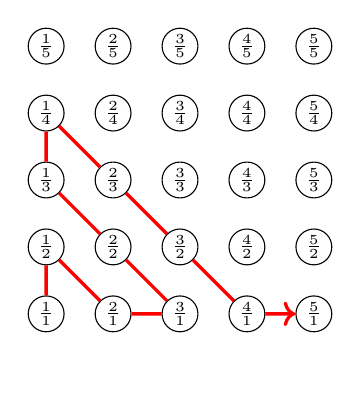
\begin{tikzpicture}[scale=.85,baseline={(0,0)}]
  \foreach \x in {1,...,5}{
    \foreach \y in {1,...,5}{
      \node[circle,inner sep=1pt,draw] (p-\x-\y) at (\x,\y) {\scriptsize $\frac{\x}{\y}$};
    }
  }
  % Zig-zag path (first few steps)
  \draw[very thick,red,->] (p-1-1)--(p-1-2)--(p-2-1)--(p-3-1)--(p-2-2)--(p-1-3)--(p-1-4)--(p-2-3)--(p-3-2)--(p-4-1)--(p-5-1);
  \end{tikzpicture}
  \]
  Skipping repetitions (keep only reduced fractions) we obtain an enumeration of $\mathbb{Q}_{+}$, i.e., an bijection from $\mathbb{Q}_{+}$ to $\N$. Therefore, $|\mathbb{Q}_{+}|=\aleph_0$.
\end{example}


Now let's see some criteria for countability.

\begin{lemma}
  Let $C\subset\N$ be infinite. Then $C$ is countably infinite.
\end{lemma}
\begin{proof}
  Define $f:\N\to C$ inductively as follows: let $f(1)=\min C$. If $f(1),\ldots,f(n)$ have been defined, let $f(n+1)=\min(C\setminus\{f(1),\ldots,f(n)\})$. 

  $f$ is injective: for $m<n$, $f(n)\in C\setminus\{f(1),\ldots,f(n-1)\}$, but $f(m)$ is not in the set. So, $f(n)\neq f(m)$.

  $f$ is surjective: for any $c\in C$, there exists $n\in\N$ such that $f(n)\geq c$. Let $m$ be the smallest integer with $f(m)\geq c$. So for any $i<m$, $f(i)<c$. So $c\notin\{f(1),\ldots,f(m-1)\}$ and hence $f(m)\leq c$ by its definition. This implies that $f(m)=c$.
\end{proof}

The same proof can be used to prove the following result.

\begin{proposition}
If $A$ is infinite, then $|A|\ge \aleph_0$.
\end{proposition}
\begin{proof}
  Since $A$ is infinite, so $A$ is not empty and hence we can choose $\leq$ to make $A$ well-ordered. We define a map $f:\N\to A$ inductive as follows: $f(1)=\min A$. If $f(1),\ldots,f(n)$ have been defined, let $f(n+1)=\min(A\setminus\{f(1),\ldots,f(n)\})$. Then, $f$ is injective. So $|A|\geq \aleph_0$.
\end{proof}

\begin{theorem}
  For any nonempty $A$, the following are equivalent:
  \begin{enumerate}
    \item $A$ is countable;
    \item there exists a surjection $f:\N\to A$;
    \item there exists an injection $g:A\to\N$.
  \end{enumerate}
\end{theorem}
\begin{proof}
  We prove the implications as follows:
  \begin{itemize}
    \item[$(1)\Rightarrow(2)$] If $A$ is countably finite, then there exists a bijection and hence surjection $f:\N\to A$. If $A$ is finite, then the composition is what we need: $\N\to \{1,\ldots,n\}\to A$.
    \item[$(2)\Rightarrow(3)$] If there exists a surjection $f:\N\to A$, then we can define an injection $g:A\to\N$ by $g(a)=\min\{n\in\N:f(n)=a\}$ for all $a\in A$.
    \item[$(3)\Rightarrow(1)$] If there exists an injection $g:A\to\N$, then we can decompose this as $A\to im(g)\to \N$. If $im(g)$ is finite, then $A$ is finite. If $im(g)$ is infinite, then by the lemma above, $im(g)$ is countably infinite and hence so is $A$.
  \end{itemize}
\end{proof}


% \begin{proposition}
% If $A$ is infinite, then $|A|\ge \aleph_0$.
% \end{proposition}
% \begin{proof}
%   Since $A$ is infinite, so $A$ is not empty. We can choose $a_1\in A$. Suppose we have chosen distinct elements $a_1,\ldots,a_n\in A$. Since $A$ is infinite, we can choose another element $a_{n+1}\in A\setminus\{a_1,\ldots,a_n\}$.  Continuing this process, we obtain a sequence of distinct elements \(a_1,a_2,\ldots\) in \(A\).  The map \(f\colon \mathbb{N}\to A\) defined by \(f(n)=a_n\) is an injection, hence \(|A|\geq |\N|=\aleph_0\).
% \end{proof}

% Can we obtain a set \(B\) such that \(|B|>\aleph_0\)?



\begin{theorem}
  The product of finitely many countable sets is countable. 
\end{theorem}

Instead of proving the general theorem, we show a special case.
\begin{proposition}
$|\N\times \N|=\aleph_0$.
\end{proposition}
\begin{proof}
  We can define a function \(f:\N\times\N\to\N\) by
  \[
  f(m,n) = 2^m 3^n.
  \]
  This function is injective, hence $\N\times\N$ is countable. Since $\N\times \N$ is obviously infinite, we have that $|\N\times\N|=\aleph_0$. 
\end{proof}

\fi

% The Fall 2026 Week 2 handout ends with Proposition 1.67.
\ifdefined\stopaftercountableproduct
  \expandafter\endinput
\fi

As a consequence, we have that taking countable unions still cannot increase cardinality.

\begin{theorem}
  Let $A_n$ be a countable set for each \(n\in\N\). Then $\bigcup_nA_n$ is countable.
\end{theorem}
\begin{proof}
  Since $A_n$ is countable, there is a surjection $f_n:\N\to A_n$. Define a function \(f:\N\times \N\to \bigcup_n A_n\) by
  \[
  f(m,n) = f_n(m).
  \]
  This function is surjective, hence \(\bigcup_n A_n\) is countable.
\end{proof}

How about the product of countably many countable sets?

\begin{theorem}
  $\{0,1\}^{\N}$ is uncountable. So the countable product of countable sets need not be countable.
\end{theorem}
\begin{proof}
  Suppose $\{0,1\}^{\N}$ were countable. Then we could list all infinite $0$–$1$ sequences as
  \[
  s^{(1)},s^{(2)},s^{(3)},\ldots,\qquad
  s^{(k)}=(s^{(k)}_1,s^{(k)}_2,s^{(k)}_3,\ldots),\ s^{(k)}_n\in\{0,1\}.
  \]
  Define a new sequence $t=(t_1,t_2,\ldots)$ by flipping the diagonal bits:
  \[
  t_n = 1 - s^{(n)}_n\quad (n\ge 1).
  \]
  Then $t\in\{0,1\}^{\N}$, but $t\neq s^{(k)}$ for every $k$ because they differ in the $k$‑th coordinate. This contradicts the assumption that the list was complete. Hence $\{0,1\}^{\N}$ is uncountable. 
\end{proof}

\newpage

\begin{corollary}
  $|\mathcal{P}(\N)|=|\{0,1\}^{\N}|>|\N|$.
\end{corollary}
\begin{proof}
  Define $\Phi:\{0,1\}^{\N}\to \mathcal{P}(\N)$ by
  \[
  \Phi\bigl((x_n)_{n\ge1}\bigr)=\{\,n\in\N: x_n=1\,\}.
  \]
  If $(x_n)\neq(y_n)$ pick $k$ with $x_k\neq y_k$; then $k$ belongs to exactly one of the two images, so $\Phi(x_n)\neq\Phi(y_n)$. Thus $\Phi$ is injective. Conversely, for any $A\subseteq\N$ let its characteristic sequence $\chi_A$ be given by $\chi_A(n)=1$ if $n\in A$, $0$ otherwise. Then $\Phi(\chi_A)=A$, so $\Phi$ is surjective. Hence $|\mathcal{P}(\N)|=|\{0,1\}^{\N}|$.
\end{proof}

In fact, this corollary is a special case of a more general result which we will prove later.

\begin{theorem}[Cantor's Theorem]
For any set $S$, there is no surjective function from $S$ to its power set $\mathcal{P}(S)$. In particular, $|S| < |\mathcal{P}(S)|$.
\end{theorem}

\begin{corollary}
  $|[0,1)|=|\{0,1\}^{\N}|>\aleph_0$.
\end{corollary}
\begin{proof}
  Define $E\subset \{0,1\}^{\N}$ to be the set of sequences that are not eventually all $1$. Define $\Phi:E\to[0,1)$ by
  \[
  \Phi\bigl((x_n)_{n\ge1}\bigr)=\sum_{n=1}^\infty \frac{x_n}{2^{\,n}}.
  \]
  This is surjective because for any $y\in[0,1)$, we can write $y$ in binary expansion $y=0.y_1y_2y_3\ldots$ with $y_i\in\{0,1\}$ and not ending with an infinite sequence of $1$'s (i.e., when $0.x_1\cdots x_{m-1}1\,0\,0\,0\cdots = 0.x_1\cdots x_{m-1}0\,1\,1\,1\cdots$ happens we choose the expansion that does not end with $1$'s). 
  
  This is also injective: 
  Let $(x_k),(y_k)\in E$ with $(x_k)\ne(y_k)$ and let $n$ be the first index where they differ. WLOG $x_n=0$ and $y_n=1$. Then
  \[
  \Phi(y)-\Phi(x)=\sum_{k=1}^{\infty}\frac{y_k-x_k}{2^k}
  =\frac{1}{2^n}+\sum_{k>n}\frac{y_k-x_k}{2^k}.
  \]
  Since $y_k-x_k\in\{-1,0,1\}$,
  \[
  \sum_{k>n}\frac{y_k-x_k}{2^k}\ge -\sum_{k>n}\frac{1}{2^k}=-\frac{1}{2^n},
  \]
  with equality only if $y_k-x_k=-1$ for all $k>n$, i.e. $x_k=1$ and $y_k=0$ for every $k>n$, which would make $(x_k)$ eventually $1$, contrary to $(x_k)\in E$. Hence the tail sum is strictly greater than $-1/2^n$, so $\Phi(y)-\Phi(x)>0$ and therefore $\Phi(x)\ne\Phi(y)$. 

Therefore, $|[0,1)|=|E|$. Now, we let $D\subset \{0,1\}^{\N}$ be the set of sequences that are eventually $1$. $E=\{0,1\}\setminus D$. We use the following two claims to finish the proof.
  
  \paragraph{Claim 1} $D$ is countable.

  \paragraph{Claim 2} An uncountable set minus a countable set will maintain its cardinality.

  Hence, we have $|E|=|\{0,1\}^{\N}|$. Hence $|[0,1)|=|\{0,1\}^{\N}|>\aleph_0$.

  We will leave Claim 1 as an exercise in your homework 2. We prove Claim 2 below.
\end{proof}


% \begin{proof}
%   For any element $x\in[0,1)$, write by decimals $x=0.a_1a_2a_3\ldots$ with $a_i\in\{0,1,2,\cdots,9\}$. We also make the assumption that the decimal representation does not end with an infinite sequence of 9's, so that $0.999\ldots=1$. So each element has a unique decimal representation.

%   Assume that $[0,1)$ is countable. Then, we can list its elements as $x_1,x_2,\ldots$. Assume that each $x_n$ has the decimal representation $x_n=0.a_{n,1}a_{n,2}a_{n,3}\ldots$. Consider the real number
%   \[
%   y = 0.b_1b_2b_3\ldots
%   \]
%   where $b_n = 3$ if $a_{n,n} \neq 3$, and $b_n = 4$ if $a_{n,n} = 3$. Then $y\in[0,1)$ and $y\neq x_n$ for all $n$, a contradiction.
% \end{proof}


\begin{proposition}
  Let $A$ be an infinite set and $F$ a finite set. Then,
  \begin{itemize}
    \item $|A\cup F|=|A|$.
    \item $|A\setminus F|=|A|$.
  \end{itemize}
  The conclusion still holds if $A$ is uncountable and $F$ is infinitely countable.
\end{proposition}
\begin{proof}
  Let $G:=F\setminus A$. Then $G$ is finite and disjoint from $A$. We need to show that $|A\cup G|=|A|$. Since $A$ is infinite, we can choose a sequence of distinct elements \(a_1,a_2,\ldots\) in \(A\).  If $G=\emptyset$, the result is trivial. If $G\neq\emptyset$, we write $G=\{g_1,g_2,\ldots,g_n\}$, where $n$ is finite. Define $f:A\to A\cup G$ as follows:
  \begin{enumerate}
    \item if $a\notin\{a_1,\ldots\}$, then set $f(a):=a$;
    \item if $a=a_i$ for some $i\leq n$, then set $f(a):=g_i$.
    \item If $a=a_i$ for some $i>n$, then set $f(a):=a_{i-n}$.
  \end{enumerate}
  Then, $f$ is a bijection. Thus $|A\cup G|=|A|$.

  For the second part, we let $B:=A\setminus F$. Then, $|A\setminus F|=|B|=|B\cup (A\cap F)|=|A|$.

  Now, assume that $F$ is countably infinite and $A$ is uncountable. Let $G:=F\setminus A$. Then, $G$ is countable. WLOG, we assume $G$ is infinite. We then can write $G=\{g_1,g_2,\ldots\}$. Still choose a sequence of distinct elements \(a_1,a_2,\ldots\) in \(A\). Define $f:A\to A\cup G$ as follows:
  \begin{enumerate}
    \item if $a\notin\{a_1,\ldots\}$, then set $f(a):=a$;
    \item if $a=a_{2n}$, then set $f(a_{2n}):=g_n$;
    \item if $a=a_{2n-1}$, then set $f(a_{2n-1}):=a_{n}$.
  \end{enumerate}
  Then, $f$ is a bijection. Thus $|A\cup G|=|A|$.

\end{proof}

\begin{corollary}
  $|[0,1)|=|[0,1]|=|(0,1)|=|(0,1]|$.
\end{corollary}

\begin{proposition}
  $|(0,1)|=|\mathbb{R}|$.
\end{proposition}
\begin{proof}
  Let $f:(0,1)\to\mathbb{R}$ be defined by
  \[
  f(x) = \tan\bigl((x-\tfrac{1}{2})\pi\bigr).
  \]
  Then $f$ is a bijection, hence $|(0,1)|=|\mathbb{R}|$.
\end{proof}

\begin{corollary}
  $|\R\setminus\Q|=|\R|$.
\end{corollary}






\subsubsection{Proofs of some general theorems}

\begin{theorem}[Cantor-Schröder-Bernstein]
If there exist injections \(f: A \to B\) and \(g: B \to A\), then there exists a bijection \(h: A \to B\).
\end{theorem}
\begin{proof}
WLOG, we assume that $A$ and $B$ are disjoint (otherwise replace $B$ by a disjoint copy). For each $a\in A$, we have the following sequence:
\[\ldots\overset{f}{\mapsto} b_{-3}\overset{g}{\mapsto} a_{-2}\overset{f}{\mapsto} b_{-1}\overset{g}{\mapsto} a_0=a\overset{f}{\mapsto} b_0\overset{g}{\mapsto} a_1\overset{f}{\mapsto} b_1\overset{g}{\mapsto} a_2\overset{f}{\mapsto} \ldots\]
There are only four possibilities for this sequence:
\begin{enumerate}
  \item ($B$-stopper) it stops at some $b_{-k}$ where $k\geq 1$. 
  \item ($A$-stopper) it stops at some $a_{-k}$ where $k\geq 0$.
  \item (bi-infinite) it continues indefinitely in both directions.
  \item (cyclic) it is a cyclic sequence, i.e., $a_i=a_j$ for some $i<j$.
\end{enumerate}

This also holds for any $b\in B$ and hence these four possibilities give rise to a partition of $A\sqcup B$.

Now, we define $h:A\to B$ as follows:
\[
h(a) =
\begin{cases}
f(a), & \text{if $a$ is an $A$-stopper};\\
f(a), & \text{if $a$ is in a bi-infinite chain or a cycle};\\
g^{-1}(a), & \text{if $a$ is a $B$-stopper}.
\end{cases}
\]

This is a bijection.
\end{proof}


We proved this using Well-ordering theorem. We can also prove this using Zorn's lemma.
\begin{theorem}
If $A,B$ are sets then either $|A|\le |B|$ or $|B|\le |A|$.
\end{theorem}

\begin{proof}
Let $\mathcal{M}$ be the set of \emph{matchings} between $A$ and $B$:
\[
\mathcal{M} = \{ M \subseteq A \times B \mid \text{each } a \in A \text{ appears in at most one pair of } M, \ \text{and each } b \in B \text{ appears in at most one} \}.
\]
We partially order $\mathcal{M}$ by inclusion.  
If $\{ M_i \}_{i \in I}$ is a chain in $\mathcal{M}$, then
\[
M = \bigcup_{i \in I} M_i
\]
is again a matching, since no element of $A$ or $B$ can be matched to more than one partner within a chain. Thus every chain has an upper bound.

By \emph{Zorn's Lemma}, $\mathcal{M}$ has a maximal element $M^\ast$.

Suppose there exist $a \in A$ and $b \in B$ both unmatched in $M^\ast$. Then
\[
M' = M^\ast \cup \{ (a,b) \}
\]
is a matching strictly larger than $M^\ast$, contradicting maximality. Therefore, at least one side is fully matched: either every $a \in A$ is matched, or every $b \in B$ is matched.

\begin{itemize}
    \item If every $a \in A$ is matched, define $f: A \to B$ by $f(a) = b$ whenever $(a,b) \in M^\ast$. This $f$ is injective, so $|A| \le |B|$.
    \item Otherwise, every $b \in B$ is matched. Define $g: B \to A$ by $g(b) = a$ whenever $(a,b) \in M^\ast$. Then $g$ is injective, so $|B| \le |A|$.
\end{itemize}

Thus, for any sets $A$ and $B$, either $|A| \le |B|$ or $|B| \le |A|$.
\end{proof}

\begin{theorem}[Cantor's Theorem]
For any set $S$, there is no surjective function from $S$ to its power set $\mathcal{P}(S)$. In particular, $|S| < |\mathcal{P}(S)|$.
\end{theorem}

\begin{proof}
Suppose $f\colon S\to \mathcal{P}(S)$ is any function. Define $B = \{s \in S : s \notin f(s)\}$. If $B\subseteq S$ is in the range of $f$, then there exists $s_0 \in S$ such that $f(s_0) = B$. The following contradictions arise: one can show that
\[s_0\in B \implies s_0\notin f(s_0) = B \quad\text{and}\quad s_0\notin B = f(s_0) \implies s_0\in B,\]
which forces a contradiction. Consequently any function $f\colon S\to \mathcal{P}(S)$ must fail to be surjective, and hence $|S|\neq |\mathcal{P}(S)|$. On the other hand, there is an obvious injection $S\to \mathcal{P}(S)$ given by $s\mapsto\{s\}$. Therefore
\[|S| < |\mathcal{P}(S)|<|\mathcal{P}(\mathcal{P}(S))|<\dots.
\]
\end{proof}

%---------------------------------------------------------------------------

\newpage


\section{Metric spaces}

% Offering-specific handouts may begin immediately after Example 2.2.
% Preserve the theorem numbering from the master notes.
\ifdefined\startafterexampletwotwo
  \setcounter{theorem}{2}
\else

For real functions $f:\R\to\R$, we have the notion of continuity using $\varepsilon$-$\delta$ definition: a function $f:\R\to\R$ is continuous at a point $x_0\in\R$ if for every $\varepsilon>0$ there exists $\delta>0$ such that
\[
|f(x)-f(x_0)|<\varepsilon \quad \text{whenever } |x-x_0|<\delta.
\]
We also have the notion of continuity using sequences: a function $f:\R\to\R$ is continuous at a point $x_0\in\R$ if for every sequence $(x_n)$ in $\R$ converging to $x_0$, the sequence $(f(x_n))$ converges to $f(x_0)$. 

In an attempt to generalize these notions to more general settings than $\R$, Frechet introduced the notion of metric spaces in 1906. Metric spaces provide a natural setting to generalize the notions of continuity above. Later, Hausdorff introduced the more general notion of topological spaces in 1914. We will first study metric spaces and then topological spaces.

\begin{definition}[Metric Space]
A \emph{metric space} is a pair $(X,d)$ consisting of a set $X$ and a
function $d\colon X\times X\to [0,\infty)$ called a \emph{metric} such that
\begin{enumerate}
  \item $d(x,y)=0$ if and only if $x=y$;
  \item $d(x,y)=d(y,x)$ for all $x,y\in X$ (symmetry);
  \item $d(x,z)\le d(x,y)+d(y,z)$ for all $x,y,z\in X$ (triangle inequality).
\end{enumerate}
The value $d(x,y)$ is called the \emph{distance} between points $x$ and $y$ in the metric space.

If $(X,d)$ satisfies 2 and 3 and 1' below, it is called a \emph{pseudometric space}. 

1'. $d(x,x)=0$ for all $x\in X$.
\end{definition}

\begin{example}
  \begin{enumerate}
    \item $X=\R^n$, $d_p(x,y)=\|x-y\|_p=\left(\sum_{i=1}^n |x_i-y_i|^p\right)^{1/p}$ for $1\le p<\infty$ and $d_\infty(x,y)=\|x-y\|_\infty=\max_{1\le i\le n}|x_i-y_i|$ are metrics on $\R^n$. 
    \item Let $X$ be any set and $f:X\to \R$ be any function. Then, the following defines a pseudometric on $X$:
      \[
      d(x,y) = |f(x)-f(y)|.
      \]
    \item Let $(X,d)$ be a metric space and $A\subset X$ be a nonempty subset. Then, $(A,d|_{A\times A})$ is a metric space, called a \emph{subspace} of $(X,d)$.
  \end{enumerate}
\end{example}

\fi

% Offering-specific weekly handouts may stop after Example 2.2.
\ifdefined\stopafterexampletwotwo
  \expandafter\endinput
\fi



\begin{definition}
  Let $(X,d_X)$ and $(Y,d_Y)$ be metric spaces. A function $f\colon X\to Y$ is called an isometric embedding if
  \[
  d_Y(f(x),f(x'))=d_X(x,x') \quad \text{for all } x,x'\in X.
  \]
  The function $f$ is called an isometry if it is an isometric embedding that is also surjective and we say that $(X,d_X)$ and $(Y,d_Y)$ are \emph{isometric} if there exists an isometry between them.
\end{definition}

\begin{example}[Isometric embedding]
Let $f:\R\to\R^2$ be given by $f(t)=(t,0)$. For $s,t\in\R$,
\[
\|f(s)-f(t)\|_2=\sqrt{(s-t)^2+0^2}=|s-t|.
\]
Thus $f$ preserves distances (an isometric embedding). It is not surjective, so it is not an isometry. Its image is the $x$-axis in $\R^2$.

Is the map $g(x):=(x,x)$ an isometric embedding?
\end{example}





\begin{definition}
  Let $(X,d_X)$ and $(Y,d_Y)$ be metric spaces. A function $f\colon X\to Y$ is called \emph{Lipschitz continuous} if there exists a constant $L\ge 0$ such that
  \[
  d_Y(f(x),f(x'))\le L \cdot d_X(x,x') \quad \text{for all } x,x'\in X.
  \]
\end{definition}

\begin{definition}
  Let $(X,d_X)$ and $(Y,d_Y)$ be metric spaces. A function $f\colon X\to Y$ is called \emph{continuous} at a point $x_0\in X$ if for every $\varepsilon>0$ there exists $\delta>0$ such that
  \[
  d_Y(f(x),f(x_0))<\varepsilon \quad \text{whenever } d_X(x,x_0)<\delta.
  \]
  The function $f$ is called \emph{continuous} if it is continuous at every point $x_0\in X$.
\end{definition}


\begin{proposition}
  Any Lipschitz continuous function between metric spaces is continuous. Any isometric embedding is also Lipschitz continuous.
\end{proposition}
\begin{proof}
  Let $f:X\to Y$ be Lipschitz continuous with constant $L$. Given $\varepsilon>0$, let $\delta=\varepsilon/L$. Then, for any $x\in X$ with $d_X(x,x_0)<\delta$, we have
  \[
  d_Y(f(x),f(x_0))\le L\cdot d_X(x,x_0)<L\cdot \frac{\varepsilon}{L}=\varepsilon.
  \]
  Thus, $f$ is continuous at $x_0$. Since $x_0$ is arbitrary, $f$ is continuous.

  If $f$ is an isometric embedding, then for any $x,x'\in X$, we have
  \[
  d_Y(f(x),f(x'))=d_X(x,x')\le 1\cdot d_X(x,x').
  \]
  Thus, $f$ is Lipschitz continuous with constant $L=1$.
\end{proof}



\subsection{Characterizations of continuity}

\subsubsection{A sequential characterization of continuity}

For real functions, we can define continuity using sequences. This can be generalized to metric spaces as well.

\begin{definition}
    A sequence $(x_n)_{n\in\mathbb{N}}$ in a metric space $(X,d)$ is said to converge to a point $x\in X$ if for every $\epsilon>0$, there exists $N\in\mathbb{N}$ such that $d(x_n,x)<\epsilon$ for all $n\ge N$.
\end{definition}

One can characterize continuity using sequences:
\begin{proposition}
    A function $f:X\to Y$ is continuous at a point $x_0\in X$ if and only if for every sequence $(x_n)_{n\in\mathbb{N}}$ in $X$ converging to $x_0$, the sequence $(f(x_n))_{n\in\mathbb{N}}$ converges to $f(x_0)$.
\end{proposition}
\begin{proof}
  Suppose first that $f$ is continuous at $x_0$, and let $(x_n)_{n\in\mathbb{N}}$ be a sequence converging to $x_0$. For any $\varepsilon>0$, by continuity there exists $\delta>0$ such that
  \[
  d_X(x,x_0)<\delta \quad\Longrightarrow\quad d_Y(f(x),f(x_0))<\varepsilon.
  \]
  Since $(x_n)$ converges to $x_0$, there exists an $N\in\mathbb{N}$ with $d_X(x_n,x_0)<\delta$ for all $n\ge N$. Hence, for all $n\ge N$, we have
  \[
  d_Y(f(x_n),f(x_0))<\varepsilon,
  \]
  so $(f(x_n))$ converges to $f(x_0)$.

  Conversely, suppose that for every sequence $(x_n)$ converging to $x_0$, the sequence $(f(x_n))$ converges to $f(x_0)$. Assume for contradiction that $f$ is not continuous at $x_0$. Then there exists $\varepsilon_0>0$ such that for every $\delta>0$ there exists some $x\in X$ with
  \[
  d_X(x,x_0)<\delta \qquad\text{but}\qquad d_Y(f(x),f(x_0))\ge \varepsilon_0.
  \]
  For each $n\in\mathbb{N}$, choosing $\delta=\frac{1}{n}$, there exists $x_n\in X$ with
  \[
  d_X(x_n,x_0)<\frac{1}{n} \quad\text{and}\quad d_Y(f(x_n),f(x_0))\ge \varepsilon_0.
  \]
  Then $(x_n)$ converges to $x_0$, yet $(f(x_n))$ cannot converge to $f(x_0)$ since the distance remains at least $\varepsilon_0$, which is a contradiction.
\end{proof}

\subsubsection{A open set characterization of continuity}

\begin{definition}
  Let $(X,d)$ be a metric space. For any $x\in X$ and $r>0$, the \emph{open ball} of radius $r$ centered at $x$ is defined as
  \[
  B_r(x) = \{y\in X:d(x,y)<r\}.
  \]
\end{definition}

\begin{example}[Shapes of balls for different metrics on \(\R^2\)]
For \(r>0\) the open unit balls (centered at the origin) for the standard metrics on \(\R^2\) have the following shapes:
\[
\begin{aligned}
B_r^{(2)}(0) &= \{x\in\R^2 : \|x\|_2 < r\}      &&\text{(Euclidean) — disk},\\
B_r^{(1)}(0) &= \{x\in\R^2 : |x_1|+|x_2| < r\}  &&\text{(Taxicab / \(\ell^1\)) — diamond},\\
B_r^{(\infty)}(0) &= \{x\in\R^2 : \max(|x_1|,|x_2|) < r\} &&\text{(Maximum / \(\ell^\infty\)) — square}.
\end{aligned}
\]
Below we draw the case \(r=1\).
\end{example}

\begin{figure}[h]
  \centering
  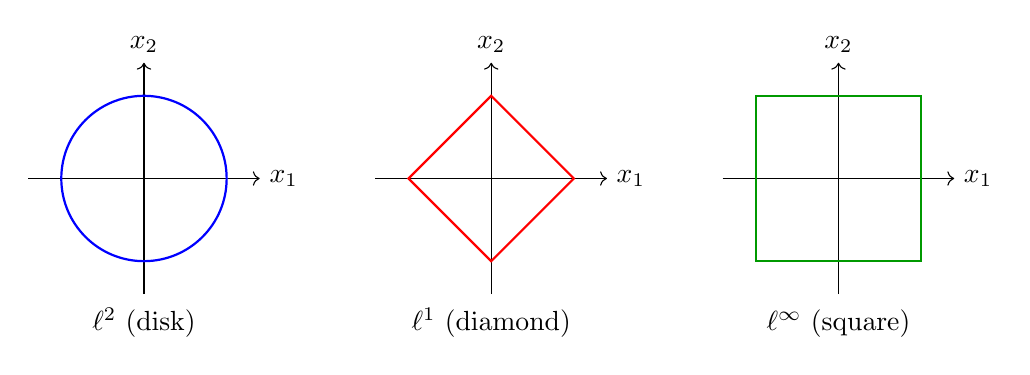
\begin{tikzpicture}[scale=1.05]
    % Euclidean ball
    \begin{scope}
      \draw[->] (-1.4,0)--(1.4,0) node[right]{$x_1$};
      \draw[->] (0,-1.4)--(0,1.4) node[above]{$x_2$};
      \draw[thick,blue] (0,0) circle (1);
      \node at (0,-1.75) {\(\ell^2\) (disk)};
    \end{scope}
    % Taxicab ball
    \begin{scope}[xshift=4.2cm]
      \draw[->] (-1.4,0)--(1.4,0) node[right]{$x_1$};
      \draw[->] (0,-1.4)--(0,1.4) node[above]{$x_2$};
      \draw[thick,red] (0,1)--(1,0)--(0,-1)--(-1,0)--cycle;
      \node at (0,-1.75) {\(\ell^1\) (diamond)};
    \end{scope}
    % Infinity ball
    \begin{scope}[xshift=8.4cm]
      \draw[->] (-1.4,0)--(1.4,0) node[right]{$x_1$};
      \draw[->] (0,-1.4)--(0,1.4) node[above]{$x_2$};
      \draw[thick,green!60!black] (-1,-1) rectangle (1,1);
      \node at (0,-1.75) {\(\ell^\infty\) (square)};
    \end{scope}
  \end{tikzpicture}
  \caption{Unit balls \(B_1(0)\) in \(\R^2\) for \(\ell^2,\ \ell^1,\ \ell^\infty\) metrics.}
\end{figure}

Then, we can rewrite the definition of continuity using open balls.

\begin{proposition}
  A function $f:X\to Y$ between metric spaces $(X,d_X)$ and $(Y,d_Y)$ is continuous at a point $x_0\in X$ if and only if for every $r>0$, there exists $\delta>0$ such that
  \[
  f(B_\delta(x_0))\subseteq B_r(f(x_0)).
  \]
\end{proposition}

The definition of open balls of course depends on the metric. Suppose you want to generalize everything so far to the setting when you don't have metric. Then, let's try to define some language where the notion of metric will be hidden. 

\begin{definition}
      A subset $U\subseteq X$ is called \emph{open} if for every point $x\in U$ there exists a radius $r>0$ such that the open ball $B_r(x)$ is contained in $U$.
\end{definition}

\begin{proposition}
  Any open ball $B_r(x)$ is open.
\end{proposition}
\begin{proof}
  Let's prove the last item. Let $x\in B_r(x_0)$ for some $r>0$. Pick $r':=r-d_X(x,x_0)$. Then, $B_{r'}(x)\subseteq B_r(x_0)$.
\end{proof}

\begin{corollary}
  Let $(X,d)$ be a metric space and $U\subseteq X$ be a subset. Then, $U$ is open iff $U$ is a union of open balls.
\end{corollary}

\begin{proof}
  Assume that $U$ is open. Then, for every $x\in U$ there exists $r_x>0$ so that $B_{r_x}(x)\subseteq U$. Thus, we can write
  \[
  U = \bigcup_{x\in U} B_{r_x}(x).
  \]

  Conversely, if $U=\bigcup_{i\in I}B_{r_i}(x_i)$ is a union of open balls, then for every $x\in U$, we have that $x\in B_{r_i}(x_i)$ for some $i\in I$. This means that there exists a radius $r>0$ such that $B_r(x)\subseteq B_{r_i}(x_i)\subseteq U$. Thus, $U$ is open.
\end{proof}

% \begin{proposition}
%   Let $(X,d)$ be a metric space.
%   \begin{enumerate}
%     \item The empty set is open
%     \item The whole space $X$ is open.
%     \item Any union of open sets is open.
%     \item The intersection of two open sets is open. Hence, the intersection of any finite number of open sets is open.
%   \end{enumerate}
% \end{proposition}

Now we can revisit the definition of continuous functions.

\begin{theorem}
  Let $f:X\to Y$ be a function between metric spaces $(X,d_X)$ and $(Y,d_Y)$. Then $f$ is continuous at a point $x_0\in X$ if and only if for every open set $V\subseteq Y$ containing $f(x_0)$, there exists an open set $U\subseteq X$ containing $x_0$ such that $f(U)\subseteq V$. 
\end{theorem}
\begin{proof}
  Suppose that $f$ is continuous at $x_0$. Let $V\subseteq Y$ be an open set containing $f(x_0)$. By openness, there exists $r>0$ such that $B_r(f(x_0))\subseteq V$. By continuity, there exists $\delta>0$ such that $f(B_\delta(x_0))\subseteq B_r(f(x_0))\subseteq V$. Thus, we can take $U=B_\delta(x_0)$.

  Conversely, suppose that for every open set $V\subseteq Y$ containing $f(x_0)$, there exists an open set $U\subseteq X$ containing $x_0$ such that $f(U)\subseteq V$. Given $\varepsilon>0$, let $V=B_\varepsilon(f(x_0))$. By assumption, there exists an open set $U\subseteq X$ containing $x_0$ such that $f(U)\subseteq V$. Since $U$ is open and contains $x_0$, there exists $\delta>0$ such that $B_\delta(x_0)\subseteq U$. Thus,
  \[
  f(B_\delta(x_0))\subseteq f(U)\subseteq V = B_\varepsilon(f(x_0)).
  \]
  This shows that $f$ is continuous at $x_0$. 
\end{proof}

Finally, we will be able to establish the following characterization from the theorem above. We will not give a proof here as we will give a proof in a more general setting (topological spaces) later.

\begin{theorem}
  $f$ is continuous if and only if for every open set $V\subseteq Y$, the preimage $f^{-1}(V)$ is open in $X$.
\end{theorem}

The above theorem reads "preimage of open is open".


\subsubsection{A closed set characterization of continuity}
However, I never find this characterization natural to understand. We can think of the continuity as not ripping apart the space at any given point. More precisely, if a point is ``in touch'' with some region in the domain, it should remain in touch with the corresponding region in the codomain.

\begin{figure}[h!]
\centering
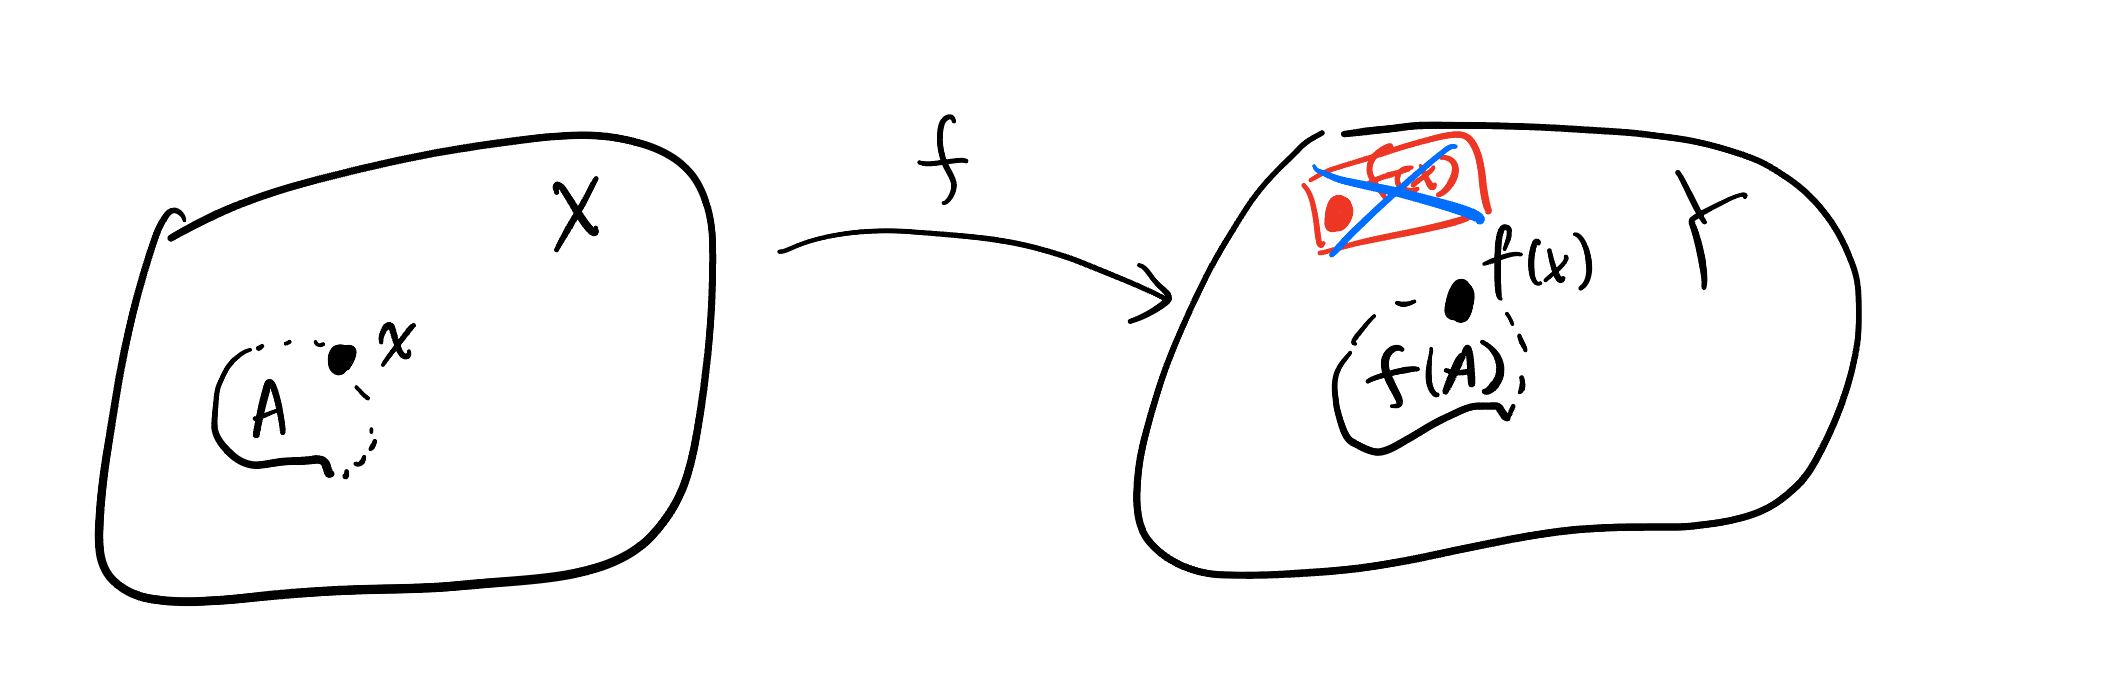
\includegraphics[width=0.8\textwidth]{figures/close-continuity.png}
\label{fig:close-continuity}
\end{figure}


\begin{definition}
  A subset $A\subseteq X$ is called \emph{closed} if its complement $X\setminus A$ is open. 
\end{definition}
% \begin{proposition}
%   Let $(X,d)$ be a metric space.
%   \begin{enumerate}
%     \item The empty set is closed.
%     \item The whole space $X$ is closed.
%     \item Any intersection of closed sets is closed.
%     \item The union of two closed sets is closed. Hence, the union of any finite number of closed sets is closed.
%   \end{enumerate}
% \end{proposition}


\begin{definition}
  For any set $A\subseteq X$, the \emph{closure} of $A$, denoted $\overline{A}$, is the smallest closed set containing $A$. Equivalently, it is the intersection of all closed sets containing $A$.
\end{definition}

\begin{theorem}\label{thm:image-closure}
  Let $f:X\to Y$ be a function between metric spaces $(X,d_X)$ and $(Y,d_Y)$. Then $f$ is continuous if and only if $f(\overline{A})\subseteq\overline{f(A)}$
\end{theorem}

The theorem above reads "image of closure is contained in closure of image", or more intuitively, "points that are in touch with a set remains in touch after the map".


Now we prove the theorem.

\begin{lemma}
  Let $A\subseteq X$ be a set. Then,
  \[\overline{A} = \{x\in X : \text{there exists a sequence }(x_n)_{n\in\mathbb{N}}\text{ in }A\text{ converging to }x\}.\]
\end{lemma}
\begin{proof}
  Let $x\in\overline{A}$. Consider any $r>0$. If $B_r(x)\cap A=\emptyset$, then the complement $X\backslash B_r(x)\supset A$. But this contradicts the fact that $x\in\overline{A}$. Now let $r_n:=1/n$. Then, pick $x_n\in B_{r_n}(x)\cap A$. Then, $(x_n)$ is a sequence in $A$ converging to $x$.

  Conversely, let $x\in X$ be such that there exists a sequence $(x_n)_{n\in\mathbb{N}}$ in $A$ converging to $x$. Consider a closed set $C\supset A$. If $x\notin C$, then there exists $r>0$ such that $B_r(x)\cap C=\emptyset$ (why?). This implies that $B_r(x)\cap A=\emptyset$ which contradicts the fact that $(x_n)$ converges to $x$. Thus, $x\in C$. Since $C\supset A$ is arbitrary, we have $x\in\overline{A}$. 
\end{proof}

Now, we prove \Cref{thm:image-closure}.
\begin{proof}[Proof of \Cref{thm:image-closure}]
  Suppose that $f$ is continuous. Let $x\in\overline{A}$. By the lemma, there exists a sequence $(x_n)$ in $A$ converging to $x$. By continuity, $(f(x_n))$ converges to $f(x)$. Since each $f(x_n)\in f(A)$, by the lemma again, we have $f(x)\in\overline{f(A)}$. Thus, $f(\overline{A})\subseteq\overline{f(A)}$.

  Conversely, suppose that $f(\overline{A})\subseteq\overline{f(A)}$ for every set $A\subseteq X$. Let $x_0\in X$ and let $(x_n)$ be a sequence converging to $x_0$. Assume on the contrary that $(f(x_n))$ does not converge to $f(x_0)$. Then, there exists $\varepsilon>0$ such that there is a subsequence $(f(x_{k_n}))$ such that $d_Y(f(x_{k_n}),f(x_0))\ge \varepsilon$ for all $n\in\mathbb{N}$.

  Now we let $A=\{x_{k_n}:n\in\mathbb{N}\}$. Then, $x_0\in\overline{A}$. Thus, $f(x_0)\in f(\overline{A})\subseteq \overline{f(A)}$. By the lemma, there exists a sequence $(y_n)$ in $f(A)$ converging to $f(x_0)$. But this is not possible due to the $\epsilon$ constraint. Therefore, we conclude that $(f(x_n))$ must converge to $f(x_0)$.
\end{proof}

We now see that many intuitive properties of continuous real functions can be generalized nicely to metric spaces. We will see that the open and closed language still works well in the more general setting of topological spaces, while the sequential language does not. In Willard's book, a whole chapter is devoted to the study of sequences in topological spaces.

\subsection{Ultrametric}
There is a special class of metric spaces called ultrametric spaces, which satisfy a stronger version of the triangle inequality. Ultrametric spaces have some interesting properties that are not shared by general metric spaces.

\begin{definition}[Ultrametric space]
A metric space $(X,d)$ is an \emph{ultrametric space} if $d$ satisfies the
\emph{strong triangle inequality}
\[
d(x,z)\le \max\{d(x,y),d(y,z)\}\qquad \text{for all }x,y,z\in X.
\]
We would usually use $u$ instead of $d$ to denote an ultrametric.
\end{definition}

\begin{proposition}
  Let $(X,u)$ be an ultrametric space. Then,
\begin{enumerate}
  \item If $r>0$ and $x,y\in X$ with $u(x,y)<r$, then $B_r(x)=B_r(y)$.
  \item Any two open balls are either disjoint or one contains the other.
  \item Every triangle is isosceles, i.e., if $x,y,z\in X$, then at least two of the distances $u(x,y)$, $u(y,z)$, and $u(z,x)$ are equal, and the third is less than or equal to the common value.
\end{enumerate}
\end{proposition}

\begin{example}
  Recall the definition of the Cantor set $C\subseteq [0,1]$: it is constructed by repeatedly removing the open middle third from each interval. More precisely, set $C_0 = [0,1]$, and for each $k\ge 1$, let $C_k$ be the union of $2^k$ closed intervals obtained by removing the open middle third from each interval in $C_{k-1}$. The Cantor set is defined as
  \[
  C = \bigcap_{k=0}^\infty C_k.
  \]
  Equivalently, $C$ consists of all numbers in $[0,1]$ whose base-3 expansion contains only the digits $0$ and $2$.
  We endow the Cantor set $C\subseteq [0,1]$ with the ultrametric as follows:
  \[
  d_C(x,y) =
  \begin{cases}
  0 & \text{if } x=y,\\[1ex]
  3^{-n} & \text{if } x\neq y \text{ and } n = \min\{ k \ge 0 : \text{$x$ and $y$ lie in different segments in } C_k \}.
  \end{cases}
  \]
\end{example}

It is perhaps difficult for you to understand what happens in the example above. It turns out that one can always create a nice visualization of ultrametric spaces using trees. We will use this to help us understand ultrametric spaces better. Although the following definition is for finite sets, it can be generalized to infinite sets as well.

\newpage

\begin{definition}
  \textbf{Dendrogram (finite case).}
  Let $X$ be finite. A dendrogram on $X$ is an order preserving map $\theta:[0,\infty)\to Part(X)$ on $X$ such that:
  \begin{enumerate}
    \item $\theta(0)$ is the discrete partition of $X$;
    \item there exists $T>0$ such that $\theta(T)$ is the trivial partition;
    \item for any $t\geq 0$, there exists $\epsilon>0$ such that $\theta(t)=\theta(t+\epsilon)$.
  \end{enumerate}
\end{definition}
\begin{example}
  Consider $X=\{a,b,c\}$. Define $\theta:[0,\infty)\to Part(X)$ by
  \[
  \theta(t) =
  \begin{cases}
    \{\{a\},\{b\},\{c\}\} & \text{if } 0\le t<1 \\
    \{\{a,b\},\{c\}\} & \text{if } 1\le t<2 \\
    \{\{a,b,c\}\} & \text{if } t\ge 2
  \end{cases}
  \]
  Notice that the strict inequalities cannot be replaced with non-strict inequalities, as this would violate the last condition.
\end{example}



\begin{theorem}[Finite dendrograms and ultrametrics are equivalent]
Let $X$ be a finite set. Let $\mathcal{D}(X)$ be the set of dendrograms on $X$ and $\mathcal{U}(X)$ be the set of ultrametrics on $X$. There are two maps between $\mathcal{D}(X)$ and $\mathcal{U}(X)$ as follows:
\begin{enumerate}
  \item (From dendrogram to ultrametric) Given a dendrogram $\theta$ on $X$, define
  \[
    u(x,y):=\inf\{t\ge 0:\ x, y \text{ belong to the same block in }\theta(t)\}\quad (x,y\in X).
  \]
  Then $u$ is an ultrametric on $X$.
  \item (From ultrametric to dendrogram) Given an ultrametric $u$ on $X$ set, we define an equivalence relation $\sim_t$ for $t\ge 0$,
  \[
    x\sim_t y \;\Longleftrightarrow\; u(x,y)\le t.
  \]
  Then we define $\theta$ by $\theta(t):=\{[x]_t:x\in X\}$ where $[x]_t$ is the equivalence class of $x$ under $\sim_t$. This gives a dendrogram on $X$.
\end{enumerate}
The above two maps, denoted by $\mathcal{D}: \mathcal{D}(X) \to \mathcal{U}(X)$ and $\mathcal{U}: \mathcal{U}(X) \to \mathcal{D}(X)$ respectively, are inverses of each other.
\end{theorem}

\begin{example}
  Consider the dendrogram $\theta$ on $X=\{a,b,c\}$ defined in the previous example. The corresponding ultrametric $u$ is given by
  \[
  u(x,y) =
  \begin{cases}
    0 & \text{if } x=y,\\
    1 & \text{if } \{x,y\}=\{a,b\},\\
    2 & \text{if } \{x,y\}=\{a,c\}\text{ or }\{b,c\}.
  \end{cases}
  \]
  Conversely, starting from this ultrametric $u$, we can recover the original dendrogram $\theta$.
\end{example}

% \begin{proof}[Proof sketch]
% (1) Symmetry and $u(x,x)=0$ are immediate. If $x\neq y$, discreteness at $t=0$ gives $u(x,y)>0$.
% For the strong triangle inequality: if $u(x,z)>s:=\max\{u(x,y),u(y,z)\}$ then
% $x\not\sim_s z$ while $x\sim_s y$ and $y\sim_s z$, contradicting transitivity of $\sim_s$.
% Hence $u(x,z)\le s$.

% (2) Each $\sim_t$ is an equivalence relation: reflexivity and symmetry are clear; for transitivity,
% if $u(x,y)\le t$ and $u(y,z)\le t$, the ultrametric inequality gives $u(x,z)\le t$.
% Monotonicity in $t$ is obvious; discreteness at $0$ and eventual totality follow since $X$ is finite
% and only finitely many pairwise distances occur. Piecewise constancy comes from the finite,
% ordered list of distinct positive distances.

% (3) Direct from the definitions: in the first direction $u(x,y)$ is exactly the merge level of $x,y$,
% and in the second $u(x,y)=\inf\{t:u(x,y)\le t\}=u(x,y)$.
% \end{proof}


% \subsection{Hausdorff distance}

% Let $(X,d_X)$ and $(Y,d_Y)$ be two metric spaces. The \emph{Hausdorff distance} between two non-empty subsets $A,B\subseteq X$ is defined as
% \[
% d_H(A,B) := \max\left\{ \sup_{a\in A} \inf_{b\in B} d_X(a,b), \sup_{b\in B} \inf_{a\in A} d_X(a,b) \right\}.
% \]
% Intuitively, the Hausdorff distance measures how far apart the sets $A$ and $B$ are from each other.

% TODO: insert further examples and properties of metric spaces as needed.

%---------------------------------------------------------------------------
% Section 3: Topological spaces (Willard §§2–9)
%---------------------------------------------------------------------------

\newpage


\section{Topological spaces and continuous functions}

This section introduces the notion of a topological space, which abstracts
the concept of ``openness'' captured by metric spaces.

\begin{definition}[Topological Space]
A \emph{topology} on a set $X$ is a family ${\tau}$ of subsets of $X$ (called \emph{open sets}) satisfying:
\begin{enumerate}
\item Both $\varnothing$ and $X$ belong to ${\tau}$;
\item Arbitrary unions of sets in ${\tau}$ belong to ${\tau}$: if $\{U_i\}_{i\in I}\subseteq{\tau}$, then $\bigcup_{i\in I} U_i\in{\tau}$;
\item Finite intersections of sets in ${\tau}$ belong to ${\tau}$: if $\{V_j\}_{j=1}^n\subseteq{\tau}$, then $\bigcap_{j=1}^n V_j\in{\tau}$.
\end{enumerate}
The pair $(X,{\tau})$ is called a \emph{topological space}. In many cases, we will omit the mention of the topology and simply refer to the space $X$.
\end{definition}

\begin{definition}
  Let $(X,{\tau})$ be a topological space. A subset $A\subseteq X$ is called \emph{closed} if its complement $X\setminus A$ is open, i.e., $X\setminus A\in{\tau}$.
\end{definition}
\begin{proposition}
  \begin{enumerate}
    \item $X$ and $\varnothing$ are closed.
    \item Any finite union of closed sets is closed.
    \item Any arbitrary intersection of closed sets is closed.
  \end{enumerate}
\end{proposition}
\begin{remark}
  A topology, i.e., the collection of open sets, can be equivalently described by the collection of closed sets.
\end{remark}

\begin{example}
Which of the following collections of subsets of \(X=\{a,b,c\}\) are topologies?
\begin{center}
\begin{tikzcd}[column sep=18mm,row sep=12mm]
% 1: indiscrete
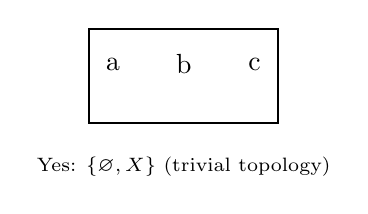
\begin{tikzpicture}[baseline=(base)]
  \node (base) at (0,0) {};
  \node at (0,0.15) {a};
  \node at (0.9,0.15) {b};
  \node at (1.8,0.15) {c};
  \draw[thick] (-0.3,-0.6) rectangle (2.1,0.6);
  \node[below=3pt] at (0.9,-0.8) {\scriptsize Yes: $\{\varnothing,X\}$ (trivial topology)};
\end{tikzpicture}
&
% 2: singletons a,b only (not a topology)
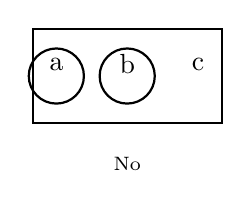
\begin{tikzpicture}[baseline=(base)]
  \node (base) at (0,0) {};
  \node at (0,0.15) {a};
  \node at (0.9,0.15) {b};
  \node at (1.8,0.15) {c};
  \draw[thick] (-0.3,-0.6) rectangle (2.1,0.6);
  \draw[thick] (0,0) circle (0.35); % {a}
  \draw[thick] (0.9,0) circle (0.35); % {b}
  \node[below=3pt] at (0.9,-0.8) {\scriptsize No};
\end{tikzpicture}
\\
% 3: two overlapping pairs (not closed under intersection -> missing {b})
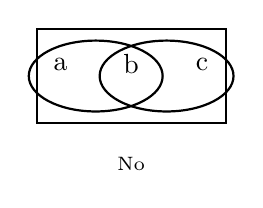
\begin{tikzpicture}[baseline=(base)]
  \node (base) at (0,0) {};
  \node at (0,0.15) {a};
  \node at (0.9,0.15) {b};
  \node at (1.8,0.15) {c};
  \draw[thick] (-0.3,-0.6) rectangle (2.1,0.6);
  \draw[thick] (0.45,0) ellipse (0.85 and 0.45); % {a,b}
  \draw[thick] (1.35,0) ellipse (0.85 and 0.45); % {b,c}
  \node[below=3pt] at (0.9,-0.8) {\scriptsize No};
\end{tikzpicture}
&
% 4: discrete with extra large circles around {a,b} and {b,c}
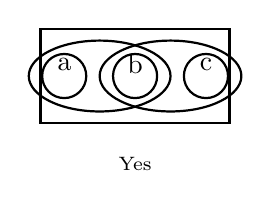
\begin{tikzpicture}[baseline=(base)]
  \node (base) at (0,0) {};
  \node at (0,0.15) {a};
  \node at (0.9,0.15) {b};
  \node at (1.8,0.15) {c};
  \draw[thick] (-0.3,-0.6) rectangle (2.1,0.6);
  % large ellipses circling {a,b} and {b,c}
  \draw[thick] (0.45,0) ellipse (0.9 and 0.45); % {a,b}
  \draw[thick] (1.35,0) ellipse (0.9 and 0.45); % {b,c}
  % individual points
  \draw[thick] (0,0) circle (0.28);
  \draw[thick] (0.9,0) circle (0.28);
  \draw[thick] (1.8,0) circle (0.28);
  \node[below=3pt] at (0.9,-0.8) {\scriptsize Yes};
\end{tikzpicture}
\\
% 5: topology with {b} and {a,b}
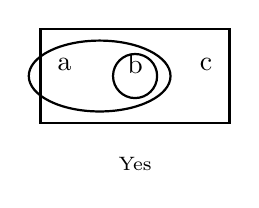
\begin{tikzpicture}[baseline=(base)]
  \node (base) at (0,0) {};
  \node at (0,0.15) {a};
  \node at (0.9,0.15) {b};
  \node at (1.8,0.15) {c};
  \draw[thick] (-0.3,-0.6) rectangle (2.1,0.6);
  \draw[thick] (0.45,0) ellipse (0.9 and 0.45); % {a,b}
  \draw[thick] (0.9,0) circle (0.28); % {b}
  \node[below=3pt] at (0.9,-0.8) {\scriptsize Yes};
\end{tikzpicture}
&
% 6: {a},{b},{a,b} present (topology)
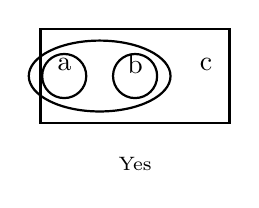
\begin{tikzpicture}[baseline=(base)]
  \node (base) at (0,0) {};
  \node at (0,0.15) {a};
  \node at (0.9,0.15) {b};
  \node at (1.8,0.15) {c};
  \draw[thick] (-0.3,-0.6) rectangle (2.1,0.6);
  \draw[thick] (0,0) circle (0.28); % {a}
  \draw[thick] (0.9,0) circle (0.28); % {b}
  \draw[thick] (0.45,0) ellipse (0.9 and 0.45); % {a,b}
  \node[below=3pt] at (0.9,-0.8) {\scriptsize Yes};
\end{tikzpicture}
\end{tikzcd}
\end{center}
\end{example}

\begin{example}
  Every metric space is a topological space with the open sets defined previously.
  
  As a special example, for $\R$, every open ball is a bounded open interval $(a,b)$. Hence, every open set in $\R$ is a union of disjoint open intervals (including unbounded intervals).

  Let $(X,\tau)$ be a topological space. If there exists a metric $d$ on $X$ such that open sets for $d$ coincide with $\tau$, we say $(X,\tau)$ is \emph{metrizable}.
\end{example}


\begin{example}
  Let $X$ be any set. Let ${\tau}:=P(X)$. Then, ${\tau}$ is a topology on $X$ and it is called the \emph{discrete topology}. This topology is induced by the discrete metric $d(x,y)=1$ if $x\neq y$ and $d(x,x)=0$.
\end{example}

\begin{example}
  Let $X$ be any set. Let ${\tau}:=\{\emptyset,X\}$. This is the \emph{trivial topology}. Is this metrizable?
\end{example}

\begin{lemma}
  For a metric space $(X,d)$, any point $x\in X$ forms a closed set, i.e., $\{x\}$ is closed.
\end{lemma}
\begin{proof}
  We show that $X\setminus\{x\}$ is open. For any $y\in X\setminus\{x\}$, let $r=d(x,y)/2>0$. Then, the open ball $B(y,r)\subseteq X\setminus\{x\}$. Hence, $X\setminus\{x\}$ is open.
\end{proof}

Now, for any set $X$ with more than two elements, the trivial topology is not metrizable since singletons are not closed.

\begin{example}
   Let $X$ be any set. Let ${\tau}:=\{O\subset X\mid O=\emptyset\ \text{or}\ X\setminus O \text{ is finite}\}$. Then ${\tau}$ is a topology on $X$ called the \emph{finite complement topology}.

    If $X=\R$, a nonempty open set is $\R$ with at most finitely many points removed. For example:
      \begin{center}
      
\begin{tikzpicture}[baseline=-1ex]
        % reduced width to fit page
        \draw[line width=6pt, green!45!black, rounded corners=1pt] (-4,0) -- (4,0);
        % small white gaps and blue open circles for removed points
        \foreach \x in {-1.5,-0.3,1.0,2.3}{
        \fill[white] (\x,0) circle (0.16); % clear the green bar
        \draw[blue, line width=0.8pt] (\x,0) circle (0.16); % open circle
        }
        % label (smaller)
        \node[below=5pt] at (0,0) {\scriptsize Nonempty open set: $\R\setminus\{x_1,\dots,x_n\}$};
      \end{tikzpicture}
      \end{center}
\end{example}
\begin{proof}
  Now we check that the finite complement topology is indeed a topology.
  \begin{itemize}
    \item The empty set and the whole space $X$ are in ${\tau}$.
    \item The intersection of finitely many open sets is open: If $U_1,\dots,U_n\in{\tau}$ then each $X\setminus U_i$ is finite. Hence
    \[
    X\setminus\bigcap_{i=1}^n U_i=\bigcup_{i=1}^n (X\setminus U_i)
    \]
    is a finite union of finite sets, hence finite. Therefore $\bigcap_{i=1}^n U_i\in{\tau}$.
    \item The union of any collection of open sets is open: If $\{U_i\}_{i\in I}\subseteq{\tau}$, then $X\setminus\bigcup_{i\in I} U_i = \bigcap_{i\in I} (X\setminus U_i)\subset X\backslash U_i$ is finite. Thus, $\bigcup_{i\in I} U_i\in{\tau}$.
  \end{itemize}
\end{proof}

The finite complement topology coincides with the trivial topology if $X$ is finite and hence is metrizable. If $X$ is infinite, the finite complement topology is not metrizable. We will need more machinery to show this.  

\begin{definition}[Comparing topologies]
Let ${\tau}$ and ${\tau}'$ be topologies on the same set $X$. If ${\tau}\subseteq{\tau}'$ we say ${\tau}$ is \emph{coarser} (or \emph{weaker}) than ${\tau}'$, and ${\tau}'$ is \emph{finer} (or \emph{stronger}) than ${\tau}$.
\end{definition}

\begin{remark}
The discrete topology $P(X)$ is the finest topology on $X$, while the trivial topology $\{\varnothing,X\}$ is the coarsest.
\end{remark}




\subsection{Basis}

Recall that in a metric space, any open set can be written as a union of open balls. So the set of open balls gives rise to a simple characterization of the metric topology. We can use this idea to define a basis for a topology.

\begin{definition}[Basis]
A \emph{basis} $\mathcal{B}$ for a topology on a set $X$ is a nonempty family of subsets of $X$ such that:
\begin{enumerate}
  \item For every $x\in X$, there exists some $B\in\mathcal{B}$ such that $x\in B$.
  \item If $x\in B_1\cap B_2$ with $B_1,B_2\in\mathcal{B}$, then there exists $B_3\in\mathcal{B}$ with $x\in B_3\subseteq B_1\cap B_2$.
\end{enumerate}
The topology generated by $\mathcal{B}$ is: any $U\subset X$ is open if for every $x\in U$, there exists $B\in\mathcal{B}$ such that $x\in B\subseteq U$. Equivalently,
\[
{\tau}_{\mathcal{B}}:=\Big\{\bigcup_{i\in I} B_i : B_i\in\mathcal{B}\Big\}.
\]
We say  “$\mathcal{B}$ is a basis for ${\tau_\mathcal{B}}$”.
\end{definition}

\begin{center}
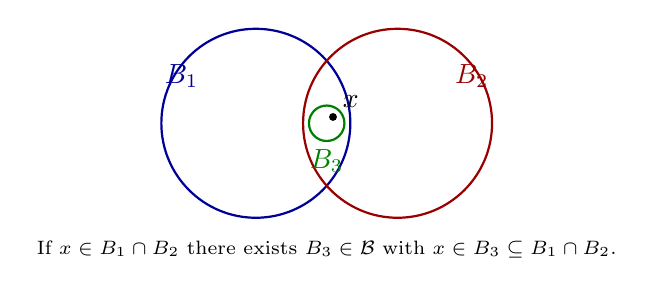
\begin{tikzpicture}[scale=1,baseline=(current bounding box.center)]
  % B1 and B2 (overlapping) - outlines only
  \draw[blue!60!black, thick] (-0.9,0) circle (1.2) node[left=6mm, yshift=6mm] {$B_1$};
  \draw[red!60!black, thick]  (0.9,0)  circle (1.2) node[right=6mm, yshift=6mm] {$B_2$};
  % B3 inside the intersection (smaller)
  \draw[green!50!black, thick] (0,0) circle (0.225) node[below=2mm] {$B_3$};
  % point x
  \filldraw[black] (0.08,0.08) circle (1.2pt) node[above right] {$x$};
  % optional intersection label
  \node at (0, -1.6) {\scriptsize If $x\in B_1\cap B_2$ there exists $B_3\in\mathcal B$ with $x\in B_3\subseteq B_1\cap B_2$.};
\end{tikzpicture}
\end{center}

\begin{example}
  Let $X$ be a metric space. Then, the collection of open balls forms a basis for the topology on $X$.
\end{example}

\begin{example}
  The collection of one point sets $\{ \{x\} : x\in X \}$ is a basis for the discrete topology on $X$.
\end{example}

\begin{example}
  Let ${\tau}$ be a topology on $X$. Then, $\mathcal{B}:={\tau}$ is a basis for ${\tau}$. This is a rather trivial case.
\end{example}

\begin{proposition}
  The topology generated by a basis is indeed a topology.
\end{proposition}
\begin{proof}
\begin{itemize}
  \item $\varnothing$ and $X$ are in ${\tau}_{\mathcal{B}}$: $\varnothing=\bigcup_{i\in\varnothing} B_i$ and $X=\bigcup_{x\in X} B_x$ where $B_x\in\mathcal{B}$ contains $x$.
  \item Arbitrary unions of sets in ${\tau}_{\mathcal{B}}$ belong to ${\tau}_{\mathcal{B}}$: Consider  $\{U_i\}_{i\in I}\subseteq{\tau}_{\mathcal{B}}$. Then, if $x\in \bigcup_{i\in I} U_i$, there exists $i_0\in I$ such that $x\in U_{i_0}$. Since $U_{i_0}$ is a union of basis elements, we can find $B\in\mathcal{B}$ with $x\in B\subseteq U_{i_0}$. Thus, $x\in B\subseteq \bigcup_{i\in I} U_i$. Hence, $\bigcup_{i\in I} U_i\in{\tau}_{\mathcal{B}}$.
  \item Now for $U_1,\ldots, U_n\in {\tau}_{\mathcal{B}}$, let $x\in U_1\cap\cdots\cap U_n$. We claim that there exists $B\in\mathcal{B}$ such that $x\in B\subseteq U_1\cap\cdots\cap U_n$. We prove by induction on $n$. The case $n=1$ is trivial. Assume the claim holds for $n=k$. Now consider $n=k+1$. By the induction hypothesis, there exists $B'\in\mathcal{B}$ such that $x\in B'\subseteq U_1\cap\cdots\cap U_k$. Since $U_{k+1}$ is open, there exists $B''\in\mathcal{B}$ such that $x\in B''\subseteq U_{k+1}$. Now, by the definition of basis, there exists $B\in\mathcal{B}$ such that $x\in B\subseteq B'\cap B''$. Hence, $x\in B\subseteq B'\cap B'' \subseteq (U_1\cap\cdots\cap U_k)\cap U_{k+1}=U_1\cap\cdots\cap U_{k+1}$. This proves the claim for $n=k+1$ and hence for all $n$.
\end{itemize}  
\end{proof}

\begin{proposition}
Let $(X,{\tau})$ be a topological space and let $\mathcal{B}\subset {\tau}$. Assume that for any $x\in U$ where $U\in {\tau}$, there exists $B\in\mathcal{B}$ with $x\in B\subseteq U$. Then $\mathcal{B}$ is a basis for ${\tau}$.
\end{proposition}
\begin{proof}
By hypothesis, for any open $U\in\tau$ and any $x\in U$ there exists $B\in\mathcal{B}$ with $x\in B\subseteq U$.

(1) Take $U=X\in\tau$. Then for every $x\in X$ there is $B\in\mathcal{B}$ with $x\in B\subseteq X$, verifying the first basis axiom.

(2) If $x\in B_1\cap B_2$ with $B_1,B_2\in\mathcal{B}\subseteq\tau$, then $U:=B_1\cap B_2\in\tau$. Applying the hypothesis to $U$ and $x$ yields $B_3\in\mathcal{B}$ such that $x\in B_3\subseteq B_1\cap B_2$, which is the second basis axiom.

Thus $\mathcal{B}$ is a basis. Let $\tau_{\mathcal{B}}$ be the topology it generates. Since $\mathcal{B}\subseteq\tau$ and $\tau$ is closed under unions, $\tau_{\mathcal{B}}\subseteq\tau$. Conversely, for any $U\in\tau$,
\[
U=\bigcup_{x\in U} B_x
\]
where each $B_x\in\mathcal{B}$ satisfies $x\in B_x\subseteq U$ by the hypothesis. Hence $U\in\tau_{\mathcal{B}}$, so $\tau\subseteq\tau_{\mathcal{B}}$. Therefore $\tau=\tau_{\mathcal{B}}$, and $\mathcal{B}$ is a basis for $\tau$.
\end{proof}

\begin{proposition}[Comparing topologies via bases]
Let $\mathcal{B}_1,\mathcal{B}_2$ be bases on $X$ generating ${\tau}_1,{\tau}_2$. Then ${\tau}_1\subseteq{\tau}_2$ iff for every $x\in X$ and $B_1\in\mathcal{B}_1$ with $x\in B_1$ there exists $B_2\in\mathcal{B}_2$ with $x\in B_2\subseteq B_1$.
\end{proposition}
\begin{proof}
($\Rightarrow$) If $B_1\in\mathcal{B}_1$, then $B_1\in{\tau}_1\subseteq{\tau}_2$ and so $B_1$ is a union of $\mathcal{B}_2$–elements. Pick one containing $x$ inside $B_1$.

($\Leftarrow$) Let $U\in{\tau}_1$; write $U=\bigcup_{i} B_i$ with $B_i\in\mathcal{B}_1$. For $x\in U$ choose $i$ with $x\in B_i$ and then $B_2\in\mathcal{B}_2$ with $x\in B_2\subseteq B_i\subseteq U$. Hence $U$ is open in ${\tau}_2$ by the basis criterion.
\end{proof}

\begin{example}
  Let $X=\R^2$. Let $\mathcal{B}=\{\text{open balls in }\R^2\}$ and let $\mathcal{B}'=\{\text{axis-aligned open rectangles in }\R^2\}$. Then they generate the same topology.
\begin{center}
  \begin{tikzcd}[column sep=12mm]
  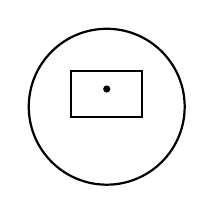
\begin{tikzpicture}[baseline=(current bounding box.center),scale=0.9]
    \draw[thick] (0,0) circle (1.1);
    \draw[thick] (-0.5,0.5) rectangle (0.5,-0.15);
    \filldraw[black] (0.0,0.25) circle (1.2pt);
  \end{tikzpicture}
  &
  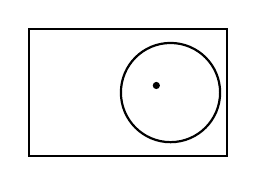
\begin{tikzpicture}[baseline=(current bounding box.center),scale=0.9]
    \draw[thick] (-1.4,-0.9) rectangle (1.4,0.9);
    \draw[thick] (0.6,0) circle (0.7);
    \filldraw[black] (0.4,0.1) circle (1.2pt);
  \end{tikzpicture}
  \end{tikzcd}
\end{center}
  
\end{example}

\subsubsection{Subbasis}

Now consider the case where we are just give a set of subsets, can we still generate a topology?

\begin{definition}[Subbasis]
A \emph{subbasis} $\mathcal{S}$ for a topology on $X$ is a collection of subsets whose union is $X$. The topology \emph{generated} by $\mathcal{S}$ is the collection of all unions of finite intersections of members of $\mathcal{S}$:
\[
{\tau}_{\mathcal{S}}=\Big\{\bigcup_{\alpha} \bigcap_{k=1}^{n_\alpha} S_{\alpha,k} : S_{\alpha,k}\in\mathcal{S},\ n_\alpha\ge 0\Big\}.
\]
\end{definition}

\begin{example}
  $\mathcal{S}=\{\{0,1\},\{0,2\}\}$ is a subbasis on $X=\{0,1,2\}$. It is clear that $\mathcal{S}$ is not a basis. The topology generated by $\mathcal{S}$ is ${\tau}_{\mathcal{S}}=\{\emptyset,\{0\},\{0,1\},\{0,2\},X\}$ with a basis $\{\{0\},\{0,1\},\{0,2\}\}$.
\end{example}

\begin{theorem}
  ${\tau}_{\mathcal{S}}$ is a topology on $X$ with the family of all finite intersections of members of $\mathcal{S}$ being a basis.
\end{theorem}
\begin{proof}
  Let $\mathcal{B}$ be the family of all finite intersections of members of $\mathcal{S}$. We first show that $\mathcal{B}$ is a basis. 

  \begin{itemize}
    \item For any $x\in X$, since $\bigcup_{S\in\mathcal{S}} S = X$, there exists $S\in\mathcal{S}$ such that $x\in S$. Hence, $x\in S\in\mathcal{B}$.
    \item For any $B_1=\bigcap_{i=1}^m S_i$ and $B_2=\bigcap_{j=1}^n S'_j$ in $\mathcal{B}$, we have that $B_1\cap B_2 = \bigcap_{i=1}^m S_i \cap \bigcap_{j=1}^n S'_j = \bigcap_{k=1}^{m+n} S_k\in \mathcal{B}$ for some $S_k\in\mathcal{S}$.
  \end{itemize}
  Then, it follows from the definition of $\tau_\mathcal{S}$ that ${\tau}_{\mathcal{S}}={\tau}_{\mathcal{B}}$.
\end{proof}

\begin{remark}
  ${\tau}_{\mathcal{S}}$ is the smallest topology containing $\mathcal{S}$, i.e., any other topology on $X$ containing $\mathcal{S}$ must also contain ${\tau}_{\mathcal{S}}$.
\end{remark}

\begin{example}
In $\R$ the open intervals $(a,b)$ form a basis. The family $\{(-\infty,a), (a,\infty): a\in\R\}$ is a subbasis generating the same topology.
\end{example}





\subsection{Kuratowski's approach}

As we've seen previously that the continuity of a function between metric spaces can be captured completely by closed sets and the notion of closure. This perspective resulted in the following definition of topology which is of course equivalent to the one given above.



\begin{definition}[Closure Operation]
Let \(X\) be a set and let
\[
\overline{\cdot} : \mathcal{P}(X) \to \mathcal{P}(X)
\]
be a map. It is called a \emph{closure operation} if for all \(A, B \subset X\):
\begin{enumerate}
  \item[(i)] \(\overline{\emptyset} = \emptyset\),
  \item[(ii)] \(A \subset \overline{A}\),
  \item[(iii)] If \(D = \overline{A}\), then \(\overline{D} = D\),
  \item[(iv)] \(\overline{A \cup B} = \overline{A} \cup \overline{B}\).
\end{enumerate}
\end{definition}

We now show that the closure operation and the topology we defined previously give rise to equivalent structures on a set. To this end, we identify the notion of a closed set in a topological space first.



\begin{proposition}
Given a topological space \((X, {\tau})\), define
\[
\overline{A} := \bigcap_{\substack{A \subset C \\ C \text{ closed}}} C.
\]
Then \(\overline{\cdot}\) is a closure operation in the sense of Definition 2.
\end{proposition}

\begin{proof}
\begin{itemize}
  \item[(i)] Since \(X\) is open, \(\emptyset\) is closed, so \(\overline{\emptyset} = \emptyset\).
  \item[(ii)] \(A\) is contained in every closed superset, so \(A \subset \overline{A}\).
  \item[(iii)] If \(D\) is closed and contains \(A\), then taking closure again yields \(D\) itself.
  \item[(iv)] For \(A,B \subset X\): $\overline{A}\cup\overline{B}$ is closed and it contains \(A \cup B\). Hence, \(\overline{A \cup B} \subseteq \overline{A} \cup \overline{B}\). Since $\overline{A}\subset \overline{A \cup B}$ and $\overline{B}\subset \overline{A \cup B}$, we conclude that \(\overline{A \cup B} = \overline{A} \cup \overline{B}\).
\end{itemize}
\end{proof}

\begin{proposition}
Conversely, if \(\overline{\cdot}\) is a closure operation as in Definition 2, then the sets
\[
\mathcal{C} := \{\overline{A} : A \subset X\}
\]
form the closed sets of a topology in the sense of Definition 1.
\end{proposition}

\begin{proof}
\begin{itemize}
  \item[(a)] From (i), \(\emptyset \in \mathcal{C}\); from (ii), \(X = \overline{X} \in \mathcal{C}\).
  \item[(b)] If \(\overline{A},\overline{B} \in \mathcal{C}\), then by (iii) and (iv), \(\overline{A} \cup \overline{B} = \overline{A \cup B} \in \mathcal{C}\). Inductively, one can show that finite unions of closed sets remain closed.
  \item[(c)] Now consider an arbitrary collection \(\{\overline{A_i}\}_{i \in I} \subseteq \mathcal{C}\). We first observe that if $A\subset B$ then $\overline{A}\subset \overline{B}$. This is due to the fact that $\overline{B}=\overline{A\cup B\setminus A}=\overline{A}\cup (B\setminus A)$. So for any $i\in I$, we have that $\overline{\bigcap_{i\in I} \overline{A_i}}\subset\overline{\overline{A}}_i=\overline{A}_i $. Therefore, \(\bigcap_{i\in I} \overline{A_i}\subseteq\overline{\bigcap_{i\in I} \overline{A_i}} \subseteq \bigcap_{i\in I} \overline{A_i}\). This implies that \(\bigcap_{i\in I} \overline{A_i} = \overline{\bigcap_{i\in I} \overline{A_i}} \in \mathcal{C}\).
\end{itemize}
\end{proof}

\subsubsection{Closure and Interior}

\begin{definition}[Interior]
Let \(X\) be a topological space and let \(A \subseteq X\). The \emph{interior} of \(A\), denoted \(\operatorname{int}(A)\) or \(\mathring{A}\), is the largest open set contained in \(A\). Equivalently, it is the union of all open sets contained in \(A\):
\[
\operatorname{int}(A) = \bigcup \{U \in \tau_X : U \subseteq A\}.
\]
\end{definition}

\begin{remark}
  For any subset $A\subset X$, we have that 
  \[
  \operatorname{int}(A) \subseteq A\subseteq \overline{A}.
  \]
\end{remark}

\begin{example}
  Let $X=\R$. Then, $\operatorname{int}((0,1]) = (0,1)$ and $\overline{(0,1]} = [0,1]$.
\end{example}

\begin{definition}
  Let $X$ be a topological space. For any $x\in X$, we say any open set containing $x$ is a \emph{(open) neighbourhood} of $x$.
\end{definition}

\begin{theorem}
  Let $X$ be a topological space and let $A\subseteq X$. Then,
  \begin{itemize}
    \item $x\in \overline{A}$ if and only if every neighbourhood of $x$ intersects $A$.
    \item $x\in \operatorname{int}(A)$ if and only if there exists a neighbourhood of $x$ contained in $A$.
  \end{itemize}
\end{theorem}

\begin{proof}
  The second item follows from the definition directly. We prove the first item below. 

  Let $x\in \overline{A}$. Assume that a neighborhood $U$ of $x$ does not intersect $A$. Then, $A\subseteq X\setminus U$. Notice that $X\backslash U$ is closed and contains $A$. Then, by definition of closure, we have $x\in \overline{A}\subseteq X\backslash U$, which is a contradiction. 

  Now, we assume $x\notin \overline{A}$. Then, there exists a closed set $C$ containing $A$ such that $x\notin C$. In particular, $x\in X\backslash C$. Note that $X\backslash C$ is open and $(X\setminus C)\cap A = \emptyset$.
\end{proof}

\newpage

\subsection{Order topology}

\begin{definition}[Linearly ordered set and intervals]
Let $(X,\le)$ be a linearly ordered (totally ordered) set. For $a,b\in X$ with $a<b$ define
\[
(a,b)=\{x\in X: a<x<b\},\quad
[a,b)=\{x\in X: a\le x<b\},
\]
\[
(a,b]=\{x\in X: a<x\le b\},\quad
[a,b]=\{x\in X: a\le x\le b\}.
\]
\end{definition}

\begin{definition}[Order topology]
Let $(X,\le)$ be a linearly ordered set with at least two elements. Let $\mathcal B$ be the family consisting of
\begin{itemize}
  \item all open intervals $(a,b)$ with $a<b$,
  \item all $[a_0,b)$ when $a_0$ is the least element of $X$ and $b>a_0$,
  \item all $(a,b_0]$ when $b_0$ is the greatest element of $X$ and $a<b_0$.
\end{itemize}
The topology generated by $\mathcal B$ is called the \emph{order topology} on $X$.
\end{definition}

\begin{proposition}
The family $\mathcal B$ above is a basis.
\end{proposition}
\begin{proof}
Nonemptiness is clear. Given $x\in X$, if $x$ is minimal, then $x$ is in $[x,b)$; if $x$ is maximal, then $x$ is in $(a,x]$; otherwise, there must exist $a,b$ such that $x\in (a,b)$. The intersection $B_1\cap B_2$ with $B_i\in\mathcal B$ must be one of the sets in $\mathcal{B}$ or emptyset.
\end{proof}

\begin{example}[Standard topology on $\R$]
With the usual order on $\R$, the sets $(a,b)$ already form $\mathcal B$, hence the order topology coincides with the usual metric topology on $\R$.
\end{example}

\begin{example}[Lexicographic order on $\R\times\R$]
Define $(x_1,y_1)<(x_2,y_2)$ iff $x_1<x_2$, or $x_1=x_2$ and $y_1<y_2$. The interval $((a,b),(c,d))$ looks like the following:


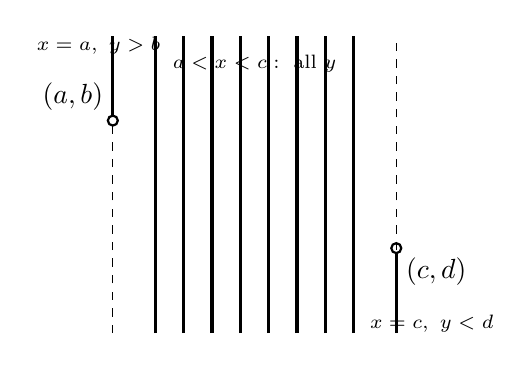
\begin{tikzpicture}[scale=0.9,baseline=(current bounding box.center)]
  % parameters
  \def\xA{0}
  \def\xC{4}
  \def\yB{1.0}
  \def\yD{-0.8}
  \def\Ymax{2.2}
  \def\Ymin{-2.0}

  % the strip a<x<c: every y is allowed (draw several full verticals)
  \foreach \x in {0.6,1.0,1.4,1.8,2.2,2.6,3.0,3.4}{
    \draw[very thick] (\x,\Ymin) -- (\x,\Ymax);
  }

  % boundary at x=a: only y>b (open at (a,b))
  \draw[very thick] (\xA,\yB) -- (\xA,\Ymax);
  \draw[fill=white,thick] (\xA,\yB) circle (2pt);
  \node[above left] at (\xA,\yB) {$(a,b)$};
  \draw[dashed] (\xA,\Ymin) -- (\xA,\Ymax);

  % boundary at x=c: only y<d (open at (c,d))
  \draw[very thick] (\xC,\Ymin) -- (\xC,\yD);
  \draw[fill=white,thick] (\xC,\yD) circle (2pt);
  \node[below right] at (\xC,\yD) {$(c,d)$};
  \draw[dashed] (\xC,\Ymin) -- (\xC,\Ymax);

  % annotations
  \node at (2.0,1.8) {\scriptsize $a<x<c:\ \text{all }y$};
  \node[above] at (-0.2,1.8) {\scriptsize $x=a,\ y>b$};
  \node[below] at (4.5,-1.6) {\scriptsize $x=c,\ y<d$};
\end{tikzpicture}

This is different from the standard topology on $\R^2$. In fact, the set above in the basis is not open in the standard topology. To see this, consider the point $(a,b+1)$ in the set. Any open ball around it will contain points with $x<a$, which are not in the set.
\end{example}

\begin{example}[Discrete order on the integers]
On $\mathbb{N}$ with the usual order, the order topology is discrete:
\[
\{n\}=(n-1,n+1)\quad\text{for }n>1;
\]
and $1$ is the least element then $\{1\}=[1,2)$. Hence every singleton is open.
\end{example}

\begin{example}[Order topology on $\{1,2\}\times\mathbb{N}$ (lexicographic) is not discrete]
Give $X=\{1,2\}\times\mathbb{N}$ the lexicographic order:
\[
(i,m)<(j,n)\quad\text{iff}\quad i<j\ \text{ or }\ (i=j\text{ and }m<n).
\]
Then $(1,1)$ is the least element. In the order topology, any basis element containing $(2,1)$ is of the form $(a,b)$ (or $[\, (1,1),b)$)
with $a<(2,1)<b$, and therefore must contain some $(1,n)$. Hence $\{(2,1)\}$ is not open, so the
order topology on $X$ is not the discrete topology.

% \begin{center}
% \begin{tikzpicture}[x=0.8cm,y=0.7cm,baseline=(current bounding box.center)]
%   % two rows of points: top is {2}xN, bottom is {1}xN
%   \foreach \k in {1,...,7}{
%     \fill (\k,0) circle (1.2pt);        % (2,k)
%     \fill (\k,-1.2) circle (1.2pt);     % (1,k)
%   }
%   % labels for a few points
%   \node[above] at (1,0) {\scriptsize $(2,1)$};
%   \node[above] at (2,0) {\scriptsize $(2,2)$};
%   \node[below] at (1,-1.2) {\scriptsize $(1,1)$};
%   \node[below] at (2,-1.2) {\scriptsize $(1,2)$};
%   \node at (7.8,-0.6) {\scriptsize $\cdots$};

%   % indicate a basic nbhd around (2,1) that must catch some (1,n)
%   \draw[thick,rounded corners,blue] (0.6,-0.35) rectangle (2.6,0.35);
%   \node[blue,above right] at (2.6,0.35) {\scriptsize neighborhood of $(2,1)$};
%   \draw[->,>=stealth,blue] (2.2,0.35) .. controls (1.9,-0.1) .. (1.6,-1.0);
%   \node[below,blue] at (1.6,-1.2) {\scriptsize some $(1,n)$};
% \end{tikzpicture}
% \end{center}
\end{example}



\subsection{Product Topology on $X\times Y$}

\begin{definition}
  Let $(X,{\tau}_X)$ and $(Y,{\tau}_Y)$ be topological spaces. The \emph{product topology} on the product space $X\times Y$ is the topology generated by the basis consisting of all products of open sets:
  \[
    \mathcal{B}_{X\times Y} = \{ U \times V : U \in {\tau}_X, V \in {\tau}_Y \}.
  \]
\end{definition}

\begin{proof}[Check: $\mathcal{B}$ is a basis]
  Note  $X\times Y\in \mathcal{B}$ so every point $(x,y)\in X\times Y$ lies in some basis element.

  For $U_1\times V_1,U_2\times V_2\in \mathcal{B}$, we have $U_1\cap U_2\in {\tau}_X$ and $V_1\cap V_2\in {\tau}_Y$, so
  \[
    (U_1\times V_1)\cap (U_2\times V_2) = (U_1\cap U_2)\times (V_1\cap V_2)\in \mathcal{B}.
  \]
\end{proof}

Question: is $\mathcal{B}$ a topology? No, the union of basis elements is not necessarily a basis element.

It turns out that smaller bases can also generate the product topology.

\begin{theorem}
  If $\mathcal{B}$ is a basis for ${\tau}_X$ and $\mathcal{B}'$ is a basis for ${\tau}_Y$, then
  \[
    \mathcal{B} \times \mathcal{B}' = \{ U \times V : U \in \mathcal{B}, V \in \mathcal{B}' \}
  \]
  is a basis for the product topology on $X \times Y$.
\end{theorem}
\begin{proof}
  Pick any $U\times V$ from the basis for the product topology. Now, for any $(x,y)\in U\times V$, we have that $x\in U$ and $y\in V$. Since $\mathcal{B}$ and $\mathcal{B}'$ are bases, there exist $U_x\in\mathcal{B}$ and $V_y\in\mathcal{B}'$ such that $x\in U_x\subseteq U$ and $y\in V_y\subseteq V$. Hence, $(x,y)\in U_x\times V_y \subseteq U\times V$. This implies that the topology generated by $\mathcal{B}\times\mathcal{B}'$ is finer than the product topology. On the other hand, since $\mathcal{B}\times\mathcal{B}'$ is a subset of the basis for the product topology, the topology generated by $\mathcal{B}\times\mathcal{B}'$ is coarser than the product topology. Therefore, they must be the same. 
\end{proof}

\begin{example}
  Let $X=Y=\R$ with the standard topology. Then, $\mathcal{B}=\{(a,b): a<b\}$ is a basis for $\R$. Hence, $\mathcal{B}\times\mathcal{B}=\{(a,b)\times(c,d): a<b, c<d\}$ is a basis for the product topology on $\R^2$. Note that $(a,b)\times(c,d)$ is an axis-aligned open rectangle in $\R^2$. Previously, we showed that this generates the same topology as the one generated by open balls in $\R^2$. So the product topology on $\R^2$ is the same as the standard metric topology on $\R^2$.
\end{example}

We can inductively define the product topology on $X_1\times X_2\times \cdots \times X_n$ for any finite $n$. But things will be a bit different for infinite products. We will discuss this later.

\begin{definition}
  Let $\pi_1:X\times Y\to X$ be defined by $\pi_1(x,y)=x$ and $\pi_2:X\times Y\to Y$ be defined by $\pi_2(x,y)=y$. The maps $\pi_1$ and $\pi_2$ are called the \emph{projections} of $X\times Y$ onto its first and second factors, respectively.
\end{definition}

Note that for any open set $U\subset X$, we have that $\pi_1^{-1}(U) = U\times Y$ and $\pi_2^{-1}(V) = X\times V$ for any open set $V\subset Y$.

\begin{theorem}
  The collection 
  \[\mathcal{S}=\{\pi_1^{-1}(U): U\in{\tau}_X\}\cup \{\pi_2^{-1}(V): V\in{\tau}_Y\}\]
  is a subbasis for the product topology on $X\times Y$.
\end{theorem}

\begin{proof}
  Note that for any $U\in\tau_X$ and $V\in\tau_Y$, we have that 
  \[U\times V = \pi_1^{-1}(U)\cap \pi_2^{-1}(V).\]
  Hence, the basis generated by $\mathcal{S}$ contains all basis elements of the product topology. On the other hand, elements in $\mathcal{S}$ are open in the product topology. Therefore, the topology generated by $\mathcal{S}$ is the same as the product topology. 
\end{proof}



\subsection{Subspace Topology}

\begin{definition}
  Suppose $(X,{\tau})$ is a topological space and let $A$ be a subset of $X$. The \emph{subspace topology} on $A$ is the collection ${\tau}_A := \{ U \cap A : U \in {\tau} \}$. Then $(A,{\tau}_A)$ is a topological space.
\end{definition}

We now check that ${\tau}_A$ is indeed a topology on $A$.
\begin{itemize}
  \item $\varnothing$ and $A$ are in ${\tau}_A$: $\varnothing = \varnothing \cap A$ and $A = X \cap A$.
  \item Arbitrary unions of sets in ${\tau}_A$ belong to ${\tau}_A$: If $\{U_i \cap A\}_{i \in I} \subseteq {\tau}_A$, then
  \[
    \bigcup_{i \in I} (U_i \cap A) = \Big(\bigcup_{i \in I} U_i\Big) \cap A \in {\tau}_A.
  \]
  \item Finite intersections of sets in ${\tau}_A$ belong to ${\tau}_A$: If $U_1 \cap A,\ldots, U_n \cap A \in {\tau}_A$, then
  \[
    (U_1 \cap A) \cap\ldots\cap (U_n \cap A) = (U_1 \cap \ldots\cap U_n) \cap A \in {\tau}_A.
  \]
\end{itemize}

\begin{example}
  $[0,1]$ is a subspace of $\mathbb{R}$. Note that $(0.5,1]$ is not open in $\R$ but open in $[0,1]$ with the subspace topology as $$(0.5,1] = (0.5,2) \cap [0,1]$$
\end{example}

\begin{lemma}
Let $(X,{\tau})$ be a topological space and $Y\subseteq X$. If $Y\in{\tau}$ and $U\in{\tau}_Y$ (i.e.\ $U$ is open in the subspace $Y$), then $U\in{\tau}$.
\end{lemma}
\begin{proof}
By definition of the subspace topology, $U\in{\tau}_Y$ means there exists $V\in{\tau}$ with $U=V\cap Y$. Since $Y\in{\tau}$ and ${\tau}$ is closed under finite intersections, $U=V\cap Y$ is open in $X$. Hence $U\in{\tau}$.
\end{proof}

\begin{lemma}
Let $(X,{\tau})$ be a topological space and let $\mathcal{B}$ be a basis for ${\tau}$. If $Y\subseteq X$ then
\[
\mathcal{B}_Y:=\{\,B\cap Y : B\in\mathcal{B}\,\}
\]
is a basis for the subspace topology ${\tau}_Y$ on $Y$.
\end{lemma}
\begin{proof}
  Given any $U\cap Y$ open ($U$ is open in $X$) in $Y$ and $y\in U\cap Y$, there exists $B\in\mathcal{B}$ such that $y\in B\subseteq U$. Then, $y\in B\cap Y\subseteq U\cap Y$. Thus, $\mathcal{B}_Y$ is a basis for $\tau_Y$.
\end{proof}

\subsubsection*{Order topology versus subspace topology}

\begin{theorem}
  If $A\subseteq X$ and $B\subseteq Y$, then the product topology on $A\times B$ is the same as the subspace topology inherited from $X\times Y$.
\end{theorem}
\begin{proof}
  Let $\mathcal{B}_X$ and $\mathcal{B}_Y$ be bases for $X$ and $Y$ respectively. Then, $\mathcal{B}_X\times \mathcal{B}_Y:=\{U\times V: U\in\mathcal{B}_X, V\in\mathcal{B}_Y\}$ is a basis for the product topology on $X\times Y$. Hence, the subspace topology of $A\times B$ has a basis
  \[\mathcal{B}_{A\times B}=\{(U\times V)\cap (A\times B): U\in\mathcal{B}_X, V\in\mathcal{B}_Y\}.\]
  Note that $(U\times V)\cap (A\times B) = (U\cap A)\times (V\cap B)$. 

  Then,
  \[
  \mathcal{B}_{A\times B}=\{(U\cap A)\times (V\cap B): U\in\mathcal{B}_X, V\in\mathcal{B}_Y\}=\mathcal{B}_A\times \mathcal{B}_B.
  \]
  This finishes the proof.
\end{proof}



\begin{theorem}
  Let $(X,d)$ be a metric space and let $Y\subseteq X$. Consider the sub metric space $(Y,d_Y)$. Then, the topology induced by $d_Y$ is the same as the subspace topology inherited from $(X,d)$.
\end{theorem}
\begin{proof}
  Let $\tau_{d_Y}$ be the topology induced by $d_Y$, and let $\tau_Y$ be the subspace topology on $Y$ inherited from the topology induced by $d$.

  Suppose first that $U\in\tau_{d_Y}$. For every $y\in U$, there exists $r>0$ such that $B_r^Y(y)\subseteq U$. Since
  \[
    B_r^Y(y)=B_r^X(y)\cap Y,
  \]
  the set $B_r^Y(y)$ is open in the subspace topology. Thus every point of $U$ has a $\tau_Y$-open neighborhood contained in $U$, so $U\in\tau_Y$.

  Conversely, suppose that $U\in\tau_Y$. Then $U=V\cap Y$ for some open set $V$ in $(X,d)$. For every $y\in U$, there exists $r>0$ such that $B_r^X(y)\subseteq V$. Hence
  \[
    B_r^Y(y)=B_r^X(y)\cap Y\subseteq V\cap Y=U.
  \]
  Therefore $U$ is open in $(Y,d_Y)$, so $U\in\tau_{d_Y}$. We conclude that $\tau_{d_Y}=\tau_Y$.
\end{proof}




Although the subspace topology and the metric topology are compatible, the order topology and the subspace topology are not always compatible. We will see when they agree.

\begin{remark}
The order and subspace topologies on a subset of a linearly ordered set need not agree.  
For instance, let \(Y=[0,1)\cup\{2\}\subset\R\) with the induced order.  
In the subspace topology, \(\{2\}\) is open in \(Y\) since \(\{2\}=(2-\tfrac12, 2+\tfrac12) \cap Y\).  
But in the order topology on \(Y\), any basis element containing \(2\) is of the form
\((a,2]_Y=\{y\in Y:a<y\le 2\}\) where $a\in Y$ (because \(2\) is the greatest element of \(Y\)),  
so it contains points of \(Y\) strictly less than \(2\); hence \(\{2\}\) is not open there.
\end{remark}

\begin{definition}[Convex subset]
Let \((X,\le)\) be a linearly ordered set. A subset \(Y\subset X\) is \emph{convex} if for all
\(a,b\in Y\) with \(a<b\) one has \((a,b)_X\subset Y\).
\end{definition}

\begin{theorem}
Let \(X\) be a linearly ordered set with the order topology, and let \(Y\subset X\) be convex (with the induced order). Then the order topology on \(Y\) coincides with the subspace topology inherited from \(X\).
\end{theorem}

For a proof, see Munkres, Theorem 16.4.
%%%%%%%%%%

\subsection{Continuous functions}

Now we consider the functions between two topological spaces.

We first define the continuity using a local idea adopted from metric spaces. Then, we will see some more global characterizations.
\begin{definition}
  A function $f:(X,{\tau}_X)\to(Y,{\tau}_Y)$ between topological spaces is called \emph{continuous} at a given point $x\in X$ if for every neighbourhood $V$ of $f(x)$ in $Y$, there exists a neighbourhood $U$ of $x$ in $X$ such that $f(U)\subseteq V$. We say that $f$ is \emph{continuous} if it is continuous at every point $x\in X$.
\end{definition}







\begin{example}
  A function $f:X\to Y$ between two metric spaces is continuous in the metric sense if and only if it is continuous in the topological sense.
\end{example}

\begin{theorem}
  Let $X$ and $Y$ be topological spaces and let $f:X\to Y$ be a function. The following are equivalent:
  \begin{enumerate}
    \item $f$ is continuous.
    \item For all open sets $H$ in $Y$, $f^{-1}(H)$ is open in $X$.
    \item For all closed sets $C$ in $Y$, $f^{-1}(C)$ is closed in $X$.
    \item For all $A\subset X$, $f(\overline{A}) \subseteq \overline{f(A)}$ (This can be thought of as the Kuratowski definition of continuity).
  \end{enumerate}
\end{theorem}

\begin{proof}

We are going to use the following observation several times:
For any $A\subseteq Y$, we have that 
\[X=f^{-1}(A)\cup f^{-1}(Y\setminus A).\]

  $(1)\Rightarrow(2)$: Let $H$ be open in $Y$. If $f^{-1}(H)=\emptyset$, then done. Otherwise, for any $x\in f^{-1}(H)$, $H$ is a neighborhood of $f(x)$. Hence, there exists a neighborhood $V$ of $x$ such that $f(V)\subseteq H$. Thus, $V\subseteq f^{-1}(H)$. Therefore, $f^{-1}(H)$ is open in $X$.

  $(2)\Rightarrow(3)$: If $C$ is closed in $Y$, then $Y\setminus C$ is open in $Y$. By (2), $f^{-1}(Y\setminus C)$ is open in $X$. Then, $f^{-1}(C)=X\setminus f^{-1}(Y\setminus C)$ is closed in $X$.

  $(3)\Rightarrow(4)$: $f^{-1}(\overline{f(A)})$ is closed by (2). Furthermore, $A\subseteq f^{-1}(\overline{f(A)})$ (since $f(A)\subseteq \overline{f(A)}$). This implies that $\overline{A} \subseteq f^{-1}(\overline{f(A)})$ and hence $f(\overline{A}) \subseteq \overline{f(A)}$.

  $(4)\Rightarrow(1)$: Let $x\in X$ and let $V$ be a neighborhood of $f(x)$ in $Y$. Set $E:=f^{-1}(Y\setminus V)=X\setminus f^{-1}(V)$. Then, we have that $f(\overline{E})\subset \overline{f(E)}\subseteq Y\setminus V$ (because $Y\setminus V$ is a closed set containing $f(E)$).

  Now we have that $x\in X\setminus \overline{E}$, which is a neighborhood of $x$. Then,
  \begin{align*}
    f(X\setminus \overline{E})\subset f(X\setminus E)=f(X\setminus f^{-1}(Y\setminus V))=f(f^{-1}(V))\subseteq V.
  \end{align*}
  This concludes the proof.
\end{proof}



\begin{remark}
  A function $f:(X,{\tau}_X)\to(Y,{\tau}_Y)$ is continuous if and only if the statement (2) holds  for all basis elements of $Y$:

  \[U=\cup B_\alpha\quad f^{-1}(U)=\cup f^{-1}(B_\alpha)\]
  \end{remark}
  
  
  \begin{remark}
  A function $f:(X,{\tau}_X)\to(Y,{\tau}_Y)$ is continuous if and only if the statement (2) holds  for all subbasis elements of $Y$:

  \[B=S_1\cap\cdots\cap S_n\quad f^{-1}(B)=\cap f^{-1}(S_i)\]
\end{remark}

\begin{remark}
  In some books, they take the (2) as the definition of continuity.
\end{remark}


\begin{example}
  Let \(f:\R\to\R\) be the constant map \(f(x)=0\). Then \(f\) is continuous, but the image of the open set \((0,1)\) is
  \[
    f((0,1))=\{0\},
  \]
  which is not open in \(\R\). Thus a continuous map need not send open sets to open sets.
\end{example}

\begin{example}
  Let $\pi:\R^2\to\R$ be the projection $\pi(x,y)=x$, which is continuous. Consider
  \[
    C=\{(x,y)\in\R^2: xy=1\},
  \]
  the hyperbola. Since $C$ is the zero set of the continuous function $f:(x,y)\mapsto xy-1$, it is closed in $\R^2$ (i.e., $C=f^{-1}(\{0\})$). But
  \[
    \pi(C)=\{x\in\R:x\neq0\}=\R\setminus\{0\},
  \]
  which is not closed in $\R$. Thus a continuous map need not send closed sets to closed sets.
\end{example}

\begin{example}
  Let $X\times Y$ be endowed with the product topology. Then, $\pi_X:X\times Y\to X$ and $\pi_Y:X\times Y\to Y$ are continuous.

  Note that for any open set $U$ in $X$, $\pi_X^{-1}(U)=U\times Y$ is open in $X\times Y$. Similarly, for any open set $V$ in $Y$, $\pi_Y^{-1}(V)=X\times V$ is open in $X\times Y$.

  Note also that the product topology $\tau_{X\times Y}$ is the smallest topology on $X\times Y$ such that both $\pi_X$ and $\pi_Y$ are continuous: any topology on $X\times Y$ that makes both $\pi_X$ and $\pi_Y$ continuous must contain a basis for $\tau_{X\times Y}$: sets of the form $U\times Y$ and $X\times V$ for all open sets $U$ in $X$ and $V$ in $Y$. 
\end{example}

\subsubsection{Constructing continuous functions}
\begin{theorem}
  \begin{enumerate}
    \item (Constant function) If $f:X\to Y$ maps all of $X$ to a single point $y_0\in Y$, then $f$ is continuous.
    \item (Inclusion) If $A$ is a subspace of $X$, the inclusion map $i:A\to X$ defined by $i(a)=a$ is continuous.
    \item (Composition) If $f:X\to Y$ and $g:Y\to Z$ are continuous, then the composition $g\circ f:X\to Z$ is continuous.
    \item (Restricting the domain) If $f:X\to Y$ is continuous and $A\subseteq X$, then the restriction $f|_A:A\to Y$ defined by $f|_A(a)=f(a)$ is continuous.
    \item (Restricting or expanding the range) Let $f:X\to Y$ be continuous. If $f(X)\subset Z\subset Y$, then the function $g:X\to Z$  obtained by restricting the range of $f$ is continuous. If $Y\subset W$, then the function $h:i_{Y\to W}\circ f:X\to W$ is continuous.
    \item (Local formulation) $f:X\to Y$ is continuous if $X=\cup U_\alpha$ for a family of open sets $U_\alpha$ and each restriction $f|_{U_\alpha}$ is continuous.
    \item (Pasting lemma) If $X=A\cup B$ with $A,B$ closed, and $f:A\to Y$, $g:B\to Y$ are continuous and agree on $A\cap B$ (i.e., $f(x)=g(x)$ for all $x\in A\cap B$), then the function $h:X\to Y$ defined by
    \[h(x)=\begin{cases}
    f(x),&x\in A\\
    g(x),&x\in B
    \end{cases}\]
    is continuous.
  \end{enumerate}
\end{theorem}

\begin{proof}
  \begin{enumerate}
    \item For any open set $U$ in $Y$, if $y_0\in U$, then $f^{-1}(U)=X$; otherwise, $f^{-1}(U)=\emptyset$. In both cases, $f^{-1}(U)$ is open in $X$. Hence, $f$ is continuous.
    \item For any open set $U$ in $X$, $i^{-1}(U)=U\cap A$ is open in $A$. Hence, $i$ is continuous.
    \item For any open set $W$ in $Z$, $(g\circ f)^{-1}(W)=f^{-1}(g^{-1}(W))$. Since $g$ is continuous, $g^{-1}(W)$ is open in $Y$. Since $f$ is continuous, $f^{-1}(g^{-1}(W))$ is open in $X$. Hence, $g\circ f$ is continuous.
    \item For any open set $U$ in $Y$, $(f|_A)^{-1}(U)=f^{-1}(U)\cap A$ is open in $A$. Hence, $f|_A$ is continuous.
    \item For any open set $V$ in $Z$, then there exists $U$ open in $Y$ such that $V=U\cap Z$. Hence, $g^{-1}(V)=f^{-1}(V)=f^{-1}(U\cap Z)$. Since $f(X)\subset Z$, we have that $f^{-1}(U\cap Z)=f^{-1}(U)$ is open in $X$. Hence, $g$ is continuous. The continuity of $h$ follows from 2 and 3.
    \item For any open set $U$ in $Y$, we first note that 
    \[f^{-1}(U)\cap U_\alpha=(f|_{U_\alpha})^{-1}(U)=\{x\in U_\alpha: f(x)\in U\}.\]
    Since $f|_{U_\alpha}$ is continuous, $(f|_{U_\alpha})^{-1}(U)$ is open in $U_\alpha$. Hence,
    \[f^{-1}(U)=\bigcup (f^{-1}(U)\cap U_\alpha)=\bigcup (f|_{U_\alpha})^{-1}(U)\] is open in $X$. This shows that $f$ is continuous.
    \item For any closed set $C$ in $Y$, $h^{-1}(C)=f^{-1}(C)\cup g^{-1}(C)$. Since $A$ and $B$ are closed, $f^{-1}(C)$ and $g^{-1}(C)$ are closed in $X$ (see the later lemma for this). Hence, $h^{-1}(C)$ is closed in $X$. This shows that $h$ is continuous.
    \begin{lemma}
  Let $A\subset X$ and let $E\subset A$. Then, $E$ is closed in $A$ if and only if there exists a closed set $F$ in $X$ such that $E=F\cap A$.
\end{lemma}
\begin{proof}
  Suppose $E$ is closed in $A$. Then $A \setminus E$ is open in $A$, so there exists an open set $U$ in $X$ such that $A \setminus E = U \cap A$. Let $F = X \setminus U$, which is closed in $X$. Then
  \[
  F \cap A = (X \setminus U) \cap A = A \setminus (U \cap A) = A \setminus (A \setminus E) = E.
  \]

  Conversely, if $E = F \cap A$ for some closed set $F$ in $X$, then
  \[
  A \setminus E = A \setminus (F \cap A) = A \cap (X \setminus F),
  \]
  where $X \setminus F$ is open in $X$. Hence, $A \setminus E$ is open in $A$, so $E$ is closed in $A$.
\end{proof}
\begin{corollary}
  Let $A\subset X$ and let $E\subset A$. If $E$ is closed in $A$ then $E$ is closed in $X$.
\end{corollary}
\begin{proof}
  Since $E$ is closed in $A$, there exists a closed set $F$ in $X$ such that $E=F\cap A$. Since $A\subset X$ is closed, we have that $E$ is closed in $X$
\end{proof}
  \end{enumerate}
\end{proof}
  


\begin{remark}
  7 is the closed set and finite version of 6. See your homework for the infinite version of 7.
\end{remark}

\begin{theorem}
  Let $f:A\to X\times Y$ be given by $f(a)=(f_X(a),f_Y(a))$. Then $f$ is continuous if and only if $f_X$ and $f_Y$ are continuous.
\end{theorem}
\begin{proof}
  Recall the projections $\pi_X:X\times Y\to X$ and $\pi_Y:X\times Y\to Y$. Note that $f_X=\pi_X\circ f$ and $f_Y=\pi_Y\circ f$. 

  $\Rightarrow$: If $f$ is continuous, then $f_X$ and $f_Y$ are continuous by the composition of continuous functions.

  $\Leftarrow$: For $U\times V$ a basis element in $X\times Y$, we have that
  \[f^{-1}(U\times V) = f^{-1}(\pi_X^{-1}(U)\cap \pi_Y^{-1}(V)) = f^{-1}(\pi_X^{-1}(U))\cap f^{-1}(\pi_Y^{-1}(V)) = f_X^{-1}(U)\cap f_Y^{-1}(V).\]
  Since $f_X$ and $f_Y$ are continuous, $f^{-1}(U\times V)$ is open in $A$. This shows that $f$ is continuous.
\end{proof}


\subsubsection{Homeomorphism}
\begin{definition}
  A function \(f: X \to Y\) between topological spaces is a \emph{homeomorphism} if it is a bijection and both \(f\) and \(f^{-1}\) are continuous. 

  If $f$ is not surjective, we let $Z=f(X)$. If the restriction $f':X\to Z$ is a homeomorphism, then we say that $f$ is a topological embedding of $X$ into $Y$.
\end{definition}

Homeomorphisms preserve topological properties, meaning that if \(X\) and \(Y\) are homeomorphic, they share all topological characteristics. More precisely, we have the following theorem.

\begin{theorem}
  Let $f:X\to Y$ be a homeomorphism. Then, $f$ induces a map $f_*:\tau_X\to\tau_Y$ defined by $f_*(U)=f(U)$ for all $U\in\tau_X$. Furthermore, $f_*$ is a bijection.
\end{theorem}
\begin{proof}
  For any $U\in\tau_X$, $f(U)=(f^{-1})^{-1}(U)$. Since $f^{-1}$ is continuous, $f(U)$ is open in $Y$. This shows that $f_*$ is well-defined.

  Next, we show that $f_*$ is injective. If $f_*(U_1)=f_*(U_2)$ for some $U_1,U_2\in\tau_X$, then $f(U_1)=f(U_2)$. Since $f$ is bijective, we have that $U_1=U_2$. This shows that $f_*$ is injective.

  Finally, we show that $f_*$ is surjective. For any $V\in\tau_Y$, since $f^{-1}$ is continuous, we have that $f^{-1}(V)$ is open in $X$. Then, 
  \[
    f_*(f^{-1}(V))=f(f^{-1}(V))=V.
  \]
  This shows that $f_*$ is surjective.

  Therefore, we conclude that $f_*:\tau_X\to\tau_Y$ is a bijection.
\end{proof}

\begin{example}
  Suppose you have a subspace in some ambient Euclidean space. You can stretch and bend it without tearing or gluing. This is a homeomorphism. For example, a coffee cup is homeomorphic to a donut (solid torus).
\end{example}

\begin{example}
  The circle and the trefoil knot are homeomorphic. But we can't deform one to the other in 3D space without cutting. 
\end{example}

\begin{example}
  The map $f:(-1,1)\to \R$ defined by $f(x)=\frac{x}{1-x^2}$ is a homeomorphism with inverse $f^{-1}: \R \to (-1,1)$ given by $f^{-1}(y)=\frac{2y}{1+\sqrt{1+4y^2}}$. So homeomorphisms need not preserve boundedness. 
\end{example}


\begin{example}[Continuous bijection not a homeomorphism]
Let
\[
X = [0, 1)
\]
with the usual topology from $\mathbb{R}$, and
\[
Y = S^1 = \{ (x,y) \in \mathbb{R}^2 : x^2 + y^2 = 1 \}
\]
with the subspace topology from $\mathbb{R}^2$.

Define
\[
f: X \to Y, \quad f(t) = (\cos 2\pi t, \sin 2\pi t).
\]
Then $f$ is a continuous bijection. However, $f^{-1}$ is not continuous: around $(1, 0) \in S^1$, neighborhoods correspond to $t$ near $0$ \emph{and} near $1$,  
  which are far apart in $[0,1)$, so $f^{-1}$ fails continuity there.

\noindent
This shows that a continuous bijection need not be a homeomorphism when the domain is not compact.
\end{example}


\begin{example}
  Is $(0,1)$ homeomorphic to $[0,1)$?
\end{example}

\begin{lemma}
  Let $f:X \to Y$ be a homeomorphism. Let $x_0\in X$. Then, the map $g:X\setminus \{x_0\} \to Y \setminus \{f(x_0)\}$ defined by $g(x) = f(x)$ is also a homeomorphism.
\end{lemma}

\begin{definition}
  Let $X$ be a topological space. We say $X$ is connected if it cannot be represented as the union of two disjoint non-empty open sets. 
\end{definition}

\begin{remark}
  If $X$ is connected and $X$ is homeomorphic to $Y$, then $Y$ is also connected. This holds obviously as the homeomorphism gives rise to a bijection between the topologies.
\end{remark}

Now we are ready to answer the previous question.

\begin{theorem}
  $(0,1)$ is not homeomorphic to $[0,1)$.
\end{theorem}
\begin{proof}
  Suppose there exists a homeomorphism $f:[0,1)\to(0,1)$. Pick any $x_0=0$ and consider the map $g:(0,1)\to(0,1)\setminus\{f(x_0)\}$ defined by $g(x)=f(x)$. By the previous lemma, $g$ is a homeomorphism. 
  Note that $(0,1)\setminus\{f(x_0)\}$ is not connected regardless the value of $f(x_0)$. However, $(0,1)=[0,1)\setminus\{x_0\}$ is connected. This is a contradiction.
\end{proof}

\begin{example}
  Similarly, we can prove that $\R$ and $\R^2$ are not homeomorphic. 
  
  How about $\R^2$ vs $\R^3$? Need algebraic topology. We will have a taste of it later in the course.
\end{example}


\subsection{Product Topology}

Recall the Cartesian product of a family of sets $\{X_i\}_{i\in I}$ is the set of functions:

\[
\prod_{i\in I} X_i := \{ x:I\to \cup_{i\in I} X_i | \text{ for all } i\in I, x(i)\in X_i \}.
\]

Let's mimic the case when $I$ is a two-point set to identify the following definition of topology.

\begin{definition}[Box topology (less important)]
For spaces $(X_i,{\tau}_i)$, $i\in I$, the \emph{box topology} on $\prod_{i\in I}X_i$ is generated by the basis
\[
\mathcal{B}_{\text{box}}=\Big\{\prod_{i\in I}U_i : U_i\in{\tau}_i\text{ for every }i\Big\}
\]
\end{definition}

Let's first verify that $\mathcal{B}_{\text{box}}$ is indeed a basis. For any $x\in \prod_{i\in I} X_i$, we have that $x\in \prod_{i\in I} X_i = \prod_{i\in I} X_i$. Furthermore, for any two basis elements $\prod_{i\in I} U_i$ and $\prod_{i\in I} V_i$, we have that
\[x\in \prod_{i\in I} (U_i\cap V_i) =\prod_{i\in I} U_i \cap \prod_{i\in I} V_i.\]
Since $U_i$ and $V_i$ are open in $X_i$, $U_i\cap V_i$ is open in $X_i$. This shows that $\mathcal{B}_{\text{box}}$ is indeed a basis.

This basis seems reasonable right? But this topology is too fine and makes many things not work. 

\begin{example}
Let $X=\R^{\N}=\prod_{n\ge1}\R$. Then, the ``diagonal'' map $f:\R\to X$ defined by $f(t)=(t,t,t,\ldots)$ is not continuous when $X$ is endowed with the box topology. Consider the open set $(-1,1)\times (-1/2,1/2)\times (-1/3,1/3)\times \cdots$. Then, 
\begin{align*}
&f^{-1}((-1,1)\times (-1/2,1/2)\times (-1/3,1/3)\times \cdots)\\
 &= f^{-1}((-1,1)\times\R\times\cdots\cap\R\times (-1/2,1/2)\times\R\times\cdots\cap\cdots)\\
&=\bigcap_{n\ge1} f^{-1}(\R\times\cdots\times (-1/n,1/n)\times \cdots)\\
&=\bigcap_{n\ge1} (-1/n,1/n) = \{0\}.
\end{align*}
Then $f^{-1}((-1,1)\times (-1/2,1/2)\times (-1/3,1/3)\times \cdots)$ is not open in $\R$. Hence, $f$ is not continuous.

\end{example}

This example actually gives us a hint how we can make things right. The problem above is that when considering the arbitrary intersection of open sets, we don't get an open set. SO, we want things to be finite in some sense. This leads to the following definition.

\begin{definition}[Product topology]
For spaces $(X_i,{\tau}_i)$, $i\in I$, the \emph{product} $X=\prod_{i\in I} X_i$ carries the product topology generated by the basis
\[
\mathcal{B}_{\text{prod}}=\Big\{\prod_{i\in I} U_i : U_i\in{\tau}_i \text{ and } U_i=X_i \text{ for all but finitely many } i\Big\}.
\]
\end{definition}

Now we verify that $\mathcal{B}_{\text{prod}}$ is indeed a basis. For any $x\in \prod_{i\in I} X_i$, we have that $x\in \prod_{i\in I} X_i = \prod_{i\in I} X_i$. Furthermore, for any two basis elements $\prod_{i\in I} U_i$ and $\prod_{i\in I} V_i$, we have that
\[\prod_{i\in I} (U_i\cap V_i) =\prod_{i\in I} U_i \cap \prod_{i\in I} V_i.\]
Since $U_i$ and $V_i$ are open in $ X_i$, $U_i\cap V_i$ is open in $X_i$. Furthermore, since $U_i=X_i$ for all but finitely many $i$ and $V_i=X_i$ for all but finitely many $i$, we have that $U_i\cap V_i=X_i$ for all but finitely many $i$. This shows that $\mathcal{B}_{\text{prod}}$ is indeed a basis.

\begin{remark}
  Since $\mathcal{B}_{\text{prod}} \subseteq \mathcal{B}_{\text{box}}$, the product topology is coarser than the box topology. If the index set $I$ is finite, then the box topology and the product topology coincide.
\end{remark}



\begin{remark}
  The identity map $(\prod_{i\in I} X_i,{\tau}_{\text{box}})\to(\prod_{i\in I} X_i,{\tau}_{\text{prod}})$ is continuous; the inverse need not be when $I$ is infinite.
\end{remark}

\begin{example}
Now we revisit this example where $X=\R^{\N}=\prod_{n\ge1}\R$. Then, the ``diagonal'' map $f:\R\to X$ defined by $f(t)=(t,t,t,\ldots)$ is continuous when $X$ is endowed with the product topology. Consider any basis element $U=\prod_{n\ge1} U_n$ in $X$. Then, there exists $N>0$ such that for all $n>N$, $U_n=\R$. Then,
\begin{align*}
&f^{-1}(\prod_{n\ge1} U_n) = f^{-1}(\prod_{n=1}^N U_n \times \prod_{n>N} \R)\\
&=f^{-1}(\bigcap_{n=1}^N \R\times\cdots\times U_n\times \R\times\cdots) \\
&= \bigcap_{n=1}^N f^{-1}(\R\times\cdots\times U_n\times \R\times\cdots)\\
&=\bigcap_{n=1}^N U_n.
\end{align*}
Since $(U_n)$ is open in $\R$ for all $n$, $f^{-1}(\prod_{n\ge1} U_n)$ is open in $\R$. Hence, $f$ is continuous.

\end{example}




\begin{example}
Let $X=\R^{\N}=\prod_{n\ge1}\R$. Then $(0,1)^\N$ is box open but not product open (it contains no basis element). 
\end{example}

The product topology has a simple subbasis.

\begin{theorem}
  The product topology on $X=\prod_{i\in I}X_i$ is generated by the subbasis
  \[
  \mathcal{S}=\{\pi_i^{-1}(U_i): i\in I, U_i\text{ open in } X_i\}
  \]
  where $\pi_i:X\to X_i$ is the projection onto the $i$th factor.
\end{theorem}
\begin{proof}
  Note that for any $i\in I$ and any open set $U_i$ in $X_i$, $\pi_i^{-1}(U_i)$ is of the form
  \[\pi_i^{-1}(U_i) = \prod_{j\in I} V_j\]
  where $V_j = U_i$ if $j=i$ and $V_j = X_j$ otherwise.

  So, for any finite family of such sets $\pi_{i_1}^{-1}(U_{i_1}),\ldots,\pi_{i_n}^{-1}(U_{i_n})$, we have that
  \[\bigcap_{k=1}^n \pi_{i_k}^{-1}(U_{i_k}) = \prod_{j\in I} W_j\]
  where $W_j = U_{i_k}$ if $j=i_k$ for some $k\in\{1,\ldots,n\}$ and $W_j = X_j$ otherwise. This is a basis element in the product topology.

  Conversely, it is easy to see that any basis element $\prod_{i\in I} U_i$ in the product topology can be written as a finite intersection of sets in $\mathcal{S}$ as above.
\end{proof}


Here is a one great example showing why people care about the product topology.

\begin{definition}
  Let $\pi_i:\prod_{j\in I} X_j\to X_i$ be the projection onto the $i$th factor, i.e., $\pi_i(x) = x(i)$. 
\end{definition}

\begin{theorem}[Minimality]
Let ${\tau}_{\Pi}$ be the product topology on $X=\prod_{i\in I}X_i$. It is the smallest topology on $X$ making every projection $\pi_i:X\to X_i$ continuous: if ${\tau}$ is any topology on $X$ with all $\pi_i$ continuous, then ${\tau}_{\Pi}\subseteq {\tau}$.
\end{theorem}

\begin{proof}
  For any $U_i$ open in $X_i$, we have that $\pi_i^{-1}(U_i)$ must be contained in $\tau$. So $\tau\supset \mathcal{S}$ and hence $\tau\supset \tau_\Pi$.
\end{proof}

\begin{theorem}\label{theorem: product continuous}
  Consider any function $f:Y\to \prod_{j\in I} X_j$. Then $f$ is continuous iff each coordinate projection $f_i:=\pi_i\circ f:Y\to X_i$ is continuous.
\end{theorem}
\begin{proof}
  Note each projection $\pi_i$ is continuous by the theorem above.

  $\Rightarrow$: If $f$ is continuous, then $f_i=\pi_i\circ f$ is continuous by the composition of continuous functions.

  $\Leftarrow$: For any subbasis element $\pi_{i}^{-1}(U_{i})$ where $U_i$ is open in $X_i$, we have that $f^{-1}(\pi_{i}^{-1}(U_{i})) = (\pi_i \circ f)^{-1}(U_i) = f_i^{-1}(U_i)$ is open in $Y$ since $f_i$ is continuous. This proves that $f$ is continuous.
\end{proof}

\begin{remark}
  The $\Leftarrow$ direction needs not be true if we consider the box topology instead of the product topology. The same diagonal map $f:\R\to\R^\N$ defined by $f(t)=(t,t,t,\ldots)$ is a counterexample: every $f_i(t)=t$ is continuous but $f$ is not continuous when $\R^\N$ is endowed with the box topology.
\end{remark}


Now let's talk about the product of metric spaces. We have one example in homework 3  but we will give a more general construction here.

\begin{lemma}
  Let $(X,d)$ be a metric space. Define $d':X\times X\to\R$ by
  \[d'(x,y)=\min\{d(x,y),1\}.\]
Then, $d'$ is a metric on $X$ and the topology induced by $d'$ is the same as the topology induced by $d$.
\end{lemma}
\begin{proof}
  It is easy to check that $d'$ is a metric. 

  Since $d'(x,y)\le d(x,y)$, then $\tau_{d'}\subset \tau_d$.

  Now, we show that $\tau_d\subset \tau_{d'}$. For any $x\in X$ and any $r>0$, if $r\le 1$, then $B_d(x,r)=B_{d'}(x,r)$; if $r>1$, then $B_d(x,r)\supset B_{d'}(x,1)$. This shows that $\tau_d\subset \tau_{d'}$.
\end{proof}
\begin{theorem}
  Let $\{(X_i,d_i)\}_{i\in\N}$ be a family of metric spaces. Let $X=\prod_{i\in \N} X_i$. For any $i\in \N$, we define $d_i':X\times X\to\R$ by
  \[d_i'(x,y)=\min\{d_i(x(i),y(i)),1\}.\]
Then, the function $d:X\times X\to\R$ defined by
\[d(x,y)=\sum_{i\in \N} \frac{d_i'(x,y)}{2^i}\]
is a metric on $X$ and the topology induced by $d$ is the product topology.
\end{theorem}

The proof is going to be almost identical to problem 3 in homework 3. So we omit it here.


\begin{example}
  $\R^\N$ with the box topology is not metrizable. Let $A=\{(x_1,\ldots)|x_i>0\}$ and let $\mathbf{0}=(0,0,\ldots)$. Then, $\mathbf{0}\in \overline{A}$: for any basis element $U=(a_1,b_1)\times (a_2,b_2)\times\cdots$ containing $\mathbf{0}$, we have that $a_i<0<b_i$ for all $i$. So pick any point $(x_1,x_2,\ldots)$ with $x_i\in (0,b_i)$ for all $i$, then $(x_1,x_2,\ldots)\in A\cap U$. So, $\overline{A}\cap U\neq\emptyset$.

Assume that $\R^\N$ with the box topology is metrizable with a compatible metric $d$. Let $\mathbf{a}_n=(x_{1n},x_{2n},\ldots)$ be a sequence in $A$ converging to $\mathbf{0}$. Then, construct $B=\{(-x_{11},x_{11})\times (-x_{22},x_{22})\times \cdots\}$. Then, $\mathbf{0}\in B$ but $\mathbf{a}_n\notin B$ for all $n\in\N$. So there exists a ball $B_r(\mathbf{0})\subseteq B$ for some $r>0$ containing no point in the sequence $\mathbf{a}_n$. This is a contradiction. So $\R^\N$ with the box topology is not metrizable.

\end{example}


\newpage

\subsection{Quotient spaces}

We have seen how to construct topologies on various sets. One way to create a new space from old ones is via gluing. More precisely, let $X$ be a topological space and let $X^*$ be a partition of $X$ (in other words, an equivalence relation $\sim$ on $X$ so that $X^*=X/\sim$).


\begin{example}
  One can obtain a torus and a sphere via gluing/equivalence relations.
\begin{figure}[h!]
\centering
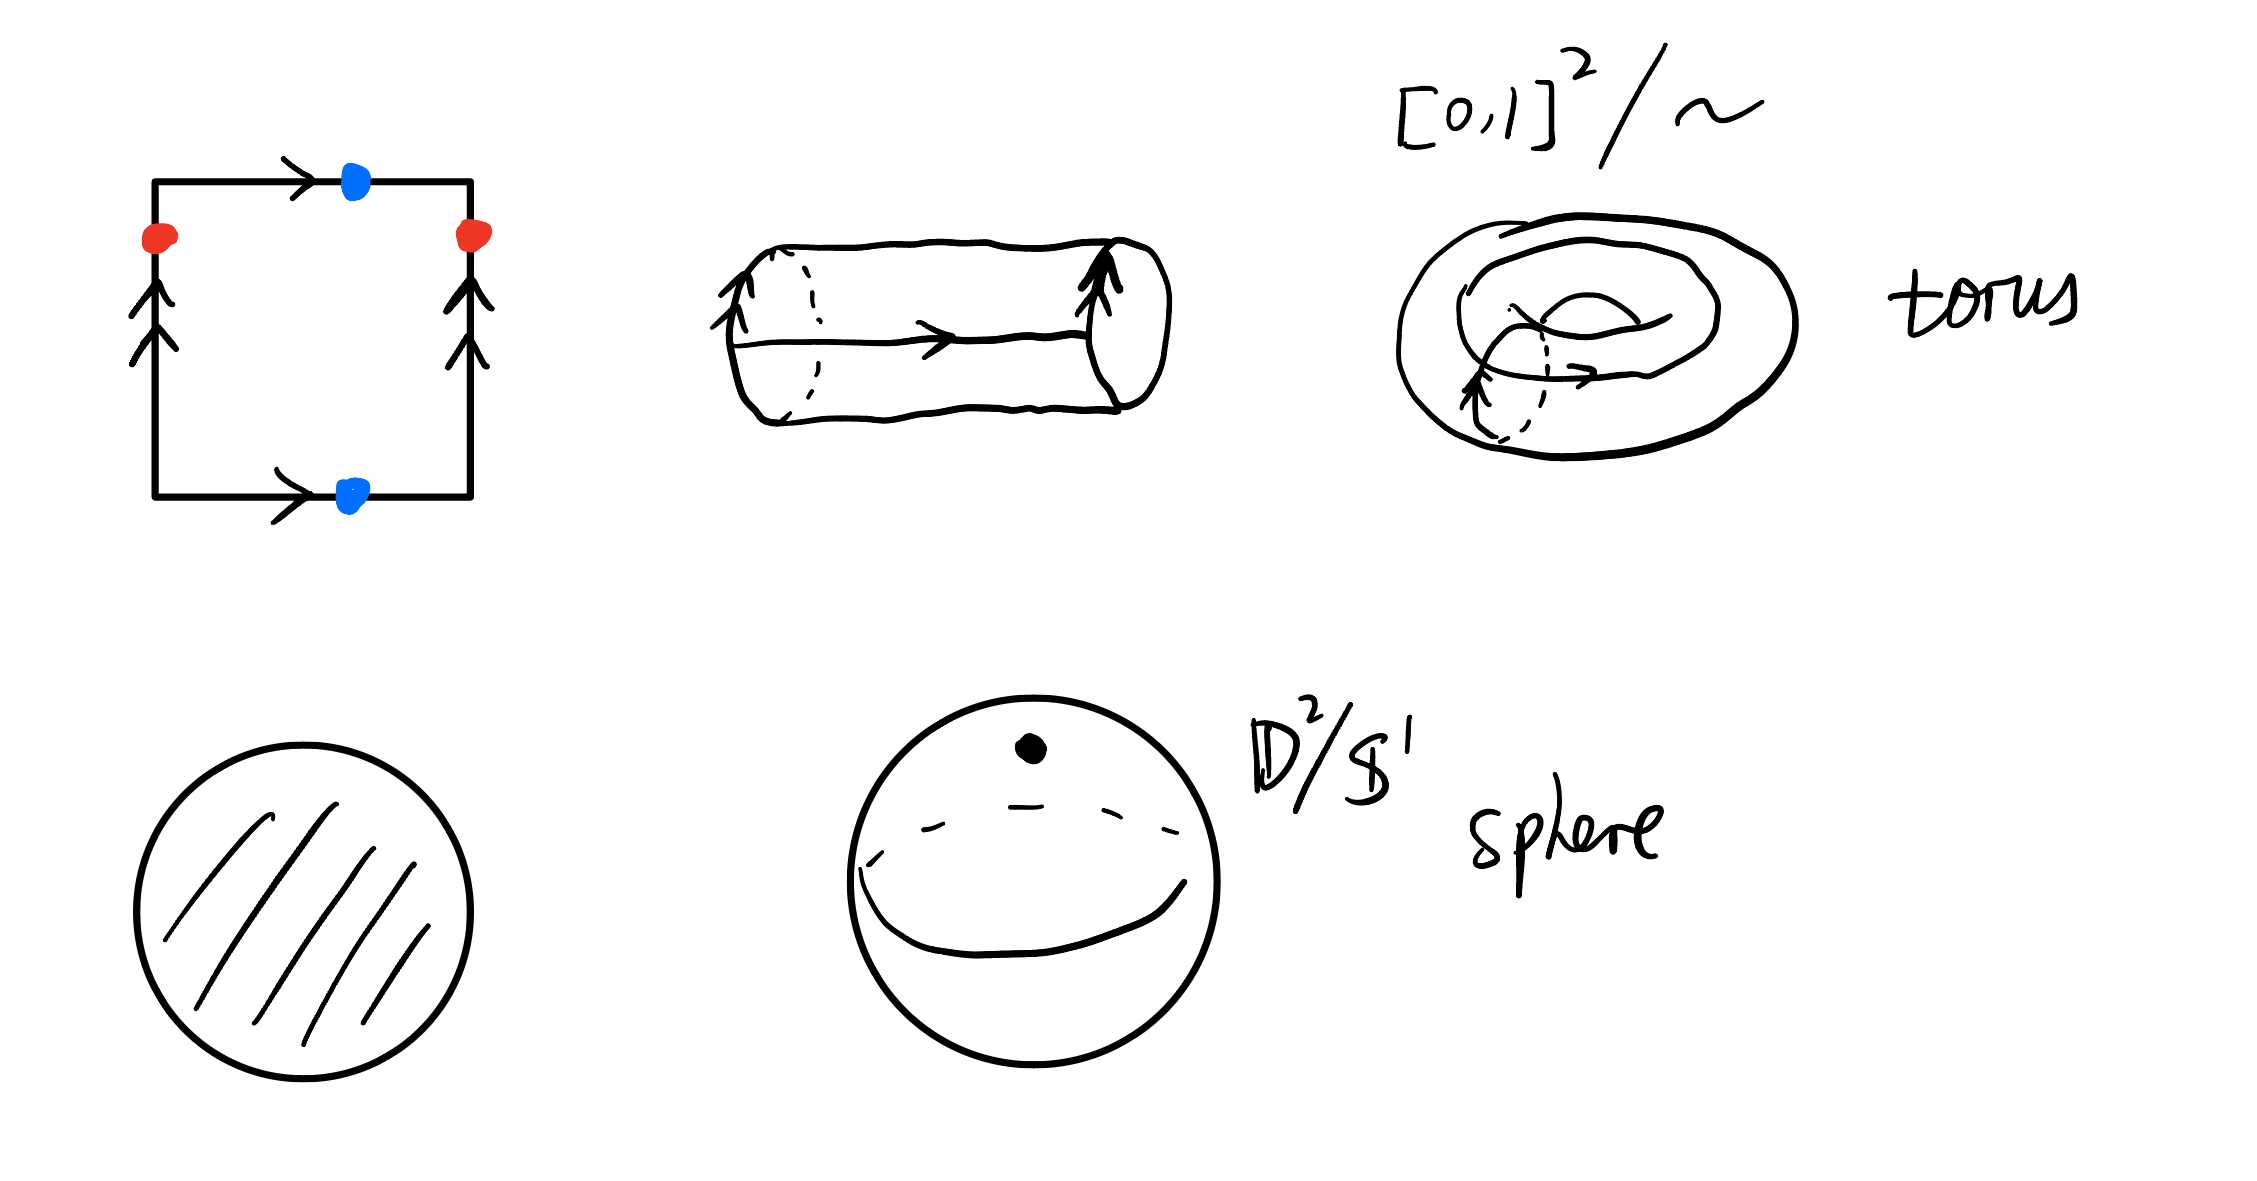
\includegraphics[width=0.8\textwidth]{figures/torus-sphere.png}
\caption{A torus and a sphere, illustrating the concept of quotient spaces.}
\label{fig:torus-sphere}
\end{figure}

\end{example}

How can we get a topology on $X^*$ from the topology on $X$? Recall that the product topology can be characterized via some continuous maps. Maybe we can do something similar here. A very natural map is the quotient map $p:X\to X^*$ sending each point to its equivalence class.

We want the finest topology on $X^*$ that makes $p$ continuous. Thus we declare a subset $U\subseteq X^*$ to be open whenever $p^{-1}(U)$ is open in $X$. This includes every subset that can be open without violating continuity of $p$.




% The product topology on $X=\Pi X_i$ is the weakest topology so that all projections $\pi_i:X\to X_i$ are continuous. Dually, we may consider the strongest topology on $Y$ so that maps $q_i:X_i\to Y$ are continuous. If we just consider one surjective map, we obtain the notion of quotient topology.


\begin{definition}[Quotient topology]
Let $q:X\to Y$ be a surjective map. The \emph{quotient topology} on $Y$ is defined by
\[\tau_q: = \{ V \subseteq Y \mid q^{-1}(V) \text{ is open in } X \}\]
When endowed with the quotient topology, we call $Y$ a \emph{quotient space} of $X$ and $q$ a \emph{quotient map}.
\end{definition}
\begin{proof}[Check: this is indeed a topology]
  $q^{-1}(Y)=X$ and $q^{-1}(\emptyset)=\emptyset$. So $Y,\emptyset\in\tau_q$.

  $q^{-1}(\bigcup_{\alpha} V_\alpha) = \bigcup_{\alpha} q^{-1}(V_\alpha)$, so $\bigcup_{\alpha} V_\alpha \in \tau_q$.

  $q^{-1}(\cap_{i=1}^nV_i) = \cap_{i=1}^n q^{-1}(V_i)$, so $\cap_{i=1}^n V_i \in \tau_q$. 
\end{proof}

\begin{remark}
  The quotient topology is the finest topology on $Y$ making $q$ continuous: if $\tau$ is any topology on $Y$ with $q$ continuous, then $\tau\subseteq \tau_q$.
\end{remark}

\begin{definition}[Quotient space]
  Let $X$ be a topological space. Let $\sim$ be an equivalence relation on $X$ and let $X^*:=X/\sim$ be the set of equivalence classes. The \emph{quotient space} of $X$ by $\sim$ is the set $X^*$ endowed with the quotient topology via the natural projection map $p:X\to X^*$ sending each point to its equivalence class.
\end{definition}

% \begin{remark}
%   Note that we start with $q:X\to X^*$ and then turn to a general surjective map $q:X\to Y$. You should think of $Y$ as $X^*$. Indeed, any surjective map $q:X\to Y$ induces an equivalence relation $\sim$ on $X$ defined by $x\sim x'$ iff $q(x)=q(x')$. Then, $Y$ is in bijection with $X^*=X/\sim$ via the map sending each equivalence class to its image under $q$. So we can identify $Y$ with $X^*$.
%   \begin{center}
%   \begin{tikzcd}[column sep=large]
%   X \arrow[drr, two heads, "q"'] \arrow[rr, two heads, "p"] && X/{\sim} \arrow[d,"\varphi","\cong"'] \\
%   && Y
%   \end{tikzcd}
%   \end{center}

%   More explicitly, let $p:X\to X^*$ be the natural projection. Then we have the quotient topology on $X^*$: 
%   \[\tau_p=\{V\subseteq X^*: p^{-1}(V)=\{x|[x]\in V\} \text{ is open in } X\}.\]

  

% \end{remark}

\begin{example}[A 3–point quotient of $\R$]
Let $p:\R\to Y=\{-1,0,1\}$ be
\[
p(x)=
\begin{cases}
-1,&x<0,\\
0,&x=0,\\
1,&x>0.
\end{cases}
\]
Endow $Y$ with the quotient topology via $p$. A subset $V\subseteq Y$ is open iff $p^{-1}(V)$ is open in $\R$.

\begin{itemize}
  \item $p^{-1}(\{-1\})=(-\infty,0)$ and $p^{-1}(\{1\})=(0,\infty)$ are open $\Rightarrow \{-1\},\{1\}$ are open.
  \item $p^{-1}(\{0\})=\{0\}$ is not open $\Rightarrow \{0\}$ not open.
  \item $p^{-1}(\{-1,1\})=\R\setminus\{0\}=(-\infty,0)\cup(0,\infty)$ is open $\Rightarrow \{-1,1\}$ open.
  \item $p^{-1}(\{-1,0\})=(-\infty,0]$ and $p^{-1}(\{0,1\})=[0,\infty)$ are not open.
\end{itemize}

Thus
\[
\tau_Y=\{\varnothing,\{-1\},\{1\},\{-1,1\},\{-1,0,1\}\}.
\]
\end{example}

\begin{figure}[htbp!]
  \centering
  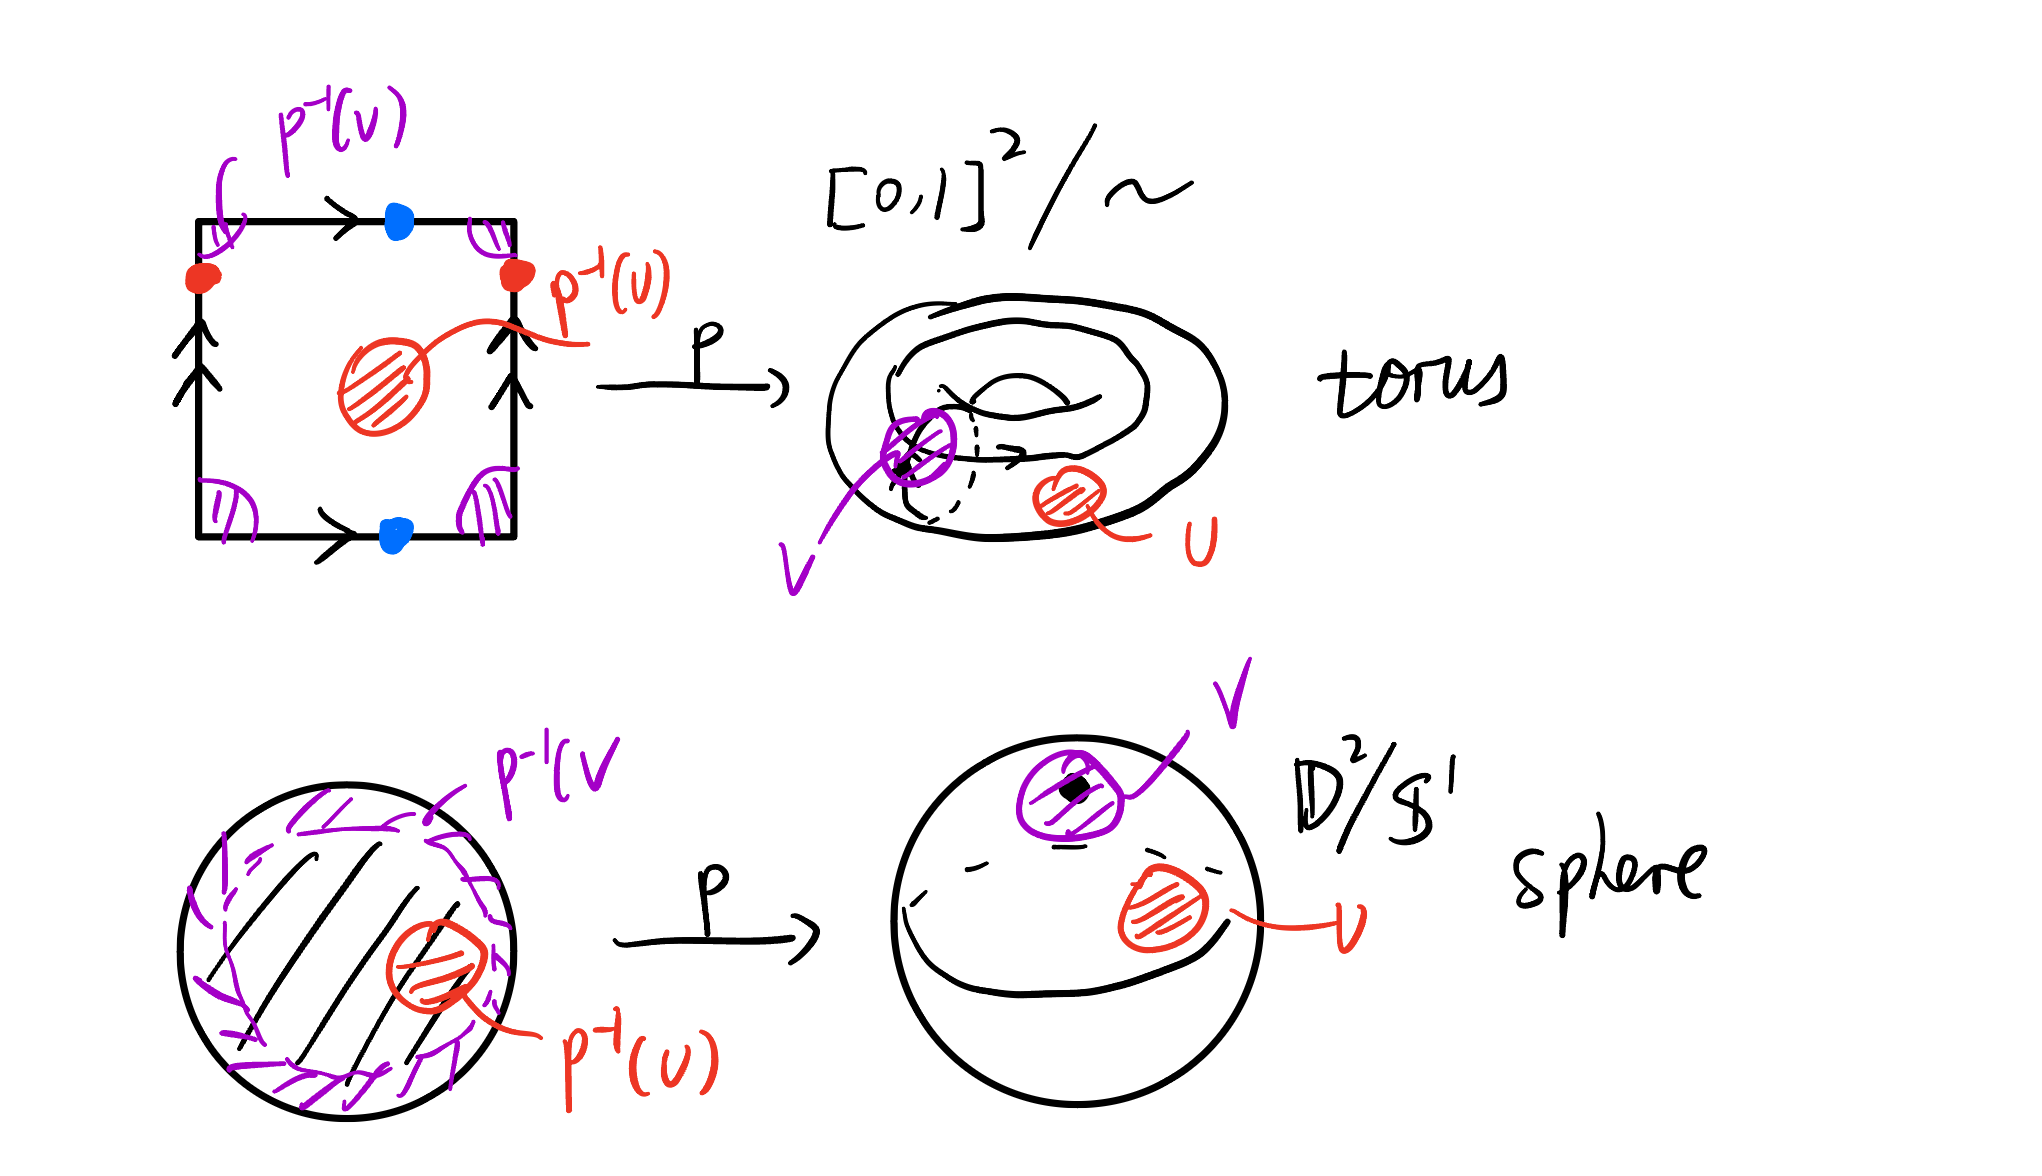
\includegraphics[width=0.8\textwidth]{figures/torus-sphere-subspace.png}
  \caption{A torus and a sphere, illustrating the concept of quotient spaces.}
  \label{fig:torus-sphere-subspace}
  \end{figure}

\begin{example}[Torus and Sphere]
  Consider the maps shown in the image (Figure \ref{fig:torus-sphere-subspace}). We then can endow the torus and the sphere (viewed as subsets of $\R^3$) with the quotient topologies via these maps. Of course, there is the question whether these quotient topologies coincide with the subspace topologies from $\R^3$. We will answer this question later.
\end{example}



\newpage

Now let $q:X\to Y$ be surjective. What if we have another topology $\tau$ on $Y$?

\begin{definition}
  For two topological spaces $X,Y$ and a surjective map $q:X\to Y$, we say $q$ is a \emph{quotient map} if 

  \[\text{a subset $U \subseteq Y$ is open in $Y$ iff $q^{-1}(U)$ is open in $X$.}\]
\end{definition}

In other words, $q$ is a quotient map if the topology on $Y$ coincides with the quotient topology via $q$. 

Whenever we have a quotient map $q:X\to Y$, we can identify $Y$ with the quotient space $X^*$ of $X$ by the equivalence relation induced by $q$. More precisely, we have the following proposition.

\begin{proposition}
  Let $q:X\to Y$ be a quotient map. Define $\sim$ on $X$ by $x\sim x'$ iff $q(x)=q(x')$ and let $X^*:=X/\sim=\{q^{-1}(y): y \in Y\}$ endowed with the quotient topology. Then, $q$ induces a homeomorphism $\varphi:X^*\to Y$ such that the following diagram commutes:
  \begin{center}
  \begin{tikzcd}[column sep=large]
  X \arrow[drr, two heads, "q"'] \arrow[rr, two heads, "p"] && X^{*} \arrow[d,"\varphi"] \\
  && Y
  \end{tikzcd}
  \end{center}
\end{proposition}
\begin{proof}
  We first define $\varphi:X^*\to Y$ by $\varphi(q^{-1}(y))=y$. This is well-defined since $q^{-1}(y)=q^{-1}(y')$ implies $y=y'$. It is easy to see that $\varphi$ is bijective and the diagram commutes.

  Next, we show that $\varphi$ is continuous. For any open set $U\subseteq Y$, we have that
  \[p^{-1}(\varphi^{-1}(U))=q^{-1}(U)\]
is open since $q$ is continuous. By the definition of the quotient topology, $\varphi^{-1}(U)$ is open in $X^*$ and hence $\varphi$ is continuous.

Finally, we show that $\varphi^{-1}$ is continuous. For any open set $V\subseteq X^*$, we have that
\[q^{-1}(\varphi(V))=p^{-1}(V)\]
is open since $p$ is continuous. By the definition of the quotient map, $\varphi(V)$ is open in $Y$ and hence $\varphi^{-1}$ is continuous.
\end{proof}


Here is some simple criterion for quotient maps. A map is said to be \emph{open} if the image of every open set is open. Similarly, a map is said to be \emph{closed} if the image of every closed set is closed.

\begin{theorem}
  Let $q:X\to Y$ be a surjective continuous map. If $q$ is open or closed, then $q$ is a quotient map.
\end{theorem}
\begin{proof}
  We only need to show the ``only if'' direction. Suppose $q$ is open. Let $U\subseteq Y$ be such that $q^{-1}(U)$ (we used surjection here) is open in $X$. Then, $U=q(q^{-1}(U))$ is open in $Y$ since $q$ is open.   
  The case when $q$ is closed is similar.
\end{proof}



\begin{example}[A quotient map that is neither open nor closed]
  Let $A=[0,1)\subset\R$. Identify all points of $A$ with one another and leave every other point distinct: define $x\sim y$ if $x=y$ or both $x,y\in A$. Give $Y=\R/{\sim}$ the quotient topology and let $q:\R\to Y$ be the natural projection. Then $q$ is a quotient map.

  Write $*$ for the point corresponding to $A$. Since
  \[
    q^{-1}(\{*\})=[0,1)
  \]
  is neither open nor closed in $\R$, the singleton $\{*\}$ is neither open nor closed in $Y$.
  But $q((0,1))=\{*\}$ although $(0,1)$ is open, and $q(\{0\})=\{*\}$ although $\{0\}$ is closed. Thus $q$ is neither an open map nor a closed map, so the converse of the preceding theorem fails.
\end{example}

\begin{example}
  Consider the subspace
  \[
  X=\{(x,y)\in\R^2: xy=1\}\ \cup\ \{(0,0)\}\subset\R^2,
  \qquad
  q:X\longrightarrow \R,\; q(x,y)=x.
  \]
  The map \(q\) is surjective: for \(x\neq 0\) choose \(y=1/x\), and \(q(0,0)=0\).
  It is continuous as the restriction of the projection \(\pi_1:\R^2\to\R\).

  However \(q\) is not a quotient map.
  Indeed \(\{(0,0)\}=B_\varepsilon(0,0)\cap X\) for small \(\varepsilon>0\), so \(\{(0,0)\}\) is open in \(X\).
  Thus
  \[
  q^{-1}(\{0\})=\{(0,0)\}\ \text{ is open in } X,
  \]
  but \(\{0\}\) is not open in \(\R\). Thus \(q\) is continuous and surjective, but not a quotient map.
\end{example}

\begin{example}
  Let $X=[0,2\pi]$ with the usual topology from $\R$. Let $Y=S^1=\{(x,y)\in\R^2:x^2+y^2=1\}$ with the subspace topology from $\R^2$. Define
  \[
  p:X\to Y,\quad p(t)=(\cos t,\sin t).
  \]
  Then, $p$ is surjective and continuous. $p$ is not open unfortunately: $[0,a)$ will not be mapped to an open set. But $p$ is closed. Later when we have more tools, this can be proved easily. But now, let's use techniques we have to prove it.

  \begin{proof}[Proof that $p$ is closed]
  Let $F\subset[0,2\pi]$ be closed. We show $p(F)$ is closed in $S^{1}$.
  Since $S^{1}\subset\R^{2}$ is a metric space, it suffices to use sequences.

  Take any sequence $(y_n)\subset p(F)$ with $y_n\to y\in S^{1}$. For each $n$ choose
  $t_n\in F$ such that $p(t_n)=y_n$. The sequence $(t_n)$ lies in the bounded interval
  $[0,2\pi]$, so by Bolzano–Weierstrass it has a convergent subsequence
  $t_{n_k}\to t\in[0,2\pi]$. Because $F$ is closed and each $t_{n_k}\in F$, we have $t\in F$.
  By continuity of $p$,
  \[
  p(t_{n_k}) \longrightarrow p(t).
  \]
  But $p(t_{n_k})=y_{n_k}\to y$, hence $y=p(t)\in p(F)$. Thus every limit of a convergent
  sequence in $p(F)$ lies in $p(F)$; so $p(F)$ is closed in $S^{1}$.

  Therefore $p$ sends closed subsets of $[0,2\pi]$ to closed subsets of $S^{1}$, i.e.\ $p$ is a
  closed map. Since $p$ is surjective and continuous, it is a quotient map.
  \end{proof}

  In this way, we can identify $S^1$ with the quotient space obtained by attaching end points of an interval $[0,2\pi]/(0\sim 2\pi)$.
\end{example}

\begin{remark}
  The gluing maps in the interval, torus, and sphere examples above are quotient maps when the targets are endowed with subspace topologies. In fact, these maps are closed, which we can prove later when we learn about compactness. Right now, we can just use the sequence argument as in the previous example.
\end{remark}



\subsubsection{Universal properties: products and quotients}

Both constructions can be described by how continuous maps factor through them. For a product, we specify a map \emph{into} the product by its coordinates. For a quotient, we obtain a map \emph{out of} the quotient from a map that is constant on each fiber. In each case, the resulting map is unique.

Here \emph{universal} means that the property holds for every topological space $Z$ and every choice of maps satisfying the stated conditions.

\begin{theorem}[Universal property of the product]
\label{theorem: product universal property}
Let $\{X_i\}_{i\in I}$ be a family of topological spaces, and let $P=\prod_{i\in I}X_i$ have the product topology, with coordinate projections $\pi_i:P\to X_i$. Let $Z$ be any topological space and let $g_i:Z\to X_i$ be a function for each $i\in I$. Then there is a unique function $g:Z\to P$ such that
\[
  \pi_i\circ g=g_i\qquad\text{for every }i\in I.
\]
It is defined by $g(z)=(g_i(z))_{i\in I}$. Moreover, $g$ is continuous if and only if $g_i$ is continuous for every $i\in I$.
\end{theorem}

The following diagram commutes for every $i\in I$:
\begin{center}
\begin{tikzcd}[column sep=3.2em,row sep=3.2em]
Z \arrow[r,dashed,"g"] \arrow[dr,"g_i"'] & P \arrow[d,"\pi_i"] \\
& X_i
\end{tikzcd}
\end{center}
\begin{proof}
The formula $g(z)=(g_i(z))_{i\in I}$ defines a function $g:Z\to P$ with $\pi_i\circ g=g_i$ for every $i\in I$. If $h:Z\to P$ also satisfies these identities, then $h(z)$ and $g(z)$ have the same coordinates for every $z\in Z$. Hence $h=g$.

If $g$ is continuous, then each $g_i=\pi_i\circ g$ is continuous, since the projections are continuous. Conversely, if every $g_i$ is continuous, then $g$ is continuous by Theorem~\ref{theorem: product continuous}.
\end{proof}

\begin{theorem}[Universal property of a quotient map]
Let $q:X\to Y$ be a quotient map and let $Z$ be a topological space. Let $g:X\to Z$ be such that $g$ is constant on each fiber $q^{-1}(\{y\})$. Then there is a unique function $f:Y\to Z$ such that $f\circ q=g$, defined by $f(q(x))=g(x)$. Moreover,
\begin{enumerate}
  \item $f$ is continuous iff $g$ is continuous.
  \item $f$ is a quotient map iff $g$ is a quotient map.
\end{enumerate} 
\end{theorem}

\begin{center}
\begin{tikzcd}[column sep=3.2em,row sep=3.2em]
X \arrow[d,"q"'] \arrow[dr,"g"] & \\
Y \arrow[r,dashed,"f"'] & Z
\end{tikzcd}
\end{center}

% \begin{theorem}
% Let $q:X\to Y$ be a quotient map and let $Z$ be a topological space. Let $g:X\to Z$ be \emph{constant on each }  $q^{-1}(\{y\})$. This induces a function $f:Y\to Z$ such that $f\circ q=g$. Then  $f$ is continuous iff $g$ is continuous. 
% \end{theorem}

\begin{proof}
The formula $f(q(x))=g(x)$ is well-defined because $g$ is constant on each fiber of $q$. Since $q$ is surjective, this formula defines $f$ on all of $Y$ and determines it uniquely.

(1) $(\Rightarrow)$ Composition of continuous maps is continuous.

$(\Leftarrow)$ Suppose $g$ is continuous. Let $V\subseteq Z$ be open. Then
\[
(f\circ q)^{-1}(V)=q^{-1}\bigl(f^{-1}(V)\bigr)
\]
is open in $X$. Since $q$ is a quotient map, $f^{-1}(V)$ is open in $Y$; hence $f$ is continuous.


(2) Since $q$ is surjective, $f$ is surjective if and only if $g$ is; their continuity is equivalent by (1). It remains to check the condition on open sets.

$(\Leftarrow)$ Suppose $g$ is a quotient map. Let $U\subseteq Z$ be such that $f^{-1}(U)$ is open in $Y$. Then
\[q^{-1}(f^{-1}(U))=(f\circ q)^{-1}(U)=g^{-1}(U)\]
is open in $X$. Since $g$ is a quotient map, $U$ is open in $Z$. Hence $f$ is a quotient map.

$(\Rightarrow)$ Suppose $f$ is a quotient map. Let $U\subseteq Z$ be such that $g^{-1}(U)$ is open in $X$. Then
\[q^{-1}(f^{-1}(U))=(f\circ q)^{-1}(U)=g^{-1}(U)\]
is open in $X$. Since $q$ is a quotient map, $f^{-1}(U)$ is open in $Y$. Since $f$ is a quotient map, $U$ is open in $Z$. Hence $g$ is a quotient map. The same proof shows that the composition of two quotient maps is a quotient map.
\end{proof}

% As a consequence, we prove the other direction of a quotient map proposition above.

% \begin{corollary}
%   Let $q:X\to Y$ be a surjective continuous map and let $X^*=\{q^{-1}(\{y\}): y \in Y\}$ endowed with the quotient topology. 
%   Then, the map $q$ induces a bijective continuous map $\varphi:X^*\to Y$, which is a homeomorphism iff $q$ is a quotient map.
% \end{corollary}

% \begin{proof}


%   We already proved the if part.

%   For the only if part, 
%   It is easy to see that $\varphi$ is bijective. If $\varphi$ is a homeomorphism, then $\varphi^{-1}$ is continuous. By the theorem above, $p\circ \varphi^{-1}$ is continuous iff $\varphi^{-1}$ is continuous. But $p\circ \varphi^{-1}=q$. So $q$ is a quotient map.
% \end{proof}



% \begin{example}[Circle as a quotient]
% Identify $0\sim 1$ in $[0,1]$; let $p:[0,1]\to [0,1]/(0\sim 1)$. Define
% \[
% g:[0,1]\to S^{1},\qquad g(t)=(\cos 2\pi t,\sin 2\pi t).
% \]
% Then $g(0)=g(1)$, so $g$ is constant on fibers of $p$. By the theorem there is a unique continuous $f:[0,1]/(0\sim 1)\to S^{1}$ with $f\circ p=g$, giving a homeomorphism.
% \end{example}

% \begin{example}[Torus from a square]
% Let $X=[0,1]^2$ and identify opposite edges: $(0,y)\sim(1,y)$ and $(x,0)\sim(x,1)$. The quotient $T=X/{\sim}$ is a torus. The map
% \[
% g:[0,1]^2\to S^{1}\times S^{1},\qquad g(x,y)=\big(e^{2\pi i x},e^{2\pi i y}\big)
% \]
% is continuous and constant on each equivalence class, hence descends to a continuous bijection $f:T\to S^{1}\times S^{1}$; one checks $f$ is a homeomorphism.
% \end{example}


% The quotient topology usually arises in the context of identifying points in a space, such as when we take a space and "collapse" certain subsets to points. Essentially, since we are only considering surjective maps, we can think of each point in $Y$ as an equivalence class of points in $X$.



% Let $X$ be a topological space and let $\sim$ be an equivalence relation on $X$. We would like to introduce a topology on the set of equivalence classes 
% $$X^*=X/\sim=\{[x] \mid x \in X\}.$$

% \begin{theorem}
%   Define the map $q:X \to X^*$ sending $x \mapsto [x]$. Then, its quotient topology is identified as follows: a set $U \subseteq X^*$ is open if and only if $q^{-1}(U)=\bigcup_{[x] \in U} [x]$ is open in $X$, where $[x]$ denotes the equivalence class of $x$.
% \end{theorem}

% \begin{example}
% Identify the endpoints of $[0,1]$ to form a circle: let $q:[0,1]\to S^1$ send $t\mapsto (\cos 2\pi t, \sin 2\pi t)$. The resulting topology on $S^1$ is the quotient of the interval by $0\sim1$.
% \end{example}

% \begin{example}[Cylinder from a square]
% Let $X=[0,1]\times[0,1]$ and define an equivalence relation $\sim$ by
% \[
% (x,0)\sim (x,1)\quad\text{for all }x\in[0,1],
% \]
% where only the bottom and top edges are identified (orientation preserved). Then the quotient $X^*=X/{\sim}$ is homeomorphic to $\mathbb{S}^1\times[0,1]$, the (closed) cylinder. A convenient homeomorphism is
% \[
% X^*\to\mathbb{S}^1\times[0,1],\qquad [x,y]\mapsto\big(e^{2\pi i x},\,y\big),
% \]
% with inverse given by any continuous choice of argument on $\mathbb{S}^1$ composed with the projection onto the first coordinate.
% \end{example}

% \begin{example}[Torus from a square]
% Let $X=[0,1]\times[0,1]$ and define an equivalence relation $\sim$ by
% \[
% (x,0)\sim (x,1)\quad\text{for all }x\in[0,1],\qquad
% (0,y)\sim (1,y)\quad\text{for all }y\in[0,1],
% \]
% where the identifications preserve the orientations of the edges. 

% You should verify that $X^*=X/{\sim}$ is homeomorphic to the product space $\mathbb{S}^1\times \mathbb{S}^1$, which is the torus.
% \end{example}

% \begin{example}[Collapsing the boundary of a disk yields a sphere]
% Let \(D^2=\{x\in \mathbb{R}^2:\|x\|\le 1\}\) and define an equivalence relation on \(D^2\) by
% \[
% x\sim y\iff x=y \text{ or} x,y\in\partial D^2.
% \]
% Write \(D^2/\partial D^2\) for the quotient space obtained by collapsing the entire boundary \(\partial D^2\) to a single point. You can verify \(D^2/\partial D^2\) is homeomorphic to the 2‑sphere \(S^2\).
% \end{example}

\newpage

\subsection{Homotopy}

\begin{example}
  $\R$ and $\R^2$ are not homeomorphic. How about $\R^2$ vs $\R^3$?
\end{example}

We would like to answer this question to some extent. In the process of answering this question, we will introduce a very important concept in topology, called homotopy.


\begin{definition}
    Let $f$ and $g$ be continuous maps from a topological space $X$ to a topological space $Y$.  We say that $f$ and $g$ are \emph{homotopic} if there exists a continuous map $H\colon X\times [0,1]\to Y$ such that $H(x,0)=f(x)$ and $H(x,1)=g(x)$ for all $x\in X$. $H$ is called a \emph{homotopy} between $f$ and $g$. We write $f\simeq g$ to indicate that $f$ and $g$ are homotopic.
\end{definition}

\begin{example}
  Any continuous map $f\colon X\to Y$ is homotopic to itself via the constant homotopy $H(x,t)=f(x)$.
\end{example}

\begin{example}
    In $\R^n$ the identity map $f(x)=x$ is homotopic to the constant map $g(x)=0$ via the \emph{straight--line homotopy}
    \[
        H(x,t)=(1-t)x.
    \]
\end{example}

\begin{example}
    More generally, if $Y$ is a convex subset of some $\R^n$ and $f,g\colon X\to Y$ are continuous, then
    \[
        H(x,t)= (1-t)f(x)+t g(x)
    \]
    defines a homotopy $f\simeq g$. Thus any two maps into a convex (in particular, contractible) space are homotopic. The target matters: regarded as maps $S^1\to D^2$ the identity and any constant map are homotopic, but as maps $S^1\to S^1$ they need not be. This is in fact quite nontrivial and we will return to it later.
\end{example}

\begin{proposition}
    Homotopy is an equivalence relation on $C(X,Y)$, the set of continuous maps $X\to Y$.
\end{proposition}

\begin{proof}
    Reflexivity: $f\simeq f$ via the constant homotopy $H(x,t)=f(x)$. 
    
    Symmetry: if $H$ is a homotopy $f\simeq g$, then $H'(x,t)=H(x,1-t)$ is a homotopy $g\simeq f$. 
    
    Transitivity: if $H_1$ is a homotopy $f\simeq g$ and $H_2$ a homotopy $g\simeq h$, define
    \[
        H(x,t)=
        \begin{cases}
            H_1(x,2t) & 0\le t\le \frac12,\\[2pt]
            H_2(x,2t-1) & \frac12\le t\le 1.
        \end{cases}
    \]
    Continuity follows from the pasting lemma (here we used the fact that the product of two closed sets is closed) because the two pieces agree at $t=\frac12$. Then $H$ is a homotopy $f\simeq h$.

    
\end{proof}

\begin{proposition}[Composites of homotopic maps are homotopic]
If $f_1,g_1\colon X\to Y$ and $f_2,g_2\colon Y\to Z$ with $f_1\simeq g_1$ and $f_2\simeq g_2$, then $f_2\circ f_1\simeq g_2\circ g_1$.
\end{proposition}

\begin{proof}
Let $H_1\colon X\times I\to Y$ be a homotopy $f_1\simeq g_1$ and $H_2\colon Y\times I\to Z$ a homotopy $f_2\simeq g_2$. Then $f_2\circ H_1$ is a homotopy $f_2\circ f_1\simeq f_2\circ g_1$. Define $H(x,t)=H_2(g_1(x),t)$; this is continuous as a composite and gives a homotopy $f_2\circ g_1\simeq g_2\circ g_1$. Transitivity yields $f_2\circ f_1\simeq g_2\circ g_1$.
\end{proof}

With the notion of homotopy between functions, we can define homotopy equivalence between spaces.

\begin{definition}
Two spaces $X$ and $Y$ are \emph{homotopy equivalent} if there exist continuous maps $f\colon X\to Y$ and $g\colon Y\to X$ such that $g\circ f\simeq id_X$ and $f\circ g\simeq id_Y$. In this case $f$ and $g$ are homotopy inverses and we write $X\simeq Y$.
\end{definition}

\begin{remark}
Homotopy equivalence is an equivalence relation on spaces. Any homeomorphism is a homotopy equivalence (take $g=f^{-1}$). The converse fails; see the example below.
\end{remark}

One special case of homotopy equivalence is when one of the spaces is a point.

\begin{definition}
A space $X$ is \emph{contractible} if the identity map $id_X$ is homotopic to a constant map $c_{x_0}\colon X\to X$ sending every point to $x_0$. Equivalently, there exists $H\colon X\times I\to X$ with $H(x,0)=x$ and $H(x,1)=x_0$ for all $x$. 
\end{definition}

\begin{theorem}
A space $X$ is contractible iff it is homotopy equivalent to a one--point space.
\end{theorem}

\begin{proof}
If $X$ is contractible pick $x_0\in X$ and set $Y=\{x_0\}$. Let $j\colon Y\hookrightarrow X$ be inclusion and $c\colon X\to Y$ the constant map. Then $c\circ j=id_Y$ and $j\circ c=c\simeq id_X$, so $X\simeq Y$.

Conversely, suppose $f\colon X\to Y$ and $g\colon Y\to X$ exhibit a homotopy equivalence where $Y$ is a point. Then $g\circ f$ is constant and $g\circ f\simeq id_X$, giving a homotopy from $\id_X$ to a constant map, so $X$ is contractible.
\end{proof}

\begin{example}
Every convex subset of $\R^n$ (in particular $\R^n$ and any disk $D^n$) is contractible via the straight--line homotopy $H(x,t)=(1-t)x+t x_0$.
\end{example}





\begin{example}
  $\R^n$ is contractible but $\R^n$ is not homeomorphic to a point.
\end{example}

\begin{example}
  $S^1$ is not contractible. We will prove this later.
\end{example}

The contractible case is the trivial case of homotopy equivalence. More generally, we can often find a smaller subspace which is homotopy equivalent to the whole space. This is made precise by the following definitions.


\begin{definition}
Let $A\subseteq X$. A map $r\colon X\to A$ is a \emph{retraction} if $r(a)=a$ for all $a\in A$ (equivalently $r\circ i=\id_A$ where $i\colon A\hookrightarrow X$ is inclusion).
\end{definition}

\begin{definition}
A subspace $A\subseteq X$ is a \emph{deformation retract} of $X$ if there is a retraction $r\colon X\to A$ such that there is a homotopy $H\colon X\times I\to X$ with $H(x,0)=x$, $H(x,1)=r(x)$, and $H(a,t)=a$ for all $a\in A$, $t\in I$. We call $H$ a \emph{deformation retraction}.
\end{definition}

\begin{proposition}
If $A$ is a deformation retract of $X$ then $A\simeq X$. Thus a deformation retract gives a special homotopy equivalence (with inverse given by the retraction).
\end{proposition}

\begin{proof}
Let $r\colon X\to A$ be a retraction and $i\colon A\hookrightarrow X$ inclusion with $i\circ r\simeq \id_X$. Then $r\circ i=\id_A$, so $i$ and $r$ are homotopy inverses.
\end{proof}

\begin{example}
  \begin{enumerate}
    \item The circle $S^1$ is a deformation retract of any annulus $A=\{x\in \R^2 : 1\le \lVert x\rVert \le R\}$ with the retraction $r(x)=x/\lVert x\rVert$ and the homotopy $H(x,t)=(1-t)x+t r(x)$.
    \item $\R^n\setminus\{0\}$ deformation retracts onto $S^{n-1}$: the retraction is $r(x)=x/\lVert x\rVert$ and the homotopy is $H(x,t)=(1-t)x+t r(x)$.
  \end{enumerate}
\end{example}

\begin{example}
  Not every retraction is a deformation retraction. In fact, for any $X$ and $x_0\in X$, the constant map $c_{x_0}\colon X\to \{x_0\}$ is a retraction if $\{x_0\}$ is a retract of $X$, but it is a deformation retraction only if $X$ is contractible.
\end{example}

\begin{theorem}
  There is no retraction $D^2\to S^1$.
\end{theorem}

This can be proved using algebraic topology (fundamental group) or using homology. We will give a proof without these later.

Now we are ready to answer the question whether $\R^2$ and $\R^3$ are homeomorphic. 

\begin{theorem}
$\R^2$ is not homeomorphic to $\R^3$.
\end{theorem}

\begin{proof}
Suppose on the contrary there is a homeomorphism $f\colon \R^2\to \R^3$. Then $f$ restricts to a homeomorphism $\R^2\setminus\{0\}\to \R^3\setminus\{f(0)\}$. But $\R^2\setminus\{0\}\simeq S^1$ and $\R^3\setminus\{f(0)\}\simeq S^2$. So $S^1\simeq S^2$. We will show this is not true.

We will use the following lemmas.

\begin{lemma}\label{lem:circle-not-contractible}
  The identity map on $S^1$ is not homotopic to a constant map. (This proves $S^1$ is not contractible.)
\end{lemma}

\begin{lemma}\label{lem:sphere-contractible}
  Every map $S^1\to S^2$ is homotopic to a constant map.
\end{lemma}

Now suppose $S^1\simeq S^2$ via maps $f\colon S^1\to S^2$ and $g\colon S^2\to S^1$. Then, we know that $f$ is homotopic to a constant map $c:S^1\to S^2$. So $g\circ f:S^1\to S^1$ is homotopic to $g\circ c$, which is a constant map. But $g\circ f\simeq \id_{S^1}$, which contradicts the first lemma.



\end{proof}

The proof of the first lemma is as follows.

\begin{proof}[Proof of Lemma \ref{lem:circle-not-contractible}]
  We need the following lemma.
  \begin{lemma}[Lifting lemma]
  Let $p:\R\to S^{1}$ be $p(t)=e^{it}$. If $f:S^{1}\to S^{1}$ is homotopic to a constant map, than $f$ lifts, i.e., there exists a continuous $\tilde f:S^{1}\to\R$ with $p\circ\tilde f=f$.
  \end{lemma}
  \begin{proof}
We first show that if $g:S^1\to S^1$ lifts and $h:S^1\to S^1$ satisfies $h(x)\neq -g(x)$ for all $x\in S^1$, then $h$ lifts. Indeed, $h(x)/g(x)\in S^1$ (viewed as complex numbers) is never $-1$, so we can write $h(x)/g(x)=e^{i\psi(x)}$ with a unique continuous $\psi(x)\in(-\pi,\pi)$. If $\tilde g$ is a lift of $g$, i.e., $g(x)=e^{i\tilde g(x)}$, then $h(x)=g(x)e^{i\psi(x)}=e^{i(\tilde g(x)+\psi(x))}$, so $\tilde h(x)=\tilde g(x)+\psi(x)$ is a lift of $h$.


Now, let $H:S^{1}\times I\to S^{1}$ be a homotopy from the constant map $c(z)=1$ to $f$. Equip $S^{1}$ with the chord metric $d(u,v)=|u-v|$ (so $d(u,v)=2$ iff $v=-u$). Since $H$ is uniformly continuous on the compact set $S^{1}\times I\subset\R^3$, choose $\delta>0$ so that
  \[
  |t-s|<\delta\ \Longrightarrow\ d\big(H(z,t),H(z,s)\big)<2\quad\text{for all }z\in S^{1}.
  \]
  Pick $0=t_0<t_1<\dots<t_N=1$ with $t_{j+1}-t_j<\delta$.

  The map $H(\,\cdot\,,0)=c_{1}$ lifts to $\tilde H_N:S^{1}\to\R$ by $\tilde H_N(z)\equiv 0$.

  Inductive step. Suppose $H_{j}$ lifts. For any $z$, the points
  $H(z,t_j)\neq H(z,t_{j+1})$ since $d(H(z,t_j),H(z,t_{j+1}))<2$, so $H(z,t_{j+1})$ lifts as well.

  By induction we have that $f=H(\cdot, 1)$ lifts.
  \end{proof}

  Now, suppose $\id_{S^1}$ is homotopic to a constant map. Then, by the lifting lemma, $\id_{S^1}$ lifts to a continuous map $\tilde f:S^1\to \R$ with $p\circ \tilde f=\id_{S^1}$. The lift $\tilde f$ must be injective because $\id_{S^1}$ is injective. This would violate the intermediate value theorem: choose $\alpha\in (\phi(-1),\phi(1))$ (here we assume $\phi(-1)<\phi(1)$). Then both arcs in $S^1$ from -1 to 1 must contain a point $z$ with $\phi(z)=\alpha$, contradicting injectivity. 
\end{proof}

\begin{proof}[Proof of Lemma \ref{lem:sphere-contractible}]
  Let $f:S^1\to S^2$ be continuous. Pick $p\in S^2\setminus f(S^1)$. ($f$ could be surjective but let's ignore this case and it can be fixed using some more arguments).


  Observe that $S^2-\{p\} \cong \mathbb{R}^2$. Let $g:S^2-\{p\} \to \mathbb{R}^2$ be a homeomorphism. Then, $g\circ f:S^1\to \mathbb{R}^2$ is continuous. Since $\mathbb{R}^2$ is convex, $g\circ f$ is homotopic to a constant map via the straight--line homotopy. Composing with $g^{-1}$ gives a homotopy from $f$ to a constant map. More precisely, if $H_1:S^1\times I\to \mathbb{R}^2$ is a homotopy from $g\circ f$ to a constant map, then $H_2=g^{-1}\circ H_1:S^1\times I\to S^2-\{p\}\hookrightarrow S^2$ is a homotopy from $f$ to a constant map.

  
\end{proof}

\newpage

\subsubsection*{Brouwer Fixed Point Theorem}

Now, we introduce some interesting results and prove some special cases using the fact that $S^1$ is not contractible.

\begin{theorem}[No retraction]
There is no retraction $D^n\to S^{n-1}$ for $n\ge 1$.
\end{theorem}
\begin{proof}
  We prove the case when $n=2$. Suppose there is a retraction $r:D^2\to S^1$. Then, we define $H:S^1\times I\to S^1$ as follows:
  \[H(x,t)=r(tx).
  \]
  Then, $H(x,0)=r(0)$ is a constant map and $H(x,1)=r(x)=x$. So $H$ is a homotopy from the identity map on $S^1$ to a constant map. This contradicts Lemma \ref{lem:circle-not-contractible}.
\end{proof}

\begin{proof}
If $r\colon D^n\to S^{n-1}$ were a retraction, compose any map $S^{n-1}\to D^n$ extending $\id_{S^{n-1}}$ with $r$ to obtain a fixed–point–free self map of $D^n$, contradicting Brouwer.
\end{proof}

\begin{corollary}[Brouwer Fixed Point]
For every $n\ge 1$, any continuous map $F\colon D^n\to D^n$ has a fixed point, i.e.\ there exists $x\in D^n$ with $F(x)=x$.
\end{corollary}

\begin{proof}
Assume $F$ has no fixed point. For each $x\in D^n$ draw the ray starting at $F(x)$ through $x$ and let $r(x)$ be the first intersection of that ray with $S^{n-1}=\partial D^n$. This gives a continuous map $r\colon D^n\to S^{n-1}$ which restricts to the identity on $S^{n-1}$, hence a retraction. But $S^{n-1}$ is not a retract (indeed not a deformation retract) of $D^n$ (proved earlier using homotopy ideas). Contradiction.
\end{proof}



\subsubsection*{Homotopy equivalence = embedding + retraction}



If there is one thing that you need to remember, that is homotopy equivalence is basically embedding + retraction.

First of all, we introduce the notion of embeddings.
\begin{definition}[Embedding]
A continuous map $f:X\to Y$ is an \emph{embedding} if it is a homeomorphism onto its image $f(X)$ (with the subspace topology inherited from $Y$). In particular, $f$ is injective.
\end{definition}

\begin{definition}
  Let $X$ and $Y$ be two disjoint topological spaces. Then, the \emph{disjoint union} of $X$ and $Y$ is the topological space
  \[X\sqcup Y
  \]
  whose underlying set is the disjoint union of sets $X$ and $Y$ and whose topology is given by
  \[U\subseteq X\sqcup Y \text{ is open } \iff U\cap X \text{ is open in } X \text{ and } U\cap Y \text{ is open in } Y.
  \]
  Equivalently, the topology is given by
  \[\tau_{X\sqcup Y}=\{U\sqcup V \mid U\in \tau_X, V\in \tau_Y\}.
  \]
\end{definition}

\begin{definition}[Mapping cylinder]
Given a continuous map $f:X\to Y$, the \emph{mapping cylinder} of $f$ is
\[
M_f=(X\times[0,1])\sqcup Y \big/ \sim
\]
where $(x,1)\sim f(x)$ for all $x\in X$.
Write $[x,t]$ for the class of $(x,t)$ and $[y]$ for $y\in Y$. There are canonical embeddings
\[
i_X:X\hookrightarrow M_f,\qquad x\mapsto [x,0], \qquad\text{and}\qquad
i_Y:Y\hookrightarrow M_f,\qquad y\mapsto [y].
\]
There is a deformation retraction $H:M_f\times I\to M_f$ onto $i_Y(Y)$ given by
$H([x,t],s)=[x,(1-s)t+ s]$ and $H([y],s)=[y]$, so $M_f$ deformation retracts onto $Y$.
\end{definition}

\begin{lemma}
  For any continuous map $f:X\to Y$, the map $H:M_f\times I \to M_f$ defined by $H([x,t],s):=[x,(1-s)t+ s]$ and $H([y],s):=[y]$ is a deformation retraction of $M_f$ onto $i_Y(Y)$. 
\end{lemma}

\begin{lemma}
  $f:X\to Y$ is a homotopy equivalence if and only if $i_X(X)$ is a deformation retract of $M_f$.
\end{lemma}

\begin{theorem}[Common deformation–retract envelope]
For topological spaces $X$ and $Y$, the following are equivalent:
\begin{enumerate}
    \item $X$ and $Y$ are homotopy equivalent.
    \item There exists a space $Z$ and embeddings $i_X:X\hookrightarrow Z$, $i_Y:Y\hookrightarrow Z$
                such that $i_X(X)$ and $i_Y(Y)$ are each \emph{deformation retracts} of $Z$
                (possibly via two different homotopies).
\end{enumerate}
\end{theorem}

\begin{proof}
$(2)\Rightarrow(1)$: If $Z$ deformation retracts onto $i_X(X)$ and onto $i_Y(Y)$, then
$Z\simeq X$ and $Z\simeq Y$, hence $X\simeq Y$ by transitivity.

$(1)\Rightarrow(2)$: Suppose $f:X\to Y$ is a homotopy equivalence. Form the mapping cylinder
$M_f$, which admits deformation retractions onto $Y$ and $X$.
\end{proof}





\newpage


\section{Continuity and Convergence}



\subsection{Convergence in Topological Spaces}

We will try to answer the following questions:

\begin{enumerate}
    \item Can we define sequential convergence in general topological spaces?
    \item If so, does this convergence describe the notion of topology?
\end{enumerate}

In metric space setting, we have the notion of convergence of a sequence (in the language of open balls):

\begin{proposition}
    A sequence $(x_n)_{n\in\mathbb{N}}$ in a metric space $X$ converges to a point $x\in X$ if and only if for every $\epsilon>0$, there exists $N\in\mathbb{N}$ such that $x_n\in B_\epsilon(x)$ for all $n\ge N$.
\end{proposition}

This motivates the following definition in general topological spaces:



\begin{definition}
    A sequence $(x_n)_{n\in\mathbb{N}}$ in a topological space $X$ is said to converge to a point $x\in X$ if for every neighbourhood $U$ of $x$, there exists $N\in\mathbb{N}$ such that $x_n\in U$ for all $n\ge N$.
\end{definition}

\begin{problem}
    A sequence $(x_n)$ in a metric space converges in the metric sense if and only if it converges in the topological sense defined above.
\end{problem}
\begin{proof}
    ($\Rightarrow$) Let $(x_n)$ be a sequence in a metric space $(X,d)$ converging to $x\in X$ in the metric sense. For every neighborhood $U$ of $x$, there exists $\epsilon>0$ such that $B_\epsilon(x)\subseteq U$. Then, there exists $N$ such that $d(x_n,x)<\epsilon$ for all $n\ge N$. In particular, $x_n\in B_\epsilon(x)\subset U$ for all $n\ge N$. So we have $x_n\to x$ in the topological sense.

    ($\Leftarrow$) Let $(x_n)$ be a sequence in a metric space $(X,d)$ converging to $x\in X$ in the topological sense. For every $\epsilon>0$, the open ball $B_\epsilon(x)$ is a neighbourhood of $x$, so there exists $N$ such that $x_n\in B_\epsilon(x)$ for all $n\ge N$. This means that $d(x_n,x)<\epsilon$ for all $n\ge N$. Hence, $(x_n)$ converges to $x$ in the metric sense.
\end{proof}



\begin{proposition}
   Let $X$ be a topological space. For $A\subseteq X$ and $x\in X$, if there is a sequence $(a_n)\subseteq A$ with $a_n\to x$, then $x\in\overline{A}$.
\end{proposition}
\begin{proof}
    Let $U$ be any neighbourhood of $x$. Then there exists $N$ such that $a_n\in U$ for all $n\ge N$. In particular, $a_N\in A\cap U$, so $A\cap U\neq \emptyset$. Since $U$ was arbitrary, we have $x\in\overline{A}$.
\end{proof}

We know the converse is true in metric spaces. Is it true in general topological spaces?


% \begin{definition}
%     A topological space $X$ is first countable if every point $x\in X$ has a countable neighbourhood basis.
% \end{definition}

% Under this assumption, we have the following characterization of convergence:
% \begin{theorem}
%     If $X$ is first countable and $E\subset X$, then $x\in\overline{E}$ iff there exists a sequence $(x_n)_{n\in\mathbb{N}}$ in $E$ such that $x_n\to x$.
% \end{theorem}

% \begin{corollary}
%     Let $X$ and $Y$ be first countable topological spaces. Then,
%     \begin{enumerate}
%         \item $U\subset X$ is open iff whenever $x_n\to x\in U$, $x_n$ is eventually in $U$.
%         \item $F\subset X$ is closed iff whenever $(x_n)\subset F$, $x_n\to x$, then $x\in F$.
%         \item $f:X\to Y$ is continuous iff whenever $x_n\to x\in X$, then $f(x_n)\to f(x)\in Y$.
%     \end{enumerate}
% \end{corollary}

% For first countable spaces, the notion of sequential convergence describes the topology.


\begin{example}
Let $X=\R$ be endowed with the 
\emph{countable complement topology}: a set $U\subseteq X$ is open 
iff $X\setminus U$ is countable or $U=\emptyset$. 

\begin{itemize}
  \item Any sequence $(x_n)$ converging to $x$ is eventually equal to $x$.  
  Indeed, we let $B=\{x_n:\,x_n\neq x\}$ and hence $U=X\setminus B$ is an 
  open neighborhood of $x$. Then, there exists $N$ such that $x_n\in U$ for all
  $n\ge N$, i.e., $x_n\notin B$ for all $n\ge N$. This means that 
  $x_n=x$ for all $n\ge N$.
  \item The closed sets are exactly the countable sets and $X$ itself.  
  Hence, if $A\subsetneq X$ is uncountable, then 
  $\overline{A}=X$.
\end{itemize}

Thus $\overline{[0,1]}=\R$, but there is no sequence in $[0,1]$ converging to $2$.
\end{example}

Let's see another example.

\begin{example}
    Let $X=\R^\R$ be endowed with the product topology. We consider 
    $$E=\{f\in \R^\R:f(x)=0\text{ or }1\text{ and }f(x)=0\text{ only finitely often}\}.$$

    Let $\mathbf{0}$ denote the all 0 function in $X$. Note that any basis element of the product topology containing $\mathbf{0}$ is of the form
    $$V=\{g\in \R^\R:g(x_i)\in U_i\text{ for }i=1,\ldots,n\}$$
    for some $x_1,\ldots,x_n\in\R$ and open sets $U_i\ni\R$ containing $0$. We now define $g:\R\to \R$ as follows: $g(x_i)=0$ for $i=1,\ldots,n$ and $g(x)=0$ otherwise. Then, $g\in E\cap V$ and hence $E\cap V\neq\emptyset$. Hence, $\mathbf{0}\in\overline{E}$.
    
    Now let $(f_n)$ be a sequence in $E$ such that each $f_n$ is 0 on a finite set $A_n\subset \R$. If $(f_n)$ converges to $f$, then $f$ can be zero at most on the countable set $\bigcup_{n} A_n$. Suppose otherwise $f(x)=0$ for some $x\notin \bigcup_n A_n$. Pick the basic open neighbourhood
    $$U=\{g\in \R^\R:g(x)\in (-1,1)\}.$$
    Then, there exists $N$ such that $f_n\in U$ for all $n\ge N$. In particular, $f_n(x)\in (-1,1)$ for all $n\ge N$. This implies that $f_n(x)=0$ for all $n\ge N$, contradicting the choice of $x$.
    
    Hence, there is no sequence in $E$ converging to $\mathbf{0}$.
\end{example}

In metric spaces, the limit of a convergent sequence is unique. Is this true in general topological spaces?

\begin{example}
    Let $X$ be endowed with the trivial topology $\tau=\{\emptyset,X\}$. Then the constant sequence $(x_n)$ with $x_n=a\in X$ for all $n\in\mathbb{N}$ converges to every point in $X$. 
\end{example}

\begin{example}
    Let $X=\{a,b\}$ with the topology $\tau=\{\emptyset,\{a\},X\}$. Then the constant sequence $(x_n)$ with $x_n=a$ for all $n\in\mathbb{N}$ converges to $a$ and $b$. 
\end{example}

In general, the limit of a convergent sequence may not be unique. We will need to give some additional conditions on the topology to ensure uniqueness of limits.

Finally, let's talk about continuity.

\begin{proposition}
    Let $f:X\to Y$ be continuous at $x$. Then, whenever $x_n\to x$ in $X$, we have $f(x_n)\to f(x)$ in $Y$.
\end{proposition}
\begin{proof}
    Let $U$ be any neighbourhood of $f(x)$ in $Y$. By continuity of $f$ at $x$, there exists a neighbourhood $V$ of $x$ such that $f(V)\subseteq U$. Since $x_n \to x$, there exists $N$ such that for all $n \geq N$, $x_n \in V$. Hence, for all $n \geq N$, $f(x_n) \in U$, which shows that $f(x_n) \to f(x)$.
\end{proof}

The converse is not true in general. We will see an example below. But before that, let's see an interesting consequence.

\begin{theorem}
    Let $X=\Pi X_\alpha$ be a product of topological spaces $X_\alpha$. A sequence $(x_n)$ in $X$ converges to $x\in X$ if and only if for every $\alpha$, the sequence $(\pi_\alpha(x_n))$ converges to $\pi_\alpha(x)$ in $X_\alpha$.
\end{theorem}
\begin{proof}
    ($\Rightarrow$) This follows from the continuity of the projection maps $\pi_\alpha$.

    ($\Leftarrow$) Let $(x_n)$ be a sequence in $X$ such that for every $\alpha$, the sequence $(\pi_\alpha(x_n))$ converges to $\pi_\alpha(x)$ in $X_\alpha$. Let $U$ be a subbasis neighbourhood of $x$ in $X$ of the form  
    $$U=\pi_{\alpha}^{-1}(V)=V\times \prod_{\beta \neq \alpha} X_\beta,$$
    where $\alpha$ is an index and $V$ is a neighbourhood of $\pi_{\alpha}(x)$ in $X_{\alpha}$. 
    Since $\pi_{\alpha}(x_n)\to \pi_{\alpha}(x)$, there exists $N$ such that $\pi_{\alpha}(x_n)\in V$ for all $n\ge N$. Then, for all $n\ge N$, we have $x_n\in U$. Hence, $(x_n)$ converges to $x$ in $X$.
\end{proof}

\begin{example}[Sequential continuity does not imply continuity]
Let
\[
X=\{0,1\}^{\R}
\]
have the product topology, where each factor $\{0,1\}$ is discrete. For $x\in X$, write
\[
\operatorname{supp}(x)=\{t\in\R:x(t)=1\}.
\]
Let $S=\{0,1\}$ have the topology $\{\varnothing,\{1\},S\}$, and define
\[
f:X\longrightarrow S,\qquad
f(x)=
\begin{cases}
0,&\operatorname{supp}(x)\text{ is countable},\\
1,&\operatorname{supp}(x)\text{ is uncountable}.
\end{cases}
\]
Then $f$ preserves limits of sequences but is not continuous.

\begin{proof}
We first show that $f$ is not continuous. Let $\mathbf{1}\in X$ be the constant function with value $1$. Since $f(\mathbf{1})=1$ and $\{1\}$ is open in $S$, continuity at $\mathbf{1}$ would require a neighborhood of $\mathbf{1}$ on which $f$ is constantly $1$.

However, every basic neighborhood of $\mathbf{1}$ restricts only finitely many coordinates, say those in $F\subseteq\R$. The function
\[
y(t)=
\begin{cases}
1,&t\in F,\\
0,&t\notin F
\end{cases}
\]
belongs to that neighborhood but has finite support, so $f(y)=0$. Thus $f$ is not continuous at $\mathbf{1}$.

To prove sequential continuity, we use the following observation:
\begin{quote}
If $z_n\to z$ in $X$ and each $z_n$ has countable support, then $z$ also has countable support.
\end{quote}
Indeed, the set
\[
C=\bigcup_{n=1}^{\infty}\operatorname{supp}(z_n)
\]
is countable. For every $t\notin C$, we have $z_n(t)=0$ for all $n$. Since convergence in the product topology implies coordinatewise convergence, $z(t)=0$. Consequently,
\[
\operatorname{supp}(z)\subseteq C,
\]
which proves the observation.

Now suppose $x_n\to x$ in $X$. Recall that in $S$, every sequence converges to $0$, whereas a sequence converges to $1$ exactly when it is eventually equal to $1$.

If $f(x)=0$, we therefore have $f(x_n)\to f(x)$ automatically.

If $f(x)=1$, we claim that $f(x_n)=1$ eventually. Otherwise, there would be a subsequence $(x_{n_k})$ such that every $x_{n_k}$ has countable support. But $x_{n_k}\to x$, so the observation would imply that $x$ has countable support, contradicting $f(x)=1$.

Hence $f(x_n)\to f(x)$ in both cases.
\end{proof}
\end{example}


\subsection{Nets}
How do we fix this? We need a more general notion of convergence.

Note that a sequence $(x_n)$ in $X$ is in fact a function from $x:\mathbb{N}\to X$. Instead of just using $\mathbb{N}$ as the index set, we can use more general index sets.

\begin{definition}
    A set $\Lambda$ is a \emph{directed set} if it is a non-empty set with a relation $\le$ such that
    \begin{itemize}
        \item reflexive: for all $\lambda\in\Lambda$, $\lambda\le \lambda$,
        \item transitive: for all $\lambda_1,\lambda_2,\lambda_3\in\Lambda$, if $\lambda_1\le \lambda_2$ and $\lambda_2\le \lambda_3$, then $\lambda_1\le \lambda_3$,
        \item directed: for all $\lambda_1,\lambda_2\in\Lambda$, there exists $\mu\in\Lambda$ such that $\lambda_1\le \mu$ and $\lambda_2\le \mu$.
    \end{itemize}
    
    
    This relation $\le$ is called a direction on $\Lambda$.
\end{definition}

\begin{remark}
    Note a direction may not be a partial order, i.e., it may not be antisymmetric. For example, let $\Lambda=\{a,b\}$ with $a\le b$ and $b\le a$. This is a directed set but not a poset because $a\neq b$.
\end{remark}

\begin{example}
    $\N$ with the standard order (which is obviously a direction) is a directed set.
\end{example}


\begin{definition}
    A net in a topological space $X$ is a function $P\colon \Lambda\to X$ where $\Lambda$ is a directed set. We often write $P(\lambda)=x_\lambda$ and write the net $(x_\lambda)_{\lambda\in\Lambda}$ or $(x_\lambda)$.

    % A subnet of a net $(x_\lambda)_{\lambda\in\Lambda}$ is the composition $P\circ \varphi$ where $\varphi:M\to \Lambda$ is a map between directed sets such that 
    % \begin{enumerate}
    %      \item for every $\mu_1,\mu_2\in M$ such that $\mu_1\le\mu_2$, we have $\varphi(\mu_1)\le\varphi(\mu_2)$.
    %     \item for every $\lambda\in\Lambda$, there exists $\mu\in M$ such that $\lambda\le\varphi(\mu)$.
    % \end{enumerate}
    % For $\mu\in M$, the point $P\circ \varphi(\mu)$ is often denoted by $x_{\lambda_\mu}$ and the subnet is denoted by $(x_{\lambda_\mu})_{\mu\in M}$. (think of the case of subsequences to understand this definition)
\end{definition}

\begin{definition}
    We say that a net $(x_\lambda)_{\lambda\in\Lambda}$ converges to a point $x\in X$ if for every neighbourhood $U$ of $x$, there exists $\lambda_0\in\Lambda$ such that $x_\lambda\in U$ for all $\lambda\ge \lambda_0$.
\end{definition}

\begin{remark}
    Note that if we take $\Lambda=\N$ with the standard order, then the notion of convergence of nets reduces to the notion of convergence of sequences.
\end{remark}

\begin{example}
    Let $\mathcal{P}$ denote the collection of all finite partitions of the closed interval $[a,b]$ into closed subintervals. In other words, each $P\in \mathcal{P}$ has the form $P=\{[x_0,x_1],[x_1,x_2],\ldots,[x_{n-1},x_n]\}$ where $a=x_0<x_1<\cdots<x_n=b$.
    
    This becomes a directed set if we define the direction by refinement: for two partitions $P_1,P_2\in\mathcal{P}$, we say that $P_1\le P_2$ if $P_2$ is a refinement of $P_1$ (i.e., every subinterval in $P_1$ is a union of subintervals in $P_2$).

    Now, consider a function $f:[a,b]\to \R$. Define a net $(R_L(P))_{P\in \mathcal{P}}$ as follows: for each partition $P=\{[x_0,x_1],[x_1,x_2],\ldots,[x_{n-1},x_n]\}$, let
    $$R_L(P)=\sum_{i=1}^n \inf_{x\in [x_{i-1},x_i]} f(x) \cdot (x_i - x_{i-1}).$$
    This net is called the \emph{lower Riemann sum} net of $f$.

    Similarly, we can define the \emph{upper Riemann sum} net $(R_U(P))_{P\in \mathcal{P}}$ by
    $$R_U(P)=\sum_{i=1}^n \sup_{x\in [x_{i-1},x_i]} f(x) \cdot (x_i - x_{i-1}).$$

    If both nets converge to the same limit $L$, then we say that $f$ is Riemann integrable on $[a,b]$ with integral $L$.
\end{example}


\begin{example}
    One typical example of a net is the following: let $X$ be a topological space and $x\in X$. Let $\Lambda$ be the set of all neighbourhoods of $x$ and define the direction on $\Lambda$ by $U\le V$ iff $V\subseteq U$ (reverse inclusion). You should check that this is indeed a directed set.  Pick a point $x_U\in U$ for each neighbourhood $U$ of $x$. Then the net $(x_U)_{U\in\Lambda}$ converges to $x$. To see this, let $V$ be any neighbourhood of $x$, then for all $U\geq V$, we have $x_U\in U\subseteq V$. This shows that $x_U\to x$.
\end{example}

\begin{theorem}
    If $E\subset X$, then $x\in\overline{E}$ iff there is a net $(x_\lambda)_{\lambda\in\Lambda}$ in $E$ such that $x_\lambda\to x$.
\end{theorem}
\begin{proof}
    If $x\in \overline{E}$, then every neighbourhood $U$ of $x$ intersects $E$. Choose $x_U\in E\cap U$ for each neighbourhood $U$ of $x$. Then the net $(x_U)_{U\in\Lambda}$ is a net converging to $x$.

    Conversely, if there is a net $(x_\lambda)_{\lambda\in\Lambda}$ in $E$ such that $x_\lambda\to x$, then for every neighbourhood $U$ of $x$, there exists $\lambda_0$ such that $x_\lambda\in U$ for all $\lambda\ge \lambda_0$. In particular, $x_{\lambda_0}\in E\cap U$, so $E\cap U\neq \emptyset$. Since $U$ was arbitrary, we have $x\in \overline{E}$.
\end{proof}

\begin{theorem}
    Let $f:X\to Y$. Then $f$ is continuous at $x\in X$ iff for every net $(x_\lambda)_{\lambda\in\Lambda}$ in $X$ such that $x_\lambda\to x$, we have $f(x_\lambda)\to f(x)$.
\end{theorem}
\begin{proof}
    ($\Rightarrow$) Given a neighborhood $V$ of $f(x)$ in $Y$, by continuity of $f$ at $x$, there exists a neighbourhood $U$ of $x$ such that $f(U)\subseteq V$. Since $x_\lambda\to x$, there exists $\lambda_0$ such that $x_\lambda\in U$ for all $\lambda\ge \lambda_0$. Hence, for all $\lambda\ge \lambda_0$, we have $f(x_\lambda)\in V$, which shows that $f(x_\lambda)\to f(x)$.

    ($\Leftarrow$) Suppose $f$ is not continuous at $x$. Then there exists a neighbourhood $V$ of $f(x)$ such that for every neighbourhood $U$ of $x$, there exists $x_U\in U$ with $f(x_U)\notin V$. Let $\Lambda$ be the set of all neighbourhoods of $x$ directed by reverse inclusion. Then the net $(x_U)_{U\in\Lambda}$ converges to $x$, but $f(x_U)\notin V$ for all $U\in\Lambda$. Hence, $f(x_U)$ does not converge to $f(x)$.
\end{proof}



% TODO: include examples of nets, subnets, and their use in proofs of
% continuity and closure properties.

%---------------------------------------------------------------------------
% Section 5: Separation and countability axioms (Willard §§13–16)
%---------------------------------------------------------------------------

\newpage


\section{Separation and countability}

We see that a general topological space can behave weirdly compared to metric spaces. We want to impose some additional conditions on topological spaces to make them ``nicer'' and closer to metric spaces. Eventually, we would like to answer the following question: when can a topological space be embedded into a metric space? Of course not all of them as we've seen previously. We will see that the answer is related to separation axioms and countability axioms.

\subsection{Countability}

Recall the notion of neighbourhoods.
\begin{definition}[Neighbourhood]
Let $(X,\mathcal{T})$ be a topological space and $x\in X$. A set $B\in \mathcal{T}$ is a \emph{(open) neighbourhood} of $x$ if $x\in B$.
\end{definition}

\begin{definition}
    A space $X$ has a \emph{countable basis at a point} $x\in X$ if there is a countable collection of neighbourhoods $\mathcal{B}=\{B_n:n\in\mathbb{N}\}$ of $x$ such that for every neighbourhood $V$ of $x$, there exists $n$ with $B_n\subseteq V$. 
    
    We call $X$ a \emph{first countable space} if it has a countable basis at each point.
\end{definition}


\begin{example}
    Let $X$ be equipped with the discrete topology. Then $X$ is first countable: for each $x\in X$, the collection $\{\{x\}\}$ is a countable basis at $x$.
\end{example}


\begin{example}
    A metric space $(X,d)$ is first countable: for each $x\in X$, the collection $\{B_{1/n}(x):n\in\mathbb{N}\}$ is a countable basis at $x$.
\end{example}

\begin{remark}
    For a general first countable space, we can always assume that $B_{n+1}\subseteq B_n$ for all $n$. This is because we can replace $B_n$ by $\bigcap_{i=1}^n B_i$.
\end{remark}

Let's see some non-examples of first countable spaces.

\begin{example}
    Let $X=\R$. Then, the complement finite topology on $X$ is not first countable. To see this, suppose there is a countable basis of neighbourhoods $\{B_n:n\in\N\}$ at some point $x\in X$. Since each $B_n$ is open, we have $X\setminus B_n$ is finite for each $n$. Let $E=x\cup \bigcup_{n\in\N} (X\setminus B_n)$. Then, $E$ is countable. Now, pick any $y\in \R\setminus E$ and consider the open set $U=X\setminus \{y\}$. Note that $U$ is a neighbourhood of $x$. However, for any $n$, we have $B_n\not\subseteq U$ since $y\in B_n\setminus U$. This contradicts the assumption that $\{B_n:n\in\N\}$ is a basis at $x$. Hence, $X$ is not first countable.
\end{example}

\begin{example}
    Let $X$ be a metric space with at least 2 points. Then, $X^\R$ is not first countable with the product topology. To see this, let $g\in X^\R$ and suppose there is a countable basis $\{B_n:n\in\N\}$ at $g$. Each $B_n$ contains a basic open neighbourhood of the form
    $$V_n=\{f\in X^\R:f(t_{n,i})\in U_{n,i}\text{ for }i=1,\ldots,k_n\}$$
    for some $t_{n,1},\ldots,t_{n,k_n}\in\R$ and open sets $X\neq U_{n,i}\ni g(t_{n,i})$.

    Let $E=\bigcup_n\{t_{n,1},t_{n,2},\ldots, t_{n,k_n}\}$. Then, $E\subset \R$ is countable as a countable union of finite sets. Now, pick $t_0\in \R\setminus E$ and create
    $$V=\pi_{t_0}^{-1}(U_0)$$
    where $X\neq U_0$ is an open set containing $g(t_0)$. Note that $V$ is a basic open neighbourhood of $g$, but it contains none of $V_n$ since $t_0\notin E$. This also implies that $V$ contains none of $B_n$. This contradicts the assumption that $\{B_n:n\in\N\}$ is a basis at $g$. Hence, $X^\R$ is not first countable. So $X^\R$ is not metrizable.
\end{example}



We have previously seen the following result in the setting of metric spaces (and the net version for general topological spaces). Now, we can generalize it to first countable spaces. 

\begin{theorem}
    Let $X$ be a topological space.

    \begin{enumerate}
        \item For $A\subseteq X$ and $x\in X$, if there is a sequence $(a_n)\subseteq A$ with $a_n\to x$, then $x\in\overline{A}$. If $X$ is first countable, the converse holds: $x\in\overline{A}$ implies that there exists a sequence $(a_n)\subseteq A$ with $a_n\to x$.
        \item If $f:X\to Y$ is continuous at $x$ and $x_n\to x$ in $X$, then $f(x_n)\to f(x)$ in $Y$. If $X$ is first countable, the converse holds: $x_n\to x\Rightarrow f(x_n)\to f(x)$ for all sequences $(x_n)$ in $X$ implies that $f$ is continuous at $x$.
    \end{enumerate}
\end{theorem}
\begin{proof}
    We only prove the converse statement of (1).

    (1) Let $x\in\overline{A}$. Since $X$ is first countable, there exists a countable basis of neighbourhoods $\{B_n:n\in\N\}$ at $x$. We assume that $B_{n+1}\subseteq B_n$. For each $n$, pick $x_n\in B_n$. Now, we claim that $(x_n)\to x$: for any neighbourhood $V$ of $x$, there exists $N$ such that $B_N\subseteq V$. Then, for all $n\ge N$, we have $x_n\in B_n \subseteq B_N \subseteq V$.

    % (2) Suppose that for any sequence $(x_n)$ in $X$ with $x_n\to x$, we have $f(x_n)\to f(x)$. To show that $f$ is continuous at $x$, let $V$ be a neighbourhood of $f(x)$ in $Y$. We want to find a neighbourhood $U$ of $x$ in $X$ such that $f(U)\subseteq V$. Since $X$ is first countable, there exists a countable basis of neighbourhoods $\{B_n:n\in\N\}$ at $x$. We can assume that $B_{n+1}\subseteq B_n$ for all $n$. Suppose that for each $n$, there exists $x_n\in B_n$ such that $f(x_n)\notin V$. Then, the sequence $(x_n)$ converges to $x$. By assumption, we have $f(x_n)\to f(x)$. Hence, there exists $N$ such that for all $n\ge N$, we have $f(x_n)\in V$. This contradicts the choice of $x_n$. Hence, there exists some $N$ such that  $f(B_N)\subset V$. Thus, $f$ is continuous at $x$.
\end{proof}

\begin{definition}
    Let $X$ be a topological space. We say that $X$ is \emph{second countable} if it has a countable basis.
\end{definition}

\begin{example}
    Every second countable space is first countable. The converse is not true. For example, consider an uncountable set $X$ with the discrete topology. Then $X$ is first countable but not second countable. This also implies that not every metric space is second countable.
\end{example}

\begin{example}
    Let $X=\R$ be endowed with the complement finite topology. Then, $X$ is not second countable since $X$ is not first countable.
\end{example}


\begin{example}
    The space $\mathbb{R}$ with the usual topology is second countable: the collection $\{(a,b):a,b\in\mathbb{Q}, a<b\}$ forms a countable basis.

    Similarly, $\mathbb{R}^n$ has a countable basis $\{(a_1,b_1)\times\cdots\times(a_n,b_n):a_i,b_i\in\mathbb{Q}, a_i<b_i\}$.

    $\R^\N$ with the product topology also has a countable basis: $\{ (a_1,b_1)\times\cdots\times(a_n,b_n)\times\R\times\R\times\cdots : a_i,b_i\in\Q, a_i<b_i, n\in\N \}$.
\end{example}

\newpage


\begin{theorem}
    Subspaces and countable products of first (resp. second) countable spaces are first (resp. second) countable.
\end{theorem}
\begin{proof}
    We only prove the first countable case as the second countable case is similar.

    Let $X$ be a first countable space and $A\subseteq X$. For each $x\in A$, let $\{B_n:n\in\N\}$ be a countable basis of neighbourhoods of $x$ in $X$. Then, $\{B_n\cap A:n\in\N\}$ is a countable basis of neighbourhoods of $x$ in $A$. Hence, $A$ is first countable.

    Let $\{X_\alpha:\alpha\in J\}$ be a family of first countable spaces and let $X=\prod_{\alpha\in J} X_\alpha$ with the product topology. For each $\alpha$, let $\mathcal{B}_\alpha=\{B_{\alpha,n}:n\in\N\}$ be a countable basis of neighbourhoods at $x_\alpha\in X_\alpha$. Let $x=(x_\alpha)\in X$. Consider the collection
    $$\mathcal{B}=\left\{\bigcap_{i=1}^k \pi_{\alpha_i}^{-1}(B_{\alpha_i,n_i}): k\in\N, \alpha_1,\ldots,\alpha_k\in J, n_i\in\N \right\}.$$
    Then, $\mathcal{B}$ is a countable basis of neighbourhoods at $x$ in $X$. To see this, let $U$ be any neighbourhood of $x$ in $X$. Then, there exist finitely many indices $\alpha_1,\ldots,\alpha_k$ and neighbourhoods $U_{\alpha_i}$ of $x_{\alpha_i}$ in $X_{\alpha_i}$ such that 
    $$V=\bigcap_{i=1}^k \pi_{\alpha_i}^{-1}(U_{\alpha_i})\subseteq U.$$
    Since $\mathcal{B}_{\alpha_i}$ is a basis at $x_{\alpha_i}$, there exists $n_i$ such that $B_{\alpha_i,n_i}\subseteq U_{\alpha_i}$. Then,
    $$\bigcap_{i=1}^k \pi_{\alpha_i}^{-1}(B_{\alpha_i,n_i}) \subseteq V \subseteq U.$$ Hence, $X$ is first countable.
\end{proof}

\begin{definition}
    A subset $A$ of a topological space $X$ is \emph{dense} if $\overline{A}=X$. A space $X$ is \emph{separable} if it contains a countable dense subset.
\end{definition}

\begin{example}
    $\mathbb{R}$ is separable: $\mathbb{Q}$ is a countable dense subset of $\mathbb{R}$.

    $\Q^2$ is also a dense subset of $\R^2$, so $\R^2$ is separable.
\end{example}

\begin{theorem}
    For a second countable space $X$, 
    \begin{itemize}
        \item (Lindelöf property) every open cover of $X$ has a countable subcover;
        \item $X$ is separable.
    \end{itemize}
\end{theorem}
\begin{proof}
    Let $\mathcal{B}=\{B_n:n\in\mathbb{N}\}$ be a countable basis of $X$.
    \begin{itemize}
        \item Let $\mathcal{U}$ be an open cover of $X$. For each $B_n$, choose $U_n\in\mathcal{U}$ such that $B_n\subseteq U_n$ if such $U_n$ exists (when exists, there could be multiple such $U_n$, and we just choose one). Then $\{U_n:n\in\mathbb{N}, B_n\subseteq U_n\}$ is a countable collection. We claim that it covers $X$. For any $x\in X$, there exists $U\in\mathcal{U}$ such that $x\in U$. Since $\mathcal{B}$ is a basis, there exists some $B_m$ such that $x\in B_m\subseteq U$. By construction, there exists $U_m\in\mathcal{U}$ such that $B_m\subseteq U_m$. Hence, $x\in U_m$. This shows that $\{U_n:n\in\mathbb{N}, B_n\subseteq U_n\}$ covers $X$.
        \item For each $B_n$, choose $x_n\in B_n$. Then $A=\{x_n:n\in\mathbb{N}, x_n\text{ is chosen from }B_n\}$ is a countable dense subset of $X$. To see this, pick any $x\in X$. Then, for any basis element $B_n$ containing $x$, we have $B_n\cap A\neq\varnothing$. Hence $x\in\overline{A}$.
    \end{itemize}
\end{proof}
% TODO: provide precise statements and proofs of the separation axioms,
% explore Lindelöf and separable spaces, and develop Urysohn's lemma.

%---------------------------------------------------------------------------
% Section 6: Compactness (Willard §§17–19)
%---------------------------------------------------------------------------

\subsection{Separation Axioms}
We've seen such an example before and I claimed that this appears because the points are not ``separated'' enough. 
\begin{example}
    Let $X=\{a,b\}$ with the topology $\tau=\{\emptyset,\{a\},X\}$. Then the constant sequence $(x_n)$ with $x_n=a$ for all $n\in\mathbb{N}$ converges to $a$ and $b$. 
\end{example}

Let's see some different ways to separate points and sets in a topological space and check if they can help us to avoid such pathological examples.

\begin{definition}
    We say a topological space \(X\) is \emph{Hausdorff} if for any two distinct points \(x, y \in X\), there exist disjoint open sets \(U\) and \(V\) such that \(x \in U\) and \(y \in V\).
\end{definition}

\begin{lemma}
    Let $X$ be a Hausdorff space. Then, one-point sets are closed.
\end{lemma}
\begin{proof}
    Let $x\in X$. To show that $\{x\}$ is closed, we show that its complement $X\setminus\{x\}$ is open. For any $y\in X\setminus\{x\}$, since $X$ is Hausdorff, there exist disjoint open sets $U$ and $V$ such that $x\in U$ and $y\in V$. Then $V\subseteq X\setminus\{x\}$. Hence for each point in $X\setminus\{x\}$, we can find an open neighbourhood contained in $X\setminus\{x\}$. This shows that $X\setminus\{x\}$ is open.
\end{proof}

\begin{example}
    The trivial topology on a set of more than one point is not Hausdorff.
\end{example}

\begin{example}
    Consider the space \(X=\{a,b\}\) with the topology \(\mathcal{T}=\{\emptyset, \{a\}, \{a,b\}\}\). This space is also not Hausdorff.
\end{example}

\begin{example}
    Let $X=\R$. Then, complement finite and complement countable topologies on $X$ are not Hausdorff. This is because any two non-empty open sets intersect.
\end{example}

\begin{example}
    Every metric space is Hausdorff. For \(x,y\in X\) with \(x\neq y\), let \(\varepsilon=d(x,y)/2>0\). Then the open balls \(B_\varepsilon(x)\) and \(B_\varepsilon(y)\) are disjoint neighbourhoods of \(x\) and \(y\), respectively.
\end{example}

\begin{proposition}
    Every sequence has a unique limit in a topological space.
\end{proposition}
\begin{proof}
    When $X$ is Hausdorff, suppose that a sequence $(x_n)$ converges to both $x$ and $y$ with $x\neq y$. Since $X$ is Hausdorff, there exist disjoint open sets $U$ and $V$ such that $x\in U$ and $y\in V$. Since $(x_n)\to x$, there exists $N_1$ such that for all $n\ge N_1$, we have $x_n\in U$. Similarly, since $(x_n)\to y$, there exists $N_2$ such that for all $n\ge N_2$, we have $x_n\in V$. Let $N=\max\{N_1,N_2\}$. Then, for all $n\ge N$, we have $x_n\in U$ and $x_n\in V$, contradicting the fact that $U$ and $V$ are disjoint. Hence, the limit is unique.
\end{proof}


\begin{example}
Let $X=\R$ be endowed with the 
\emph{countable complement topology}. We know that any sequence $(x_n)$ converging to $x$ is eventually equal to $x$. Hence, every converging sequence has a unique limit. However, $X$ is not Hausdorff.
\end{example}

\begin{theorem}
    Suppose $X$ is first countable. Assume that every convergent sequence has a unique limit in $X$. Then, $X$ is Hausdorff. (This is homework)
\end{theorem}
% \begin{proof}
%     Suppose $X$ is not Hausdorff. Then, there exist $x,y\in X$ with $x\neq y$ such that for any open neighbourhoods $U$ of $x$ and $V$ of $y$, we have $U\cap V\neq\varnothing$. Since $X$ is first countable, there exists a countable basis of neighbourhoods $\{B_n:n\in\N\}$ at $x$ and a countable basis of neighbourhoods $\{C_n:n\in\N\}$ at $y$. We can assume that $B_{n+1}\subseteq B_n$ and $C_{n+1}\subseteq C_n$ for all $n$. 

%     We construct a sequence $(x_n)$ as follows: for each $n$, since $B_n\cap C_n\neq\varnothing$, pick $x_n\in B_n\cap C_n$. We claim that $(x_n)\to x$ and $(x_n)\to y$. To see this, let $U$ be any neighbourhood of $x$. Then, there exists $N$ such that $B_N\subseteq U$. For all $n\ge N$, we have $x_n\in B_n \subseteq B_N \subseteq U$. Hence, $(x_n)\to x$. Similarly, we can show that $(x_n)\to y$. This contradicts the assumption that every convergent sequence has a unique limit. Hence, $X$ is Hausdorff.
% \end{proof}


In fact, metric spaces satisfy stronger separation axioms. We will introduce some of them.

\begin{definition}
    Let $X$ be a topological space such that one-point sets are closed. We say that $X$ is:
    \begin{enumerate}
        \item \emph{regular} if for any point $x$ and a disjoint closed set $B$, there exist disjoint open sets $U$ and $V$ such that $x\in U$ and $B\subseteq V$.
        \item \emph{normal} if for any two disjoint closed sets $A$ and $B$, there exist disjoint open sets $U$ and $V$ such that $A\subseteq U$ and $B\subseteq V$.
    \end{enumerate}
\end{definition}

% \begin{figure}[h!]
% \centering
% \includegraphics[width=0.8\textwidth]{./figures/image10.png}
% \caption{Separation axioms}
% \label{fig:separation_axioms}
% \end{figure}

\begin{remark}
    A regular space is Hausdorff. A normal space is regular (hence Hausdorff).
\end{remark}



% \begin{example}
%     Let $X$ be any infinite set with the cofinite topology, where the open sets are either the empty set or the complements of finite sets. Then $X$ is $T_1$ but not $T_2$ since any two non-empty open sets intersect.
% \end{example}

% \begin{example}
%     A pseudometric space is a $T_0$ space iff it is a metric space.
% \end{example}



\begin{example}[The $K$–topology on $\mathbb{R}$]
Let $K=\{1/n:n\in\mathbb{N}\}$ and let $\mathbb{R}_K$ be $\mathbb{R}$ with the topology generated by the basis $\{(a,b),(a,b)\setminus K:a<b\}$.
\begin{itemize}
    \item It is Hausdorff: for $x\neq y$ pick disjoint usual intervals around $x$ and $y$.
    \item $K$ is closed (note $K$ is not closed in the usual topology): if $x\notin K$ and $x\neq0$, choose $\varepsilon>0$ with $(x-\varepsilon,x+\varepsilon)\cap K=\varnothing$; if $x=0$, then $( -\varepsilon,\varepsilon)\setminus K$ is an open neighbourhood of $0$ disjoint from $K$. Hence $\mathbb{R}\setminus K$ is open.
    \item It is not regular: $0\notin K$. Suppose there are disjoint open sets $U,V$ with $0\in U$ and $K\subseteq V$. Choose a basis element $(a,b)\setminus K\subset U$ containing $0$. Pick $n$ large enough so that $1/n\in(a,b)$ and let $(c,d)$ be a basis element with $1/n\in(c,d)\subseteq V$. Finally, choose $z$ so that $z\in(\max(c,\frac1{n+1}),1/n)$. Then, $z\in U\cap V$, contradicting the assumption that $U$ and $V$ are disjoint.
\end{itemize}
Consequently $\mathbb{R}_K$ is Hausdorff but not regular.
\end{example}

Now we have some other useful ways of stating these properties.

\begin{lemma}\label{lemma:regularity and normal}
    Let $X$ be a topological space with one-point sets closed. Then,
    \begin{enumerate}
        \item $X$ is regular iff for every neighbourhood $U$ of a any point $x$, there exists a neighbourhood $V$ of $x$ such that $x\in V\subset \overline{V}\subset{U}$.
        \item $X$ is normal iff for every closed set $A$ and any open set $U$ such that $A\subset U\subseteq X$, there exists an open $V$ with $A\subset V\subset \overline{V}\subset U$.
    \end{enumerate}
\end{lemma}

% \begin{figure}[htbp!]
% \centering
% \begin{subfigure}{0.48\textwidth}
%     \centering
%     \includegraphics[width=\linewidth]{figures/regular-proof1.png}
%     \caption{Illustration of the proof that regular spaces have neighborhoods with closure contained in a given neighborhood}
%     \label{fig:regular-proof1}
% \end{subfigure}\hfill
% \begin{subfigure}{0.48\textwidth}
%     \centering
%     \includegraphics[width=\linewidth]{figures/regular-proof2.png}
%     \caption{Illustration of the proof that regular spaces have neighborhoods with closure contained in a given neighborhood}
%     \label{fig:regular-proof2}
% \end{subfigure}
% \caption{Regular spaces: neighborhoods with closure contained in a given neighborhood.}
% \label{fig:regular-proof}
% \end{figure}
\begin{proof}
    We prove the regular case. The normal case is similar.

    Suppose $X$ is regular. Let $U$ be a neighbourhood of $x$. Then, $X\setminus U$ is closed and disjoint from $\{x\}$. By regularity, there exist disjoint open sets $V$ and $W$ such that $x\in V$ and $X\setminus U\subseteq W$. Since $V\cap W=\emptyset$, we have that $V\subset X\setminus W$ which is closed. Then, $\overline{V}\subseteq X\setminus W\subseteq U$. Hence, we have found a neighbourhood $V$ of $x$ such that $x\in V\subseteq \overline{V}\subseteq U$.

    Conversely, let $U=X\setminus B$, where $B$ is a closed set disjoint from $\{x\}$. By assumption, there exists a neighbourhood $V$ of $x$ such that $x\in V\subseteq \overline{V}\subseteq U$. So $x\in V$ and $X\setminus\overline{V}\supset X\setminus U= B$ are disjoint open sets separating $x$ and $B$. Hence, $X$ is regular.
\end{proof}



Let me state some important results about these separation axioms.

\begin{theorem}
    Subspaces and products of Hausdorff (resp. regular) spaces are Hausdorff (resp. regular).
\end{theorem}

\begin{proof}
    Let's prove the regular case. 

    Let $Y\subset X$. Pick any $x\in Y$, and let $B$ be a closed set in $Y$ disjoint from $\{x\}$. Then, there exists a closed set $C$ in $X$ such that $B=Y\cap C$. Since $X$ is regular, there exist disjoint open sets $U$ and $V$ in $X$ such that $x\in U$ and $C\subseteq V$. Then, $U\cap Y$ and $V\cap Y$ are disjoint open sets in $Y$ such that $x\in U\cap Y$ and $B\subseteq V\cap Y$. Hence, $Y$ is regular.

    Now let $X=\prod X_\alpha$ be a product of regular spaces $X_\alpha$. Let $x=(x_\alpha)\in X$ and let $U=\prod U_\alpha$ be a neighbourhood of $x$ in $X$ such that $U_\alpha=X_\alpha$ for all but finitely many $\alpha$. By Lemma \ref{lemma:regularity and normal}, for each $\alpha$ with $U_\alpha\neq X_\alpha$, there exists a neighbourhood $V_\alpha$ of $x_\alpha$ such that $x_\alpha\in V_\alpha\subseteq \overline{V_\alpha}\subseteq U_\alpha$. For other $\alpha$, let $V_\alpha=X_\alpha$. Let $V=\prod V_\alpha$. Then, $V$ is a neighbourhood of $x$ in $X$ such that $x\in V\subseteq \overline{V}=\prod \overline{V}_\alpha\subseteq U$. 
\end{proof}

The above theorem doesn't hold for normal spaces. Here are counterexamples.

\begin{example}
    $\R^\R$ is not normal (See Munkres Chapter 4 section 32 problem 9.)

    Since $\R\cong (0,1)$, we have that $(0,1)^\R$ is not normal. But $(0,1)^\R$ is a subspace of $[0,1]^\R$ which is compact Hausdorff (we will prove this later) and hence normal. So a subspace of a normal space need not be normal.
\end{example}

\begin{example}
    Let $\R_\ell$ be $\R$ endowed with the so-called lower limit topology which is generated by the basis $\{[a,b)\}$. You can check that this is finer than the usual topology on $\R$ since every open interval $(a,b)$ can be written as the union of basis elements: $(a,b)=\bigcup_{n=1}^\infty [a+\frac{1}{n},b)$.

    Then, $\R_\ell$ is normal: let $A$ and $B$ be disjoint closed sets in $\R_\ell$. For each $a\in A$, choose a basis element such that $[a,x_a)\cap B=\varnothing$. Similarly, for each $b\in B$, choose a basis element such that $[b,y_b)\cap A=\varnothing$. Let $U=\bigcup_{a\in A} [a,x_a)$ and $V=\bigcup_{b\in B} [b,y_b)$. Then, $U$ and $V$ are disjoint open sets separating $A$ and $B$.

    By the theorem above, we know that $\R_\ell\times\R_\ell$ is regular. But it is not normal. Indeed, $L=\{(x,-x):x\in\R\}$ is closed in $\R^2$ and hence closed in $\R_\ell\times\R_\ell$. Note $\{(a,-a)\}=L\cap [a,a+1)\times [-a,-a+1)$ and hence $\{(a,-a)\}$ is open in $L$. So $L$ has the discrete topology. So every subset of $L$ is closed in subspace topology and hence closed in $\R_\ell\times\R_\ell$. 

    Now let $A=\{(x,-x):x\in\Q\}$ and $B=L\setminus A$. Both are closed in $\R_\ell\times\R_\ell$. One can check that there are no disjoint open sets separating $A$ and $B$ (see Munkres Chapter 4 section 31 problem 9). So $\R_\ell\times\R_\ell$ is not normal.
\end{example}

There is still a positive result about subspaces of  normal spaces.

\begin{proposition}
    Every closed subsets of a normal space is normal.
\end{proposition}

\subsubsection*{Normal spaces}

\begin{theorem}
    Every regular second countable space is normal.
\end{theorem}
\begin{proof}
    Let $X$ be a regular second countable space. Let $\mathcal{B}=\{B_n:n\in\N\}$ be a countable basis of $X$. 

    Let $A$ and $B$ be disjoint closed sets in $X$. We want to find disjoint open sets $U$ and $V$ such that $A\subseteq U$ and $B\subseteq V$.

    For each $a\in A$, there exists a neighbourhood $U_a$ of $a$ disjoint from $B$. By \Cref{lemma:regularity and normal} above, there exists a neighbourhood $V_a$ of $a$ such that $a\in V_a\subseteq \overline{V_a}\subseteq U_a$. We then further choose a basis element $B_{n_a}$ such that $a\in B_{n_a}\subseteq V_a$. So, we have a countable open cover $\{U_n\}$ of $A$ so that the closure of each element is disjoint from $B$. Similarly, we can find a countable open cover $\{V_n\}$ of $B$ with the property that the closure of each element is disjoint from $A$. 

    Consider the sets $U=\cup U_n$ and $V=\cup V_n$. They are not necessarily disjoint. To fix this, we modify the sets as follows:

    For each $n$, let
    \[U_n'=U_n\setminus \bigcup_{m=1}^{n} \overline{V_m},\quad V_n'=V_n\setminus \bigcup_{m=1}^{n} \overline{U_m}.\]
    Note that $U_n'$ and $V_n'$ are still open sets since they are obtained by removing closed sets from open sets. Also, we have $A\subseteq \bigcup_n U_n'$ and $B\subseteq \bigcup_n V_n'$ since we only removed closures of sets disjoint from $A$ and $B$ respectively.

    Now we let
    \[U'=\bigcup_n U_n',\quad V'=\bigcup_n V_n'.\]
    Then, $U'$ and $V'$ are open sets with $A\subseteq U'$ and $B\subseteq V'$. We claim that $U'\cap V'=\varnothing$. If not, there exists $x\in U'\cap V'$ and thence there exist $U_k'$ and $V_j'$ such that $x\in U_k'$ and $x\in V_j'$. Suppose WLOG that $k\ge j$. Then, by the definition of $U_k'$, we have
    \[x\in U_k'\subseteq U_k\setminus \bigcup_{m=1}^{k} \overline{V_m} \subseteq U_k\setminus \overline{V_j}.\]
    This contradicts the fact that $x\in V_j' \subseteq V_j \subseteq \overline{V_j}$.
     Hence, $U'$ and $V'$ are disjoint open sets separating $A$ and $B$.
\end{proof}

\begin{theorem}
    Every metric space (and hence every metrizable space) is normal. 
\end{theorem}
\begin{proof}
    Since metric spaces are Hausdorff, one-point sets are closed. 

    Let $A$ and $B$ be disjoint closed sets in a metric space $(X,d)$. For each $a\in A$, there exists $r_a>0$ such that $B_{r_a}(a)\cap B=\varnothing$ since $B$ is closed (otherwise, $a\in \overline{B}=B$). Similarly, for each $b\in B$, there exists $r_b>0$ such that $B_{r_b}(b)\cap A=\varnothing$.

    Let $U=\bigcup_{a\in A} B_{r_a/2}(a)$ and $V=\bigcup_{b\in B} B_{r_b/2}(b)$. Then $U$ and $V$ are open sets with $A\subseteq U$ and $B\subseteq V$. We claim that $U\cap V=\varnothing$. If not, there exists $x\in U\cap V$. Then there exist $a\in A$ and $b\in B$ such that $x\in B_{r_a/2}(a)$ and $x\in B_{r_b/2}(b)$.
    WLOG, assume $r_a\le r_b$.
    By the triangle inequality, we have
    \[d(a,b)\le d(a,x)+d(x,b)<\frac{r_a}{2}+\frac{r_b}{2}\le r_b.\]
    This contradicts the choice of $r_b$. Hence $U$ and $V$ are disjoint open sets separating $A$ and $B$.
\end{proof}
% \begin{figure}[h!]
% \centering
% \includegraphics[width=0.8\textwidth]{./figures/proof-metric-normal.png}
% \caption{Proof that metric spaces are normal}
% \label{fig:proof-metric-normal}
% \end{figure}

% Finally, I'd like to mention that Hausdorff spaces are going to be normal if we assume some other common condition that we will learn later:
% \begin{theorem}
%     Every compact Hausdorff space is normal.
% \end{theorem}


\newpage

\subsubsection*{Urysohn's lemma}

Here is one deep theorem about normal spaces which has many important applications.

\begin{lemma}[Urysohn's lemma]

    Let $X$ be a normal space. Then for every two disjoint closed sets $A$ and $B$, there exists a continuous function $f:X\to[0,1]$ such that $f|_A\equiv0$ and $f|_B\equiv1$.
    
\end{lemma}
\begin{proof}
    Order the countable set of rationals in $[0,1]$ as $\{r_n:n\in\N\}$ with $r_1=0$ and $r_2=1$. For example, we can take the enumeration
    \[0,1,\frac{1}{2},\frac{1}{3},\frac{2}{3},\frac{1}{4},\frac{3}{4},\frac{1}{5},\frac{2}{5},\ldots\]

    By normality, we can find disjoint open sets $U_0\supseteq A$ and $V_0\supseteq B$. Then, $U_0\subseteq X\setminus V_0$ which is closed. Hence, $\overline{U_0}\subseteq X\setminus V_0\subseteq X\setminus B$.

    Let $U_1:=X\setminus B$. Then, $A\subseteq U_0\subseteq\overline{U_0}\subseteq U_1$.  

    Continue inductively, obtaining open sets $U_{r_n}$ for each rational $r_n\in[0,1]$ such that
    \[r_n<r_m\implies \overline{U}_{r_n}\subseteq U_{r_m}\] 
    More precisely, suppose we have defined $U_{r_1},\ldots,U_{r_k}$. Let $r_{k+1}$ be the next rational in the enumeration. Assume that $r_i<r_{k+1}<r_j$ for some $i,j\le k$ and there is nothing between $r_i$ and $r_j$ in $\{r_1,\ldots,r_k\}$. By normality, we can find disjoint open sets $\overline{U}_{r_i}\subseteq W$ and $X\setminus U_{r_j}\subseteq V$. Let $U_{r_{k+1}}=W$. Then, we have
    \[\overline{U}_{r_i}\subseteq U_{r_{k+1}}\subseteq\overline{U}_{r_{k+1}}\subseteq U_{r_j}.\]

    Now, for each $p\in \Q\cap (-\infty,0)$, we define $U_p:=\emptyset$ and for each $p\in \Q\cap(1,+\infty)$, we define $U_p:=X$. 

    Finally, we define a function $f:X\to[0,1]$ by
    \[f(x):=\inf\{r\in\Q: x\in U_r\}.\]
    Note that if $x\in A$, then $x\in U_p$ for all $p\geq 0$, so $f(x)=0$. If $x\in B$, then $x\notin U_p$ for all $p<1$, so $f(x)=1$.

    We now check that $f$ is continuous. Let $x_0\in X$ and open $(c,d)$ containing $f(x_0)$. Pick rationals $p$ and $q$ such that $c<p<f(x_0)<q<d$ (This is why we need the weird extension before).

    We claim that $U_q-\overline{U}_p$ is an open neighbourhood of $x_0$ with $f(U_q-\overline{U}_p)\subseteq (c,d)$.

    Note that $f(x_0)<q$ implies $x_0\in U_q$. Also, $f(x_0)>p$ implies $x_0\notin \overline{U}_p$. Hence, $x_0\in U_q-\overline{U}_p$.

    Finally, let $x\in U_q-\overline{U}_p$. Then, $x\in U_q$ and $x\notin \overline{U}_p$. Thus, $f(x)\leq q$ and $f(x)\geq p$, which shows that $f(x)\in [p,q]\subset (c,d)$.
\end{proof}

% \begin{figure}[h!]
% \centering
% \includegraphics[width=0.8\textwidth]{./figures/urysohn-lemma.png}
% \caption{Illustration of Urysohn's lemma}
% \label{fig:urysohn-lemma}
% \end{figure}






\subsection{Urysohn's Metrization Theorem}


\begin{theorem}[Urysohn's metrization theorem]\label{thm:urysohn-metrization}
    Every regular space with a countable base is metrizable.
\end{theorem}

We first prove the following lemma.
\begin{lemma}
    Let $X$ be a regular space with a countable basis. Then, there exists a countable family of continuous functions $f_n:X\to[0,1]$ such that for any $x\in X$ and any neighborhood $U$ of $x$, there exists $n$ with $f_n(x)>0$ and $f_n|_{U^c}\equiv 0$.
\end{lemma}
\begin{proof}
    Let $\mathcal{B}=\{B_n:n\in\N\}$ be a countable basis of $X$. Let $\mathcal{S}:=\{(B_n,B_m)\in \mathcal{B}\times \mathcal{B}:\,\overline{B}_n\subseteq B_m\}$. For each $(B_n,B_m)\in\mathcal{S}$, by Urysohn's lemma, there exists a continuous function $f_{n,m}:X\to[0,1]$ such that $f_{n,m}|_{\overline{B}_n}\equiv 1$ and $f_{n,m}|_{B_m^c}\equiv 0$.

    Then, for any $x\in X$ and any neighborhood $U$ of $x$, there exists $B_m\in\mathcal{B}$ such that $x\in B_m\subseteq U$. By regularity, there exists $B_n\in\mathcal{B}$ such that $x\in \overline{B}_n\subseteq B_m$. Then, $f_{n,m}$ satisfies the requirement.
\end{proof}

\begin{proof}[Proof of \Cref{thm:urysohn-metrization}]
    We reindex the functions in the lemma above as $\{f_n:n\in\N\}$. Define a map $F:X\to [0,1]^\N$ by $F(x)=(f_1(x),f_2(x),\ldots)$.

    Since each $f_n$ is continuous, $F$ is continuous when $[0,1]^\N$ is equipped with the product topology (cf. \Cref{theorem: product continuous}).

    We claim that $F$ is an embedding. To see this, we first show that $F$ is injective. If $x,y\in X$ with $x\neq y$, then there exists a neighborhood $U$ of $x$ such that $y\notin U$. By the lemma, there exists $n$ such that $f_n(x)>0$ and $f_n|_{U^c}\equiv 0$. Hence, $f_n(y)=0\neq f_n(x)$, which shows that $F(x)\neq F(y)$.

    Next, we show that $F$ is a homeomorphism onto its image. Since we already showed that $F$ is continuous and injective, it suffices to show that $F(U)$ is open in $F(X)$ for any open set $U$.

    Let $x$ be any point in $U$ and hence $f(x)$ is an arbitrary point in $F(U)$. By the construction of $\{f_n\}$, there exists $n$ such that $f_n(x)>0$ and $f_n|_{U^c}\equiv 0$. Let $\pi_n:[0,1]^\N\to[0,1]$ be the projection onto the $n$-th coordinate. Then, $\pi_n^{-1}((f_n(x)/2,1])\cap F(X)$ is an open neighborhood of $F(x)$ in $F(X)$ and
    \[\pi_n^{-1}((f_n(x)/2,1])\cap F(X)=F(\{y\in X:f_n(y)>f_n(x)/2>0\})\subseteq F(U).\]
    This shows that $F(U)$ is open in $F(X)$.

    Now, we recall that $[0,1]^\N$ with the product topology is metrizable (Homework). Hence, $F(X)$ is metrizable as a subspace of a metric space. Since $F$ is an embedding, $X$ is metrizable.
\end{proof}




\newpage


\section{Compactness}

Let's have a look at two examples from calculus:


\begin{theorem}[Intermediate Value Theorem]
    Let $f:[0,1]\to\R$ be a continuous function. WLOG, we assume that $f(0)<f(1)$. Then, for any $r\in [f(0),f(1)]$, there exists $c\in (0,1)$ such that $f(c)=r$.
\end{theorem}


\begin{theorem}[Maximum value theorem]
    Let $f:[0,1]\to\R$ be a continuous function. Then there exists $c\in[0,1]$ such that $f(c)\ge f(x)$ for all $x\in[0,1]$.
\end{theorem}




These are due to the fact that  $[0,1]$ is ``connected'' and ``compact''. We will talk about these two notions for general topological spaces in this and the next section.


\begin{definition}
    A topological space \(X\) is \emph{compact} if every open cover $\mathcal{U}$ of \(X\) has a finite subcover, i.e., there exist finitely many \(U_1, U_2, \ldots, U_n \in \mathcal{U}\) such that \(X \subseteq U_1 \cup U_2 \cup \ldots \cup U_n\).
\end{definition}



\begin{example}
    $\R$ is not compact: $\{(n-1,n+1)\}_{n\in\Z}$ is an open cover of $\R$ with no finite subcover.
\end{example}

\begin{example}
    Every finite topological space $X$ is compact (regardless of the topology): given any open cover $\mathcal{U}$, for each point $x\in X$ choose $U_x\in\mathcal{U}$ such that $x\in U_x$. Then, $\{U_x:x\in X\}$ is a finite subcover.
\end{example}

\begin{example}
    $(0,1]$ is not compact: $\{(1/n,1]:n\in\mathbb{N}\}$ is an open cover of $(0,1]$ with no finite subcover.
\end{example}


\begin{example}
    Any closed interval such as $[0,1]$ in real line is compact. This is not trivial and we will prove it later. As a consequence, we will see $X\subset\R^n$ is compact iff it is closed and bounded (Heine-Borel theorem). 
\end{example}

Although we have the result for $\R^n$, not every closed and bounded subset of a general metric space is compact. Let me show you two examples.

\begin{example}
    Let $X=[0,1]$ with the discrete topology. Then, $X$ is closed and bounded as a subset of itself. However, it is not compact: $\{\{x\}:x\in[0,1]\}$ is an open cover of $X$ with no finite subcover.
\end{example}




We say a collection of sets $\{U_\alpha\}$ in $X$ covers $Y\subset X$ if $Y\subseteq \bigcup_\alpha U_\alpha$.

\begin{lemma}
    $Y\subset X$ is compact iff every cover of $Y$ by open sets in $X$ has a finite subcover.
\end{lemma}

\begin{proof}
    $Y$ is compact iff every open cover of the form $\{U_\alpha\cap Y\}$ has a finite subcover iff every cover $\{U_\alpha\}$ of $Y$ by open sets in $X$ has a finite subcover.
\end{proof}


\begin{example}
    $\{1/n\}_{n\in \N}\subset \R$ is not compact: $\{\{1/n\}\}$ is an open cover with no finite subcover.

    However, $\{0\}\cup \{1/n\}_{n\in\N}\subset\R$ is compact: given any open cover $\mathcal{U}$, there exists $U\in\mathcal{U}$ such that $0\in U$. Choose $\varepsilon>0$ such that $(-\varepsilon,\varepsilon)\subset U$. Then, only finitely many points of the set $\{1/n\}_{n\in\N}$ are outside $U$. Choosing open sets from $\mathcal{U}$ covering these finitely many points gives a finite subcover.
\end{example}


\begin{theorem}
    Every closed subset $Y$ of a compact space $X$ is compact.
\end{theorem}

\begin{proof}
    Let $\{U_\alpha\}$ be an open cover of $Y$ by open sets in $X$. Then, $\{U_\alpha\}\cup \{X\setminus Y\}$ is an open cover of $X$. By compactness of $X$, there exists a finite subcover $\{U_{\alpha_1},\ldots,U_{\alpha_n},X\setminus Y\}$ of $X$. Then, $Y\subseteq \bigcup_{i=1}^n U_{\alpha_i}$, we conclude that $\{U_{\alpha_1},\ldots,U_{\alpha_n}\}$ is a finite subcover of $Y$.
\end{proof}

\begin{theorem}
    Every compact subspace $Y$ of a Hausdorff space $X$ is closed.
\end{theorem}

\begin{proof}
    We will show that $X\setminus Y$ is open. Given any fixed $x\in X\setminus Y$, for each $y\in Y$ choose disjoint open sets $U_y$ and $V_y$ such that $x\in U_y$ and $y\in V_y$. Then, $\{V_y:y\in Y\}$ is an open cover of $Y$. By compactness of $Y$, there exists a finite subcover $\{V_{y_1},\ldots,V_{y_n}\}$ of $Y$. Let $U=\bigcap_{i=1}^n U_{y_i}$. Then, $U$ is disjoint from $V_{y_1}\cup\cdots\cup V_{y_n}$ and hence is an open neighbourhood of $x$ disjoint from $Y$. Hence, $X\setminus Y$ is open.
\end{proof}

In fact, the proof above shows that for any $x\in X\setminus Y$, there exist disjoint open sets $U$ and $V$ such that $x\in U$ and $Y\subseteq V$.


\begin{example}
    This theorem immediately tells us $(a,b]$ or $[a,b)$ is not compact in $\R$ as it is not closed.
\end{example}

Note that the compactness assumption is necessary. 

\begin{example}
    Let $X=\R$ be endowed with the finite complement topology. Then, $X$ is not Hausdorff as we have seen. However, any subset $Y$ of $X$ is compact. 
\end{example}

\begin{theorem}
    Every compact Hausdorff space is normal.
\end{theorem}

\begin{proof}
    Let $A$ and $B$ be disjoint closed sets in a compact Hausdorff space $X$. Then, they are compact as well. For each $a\in A$, choose disjoint open sets $U_a$ and $V_a$ such that $a\in U_a$ and $B\subseteq V_a$. Then, $\{U_a:a\in A\}$ is an open cover of $A$. By compactness of $A$, there exists a finite subcover $\{U_{a_1},\ldots,U_{a_n}\}$ of $A$. Let $U=\bigcup_{i=1}^n U_{a_i}$ and $V=\bigcap_{i=1}^n V_{a_i}$. Then, $U$ and $V$ are disjoint open sets separating $A$ and $B$.
\end{proof}

\subsubsection*{Finite intersection property}

\begin{definition}
    A collection of sets $\{C_\alpha\}$ in $X$ is said to have the \emph{finite intersection property} if for any finite subcollection $\{C_{\alpha_1},\ldots,C_{\alpha_n}\}$, we have $\bigcap_{i=1}^n C_{\alpha_i}\ne\emptyset$.
\end{definition}

\begin{theorem}
    A topological space $X$ is compact iff for any collection of closed sets $\{C_\alpha\}$ in $X$ with the finite intersection property, we have $\bigcap_\alpha C_\alpha\ne\emptyset$.
\end{theorem}
\begin{proof}
    (\(\Rightarrow\)) Let $\{C_\alpha\}$ be a collection of closed sets in $X$ with the finite intersection property. Suppose that $\bigcap_\alpha C_\alpha=\emptyset$. Then, $\{X\setminus C_\alpha\}$ is an open cover of $X$. By compactness of $X$, there exists a finite subcover $\{X\setminus C_{\alpha_1},\ldots,X\setminus C_{\alpha_n}\}$ of $X$. This implies that $\bigcap_{i=1}^n C_{\alpha_i}=\emptyset$, contradicting the finite intersection property.

    (\(\Leftarrow\)) Let $\{U_\alpha\}$ be an open cover of $X$. Suppose that there is no finite subcover. Then, for any finite subcollection $\{U_{\alpha_1},\ldots,U_{\alpha_n}\}$, we have $\bigcap X\setminus U_{\alpha_i}=X\setminus (U_{\alpha_1}\cup\cdots\cup U_{\alpha_n})\ne\emptyset$. This implies that the collection of closed sets $\{X\setminus U_\alpha\}$ has the finite intersection property. By assumption, we have $\bigcap_\alpha (X\setminus U_\alpha)\ne\emptyset$, contradicting the fact that $\{U_\alpha\}$ is an open cover of $X$.
\end{proof}


\subsubsection*{Relation with continuous functions}

\begin{theorem}
    If $f:X\to Y$ is continuous and $X$ is compact, then $f(X)$ is compact.
\end{theorem}
\begin{proof}
    Let $\{V_\alpha\}$ be an open cover of $f(X)$ by open sets in $Y$. Then, $\{f^{-1}(V_\alpha)\}$ is an open cover of $X$ by open sets in $X$. By compactness of $X$, there exists a finite subcover $\{f^{-1}(V_{\alpha_1}),\ldots,f^{-1}(V_{\alpha_n})\}$ of $X$. Then, $f(X)\subseteq \bigcup_{i=1}^n V_{\alpha_i}$, we conclude that $\{V_{\alpha_1},\ldots,V_{\alpha_n}\}$ is a finite subcover of $f(X)$.
\end{proof}

As a consequence we can go back to the maximum value theorem.

\begin{corollary}[Maximum value theorem]
    Let $f:X\to\R$ be a continuous function. Then there exists $c\in X$ such that $f(c)\ge f(x)$ for all $x\in X$.
\end{corollary}
\begin{proof}
    By the previous theorem, $f(X)$ is compact in $\R$. In particular, it is closed and bounded. Let $M=\sup f(X)$. This implies that there will be a sequence $\{y_n\}\subset\R$ such that $y_n\to M$. Since $f(X)$ is closed, the limit $M\in f(X)$. Then, it is not hard to see that $M\in f(X)$. Hence, there exists $c\in X$ such that $f(c)=M\ge f(x)$ for all $x\in X$.
\end{proof}

\begin{theorem}
    Let $f:X\to Y$ be a bijective continuous map. Assume that $X$ is compact and $Y$ is Hausdorff. Then $f$ is a homeomorphism.
\end{theorem}
\begin{proof}
    It suffices to show that $f$ is a closed map. Given any closed set $C$ in $X$, it is compact. By continuity of $f$, $f(C)$ is compact as well. By Hausdorffness of $Y$, $f(C)$ is closed in $Y$. Hence, $f$ is a homeomorphism.
\end{proof}



\subsubsection*{Finite vs Compact}

Compactness can be viewed as a generalization of finiteness. In particular, compactness to continuous maps is what finiteness is to functions. 

% \begin{problem}
%     Any finite topological space is compact.
% \end{problem}

\begin{proposition}
    Any function sends a finite set to a finite set.

    Any continuous map sends a compact set to a compact set.
\end{proposition}

\begin{theorem}
    \begin{itemize}
        \item Any finite function $f:A\to \R$ obtains maximal and minimal values.
        \item Any continuous function $f:X\to \R$ from a compact space $X$ obtains maximal and minimal values. 
    \end{itemize}
\end{theorem}

\begin{theorem}
    \begin{itemize}
        \item Any sequence $(x_n)$ taking value in a finite set $A$ has a convergent subsequence (actually constant).
        \item Any sequence $(x_n)$ taking value in a compact \emph{metric space} $X$ has a convergent subsequence.
    \end{itemize}
\end{theorem}



\subsection{Order topology and Metric spaces}




\begin{theorem}
    Let $X$ be a linear post. Assume that $X$ has the least upper bound property\footnote{This means any subset that is bounded above has a least upper bound. For example, we know $\R$ satisfies this property as we can always take the supremum of a bounded set.}. Then, any closed interval $[a,b]$ in $X$ is compact under the order topology (generated by $(a,b)$ and $[a_0,b)$ and $(a,b_0]$ if $a_0$ is the least element and $b_0$ is the greatest element).
\end{theorem}
\begin{proof}
    Let $\mathcal{U}$ be an open cover of $[a,b]$ where $a<b$. Define 
    \[
        S=\{x\in [a,b]:[a,x]\text{ can be covered by a finite subcover of }\mathcal{U}\}.
    \]
    It is clear that $a\in S$ and if $x\in S$, then $[a,x]\subset S$. Since $S$ is clearly upperbounded by $b$, we let $c=\sup S$, i.e., the least upper bound of $S$. We will show that $c\in S$ and $c=b$. 
    
    Clearly $c\leq b$. If $(a,c)$ is empty, then $a=c\in S$. Suppose $(a,c)$ is nonempty. Then, we have that $[a,c)\subset S$. Let $U_c$ be an open set in $\mathcal{U}$ containing $c$. By the definition of the order topology, there exists some $(d,e)$ such that $c\in (d,e)\subseteq U_c$. There must be some $x\in (d,c)$ otherwise $\sup S\leq d<c$. Then, we know $x\in S$ and hence $[a,x]$ can be covered by a finite subcover $\mathcal{U}_x$ of $\mathcal{U}$. Note that $\mathcal{U}_x\cup \{U_c\}$ is a finite subcover of $[a,c]$. This implies that $c\in S$.
    


    Suppose $c<b$. Now we consider the interval $(c,b)$. Let $T=\{x\in [c,b]:[c,x]=\{c\}\}$ and let $y=\sup T$. Note that $y\leq b$. If $y=c$, then the open set $U_c$ containing $c$ also contains some element $z$ of $(c,b)$, and hence $[x,z]$ can be covered by a finite subcover, which contradicts the definition of $c$. Therefore, we must have $y>c$. But then the interval $[a,y]$ can be covered by a finite subcover of $\mathcal{U}$ by considering an open set around $y$, contradicting the definition of $c$. Hence, we must have $c=b$.

    Therefore, we have shown that every open cover $\mathcal{U}$ of $[a,b]$ has a finite subcover. This completes the proof.

\end{proof}

As a corollary, we have the following result.
\begin{corollary}
    Any closed and bounded interval $[a,b]$ in $\R$ is compact. 
\end{corollary}

We can now use this corollary to prove the Heine-Borel theorem.

\begin{theorem}[Heine-Borel theorem]
    A subset \(K\) of \(\mathbb{R}^n\) is compact if and only if it is closed and bounded.
\end{theorem}

\begin{proof}
    (\(\Rightarrow\)) Assume \(K\) is compact. Then, \(K\) is closed since $\R^n$ is Hausdorff. Then, consider the collection of open sets \(\{B_m(0) : m \in \mathbb{N}\}\), which is a cover of $\R^n$ and hence $K$. There exists a finite subcover \(\{B_{m_1}(0), B_{m_2}(0), \ldots, B_{m_k}(0)\}\) of \(K\). Then, let \(M = \max\{m_1, m_2, \ldots, m_k\}\). It follows that \(K \subseteq B_M(0)\), showing that \(K\) is bounded.

    (\(\Leftarrow\)) Assume \(K\) is closed and bounded. Since \(K\) is bounded, it is contained in some ball \(B_R(0)\) for some radius \(R > 0\). But then \(B_R(0)\subset [-R,R]^n\). $[-R,R]^n$ is compact as it is a finite product of compact sets (which we will prove later). So $K$ as a closed subset of a compact set is compact. 
\end{proof}

In general metric spaces, we can't expect closed and bounded subsets to be compact as we have seen before. However, we do have the following important characterizations of compactness in metric spaces.



\begin{definition}
    Let $(X,d)$ be a metric space. A sequence $(x_n)$ is said to be \emph{Cauchy} if for every $\epsilon>0$, there exists $N\in\mathbb{N}$ such that $d(x_n,x_m)<\epsilon$ for all $n,m\ge N$. 

    The metric space $(X,d)$ is said to be \emph{complete} if every Cauchy sequence in $X$ converges to a point in $X$.
\end{definition}


\begin{example}
    The Euclidean space $\mathbb{R}^n$ is a complete metric space. $\R^n\setminus\{0\}$ is not complete.
\end{example}

\begin{definition}
    A metric space $(X,d)$ is said to be \emph{totally bounded} if for every $\epsilon>0$, there exists a finite set $F\subset X$ such that $X$ is covered by the open balls $B_\epsilon(x)$ for $x\in F$.
\end{definition}


\begin{theorem}\label{thm: complete and totally bounded}
    A metric space is compact iff it is complete and totally bounded.
\end{theorem}

We will postpone the proof of this theorem until we have developed more tools.

We now prove one thing that we used previously in showing $\S^1$ is not contractible.

\begin{definition}
    A function $f:(X,d_X)\to (Y,d_Y)$ between two metric spaces is said to be \emph{uniformly continuous} if for every $\epsilon>0$, there exists $\delta>0$ such that for all $x_1,x_2\in X$, if $d_X(x_1,x_2)<\delta$, then $d_Y(f(x_1),f(x_2))<\epsilon$.
\end{definition}
\begin{theorem}
    Let $f:(X,d_X)\to (Y,d_Y)$ be a continuous function between two metric spaces. If $X$ is compact, then $f$ is uniformly continuous.
\end{theorem}
\begin{proof}
    Given $\epsilon>0$, for each $x\in X$, by continuity of $f$ at $x$, there exists $\delta_x>0$ such that for all $y\in X$, if $d_X(x,y)<\delta_x$, then $d_Y(f(x),f(y))<\epsilon/2$. Then, $\{B_{\delta_x/2}(x):x\in X\}$ is an open cover of $X$. By compactness of $X$, there exists a finite subcover $\{B_{\delta_{x_i}/2}(x_i):i=1,2,\ldots,n\}$. Let $\delta=\min\{\delta_{x_i}/2:i=1,2,\ldots,n\}$. We will show that this $\delta$ works. Given any $x_1,x_2\in X$ such that $d_X(x_1,x_2)<\delta$, there exists some $i$ such that $x_1\in B_{\delta_{x_i}/2}(x_i)$. This implies that $d_X(x_1,x_i)<\delta_{x_i}/2$ and hence $d_X(x_2,x_i)\le d_X(x_2,x_1)+d_X(x_1,x_i)<\delta_{x_i}/2+\delta_{x_i}/2=\delta_{x_i}$. Therefore, we have 
    \[d_Y(f(x_1),f(x_2))\le d_Y(f(x_1),f(x_i))+d_Y(f(x_i),f(x_2))<\epsilon/2+\epsilon/2=\epsilon.\]

\end{proof}

\subsubsection{Compactness via sequences and nets}

\begin{definition}
A space $X$ is said to be \emph{sequentially compact} if every sequence in $X$ has a convergent subsequence.
\end{definition}

\begin{theorem}
Let $X$ be a metric space. Then, the following are equivalent:
\begin{enumerate}
    \item $X$ is compact.
    \item $X$ is complete and totally bounded.
    \item $X$ is sequentially compact.
\end{enumerate}
\end{theorem}
\begin{proof}
   
    (3) \(\Rightarrow\) (2): For completeness, let \((x_n)\) be a Cauchy sequence in \(X\). By sequential compactness, there exists a convergent subsequence \((x_{n_k})\) converging to some \(x \in X\). Since \((x_n)\) is Cauchy, it must converge to the same limit \(x\) (exercise). Hence, \(X\) is complete. For total boundedness, suppose not. Then, there exists \(\epsilon > 0\) such that for any finite set \(F \subset X\), there exists some \(x \in X\) such that \(d(x,y) \geq \epsilon\) for all \(y \in F\). In this way, we can construct a sequence \((x_n)\) in \(X\) such that \(d(x_n, x_m) \geq \epsilon\) for all \(n \neq m\). This sequence has no convergent subsequence, contradicting the sequential compactness of \(X\). Hence, \(X\) is totally bounded.

    (2) \(\Rightarrow\) (1): Assume \(X\) is complete and totally bounded. Let \(\{U_\alpha\}_{\alpha\in I}\) be an open cover of \(X\).
    Suppose there is no finite subcover.

    Using total boundedness, for each \(n\ge1\) choose a finite \(2^{-n}\)-net \(F_n\subset X\).
    We build inductively a sequence \((x_n)\) with
    (i) \(x_n\in F_n\),
    (ii) no finite subfamily of \(\{U_\alpha\}\) covers \(B_{2^{-n}}(x_n)\), and
    (iii) for \(n\ge2\), \(B_{2^{-(n-1)}}(x_{n-1})\cap B_{2^{-n}}(x_n)\neq\emptyset\).

    Base step: pick \(x_1\in F_1\) with (ii); such a choice exists because if every ball
    \(\{B_{2^{-1}}(y):y\in F_1\}\) had a finite subcover, then, since \(F_1\) is finite, \(X\) would have a finite subcover.
    Induction: having chosen \(x_{n-1}\), consider those \(y\in F_n\) with
    \(B_{2^{-(n-1)}}(x_{n-1})\cap B_{2^{-n}}(y)\neq\emptyset\).
    If each such ball had a finite subcover, finitely many of them would cover
    \(B_{2^{-(n-1)}}(x_{n-1})\), contradicting (ii) for \(x_{n-1}\). Hence choose \(x_n\) with (ii)–(iii).

    From (iii), pick \(z\in B_{2^{-(n-1)}}(x_{n-1})\cap B_{2^{-n}}(x_n)\); then
    \(d(x_{n-1},x_n)\le d(x_{n-1},z)+d(z,x_n)\le 2^{-(n-1)}+2^{-n}\le 2^{-(n-2)}\).
    Thus for \(m<n\),
    \[
    d(x_m,x_n)\le\sum_{k=m+1}^n d(x_{k-1},x_k)\le\sum_{k=m+1}^n 2^{-(k-2)}\le 2^{-(m-2)},
    \]
    so \((x_n)\) is Cauchy and, by completeness, \(x_n\to a\in X\).

    Choose \(\alpha_0\) with \(a\in U_{\alpha_0}\) and \(\varepsilon>0\) such that \(B(a,\varepsilon)\subset U_{\alpha_0}\).
    Pick \(n\) with \(d(x_n,a)<\varepsilon/2\) and \(2^{-n}<\varepsilon/2\). Then for any \(y\in B(x_n,2^{-n})\),
    \(d(y,a)\le d(y,x_n)+d(x_n,a)<\varepsilon\); hence
    \(B(x_n,2^{-n})\subset B(a,\varepsilon)\subset U_{\alpha_0}\),
    contradicting (ii). Therefore the cover has a finite subcover, and \(X\) is compact.

    (1) \(\Rightarrow\) (3): Assume \(X\) is compact. Let \((x_n)\) be any sequence in \(X\). If \(\{x_n:n\in\mathbb{N}\}\) is finite, then there exists some \(x\in X\) such that \(x_n=x\) for infinitely many \(n\). Hence, the constant subsequence converges to \(x\). Now assume that \(\{x_n:n\in\mathbb{N}\}\) is infinite. Let \(A=\{x_n:n\in\mathbb{N}\}\). Suppose that $(x_n)$ has no convergent subsequence. Then, for any $x\in X\setminus A$, there exists an open neighbourhood $U_x$ of $x$ such that $U_x\cap A=\emptyset$. This implies that $A$ is closed and hence compact. For any $a\in A$, since no subsequence of $(x_n)$ converges to $a$, there exists an open neighbourhood $V_a$ of $a$ such that $V_a\cap A=\{a\}$. Then, $\{V_a\}$ is an infinite open cover of $A$ with no finite subcover, contradicting the compactness of $A$. Therefore, $(x_n)$ has a convergent subsequence.

    \end{proof}




Neither does sequential compactness imply compactness nor vice versa in general topological spaces. 

\begin{example}[Compact but not sequentially compact]
Let $X=\{0,1\}^{[0,1]}$ with the product topology. By Tychonoff, $X$ is compact. For each $n\in\mathbb{N}$ define $f_n\in X$ by
$f_n(r)=\text{the $n$-th binary digit of }r$ (choose the expansion not ending in all $1$'s).
Take any subsequence $(f_{n_k})$. If it converges, we know that for any $r\in [0,1]$, the sequence $(f_{n_k}(r))$ must converge in $[0,1]$. Choose $r\in [0,1]$ whose binary expansion has digit $n_k$ equal to $0$ if $k$ is odd and $1$ if $k$ is even (this is possible since we prescribe digits only on the positions $\{n_k\}$). Then
$f_{n_k}(r)=0,1,0,1,\dots$ does not converge. Therefore $(f_{n_k})$ cannot converge in the product topology. Hence no subsequence of $(f_n)$ converges; $X$ is not sequentially compact.
\end{example}

\begin{example}[Sequentially compact but not compact]
Let $Y\subset \{0,1\}^{[0,1]}$ be a subspace consisting of all functions $f$ such that $f(r)=1$ for at most countably many $r\in [0,1]$. We claim that $Y$ is sequentially compact but not compact.
Given any sequence $(f_n)$ in $Y$, let $A=\bigcup_n\{r:f_n(r)=1\}$. Then, $A$ is countable. For each $r\in A$, the sequence $(f_n(r))$ in $\{0,1\}$ has a convergent subsequence. By a diagonal argument, we can find a subsequence $(f_{n_k})$ such that for each $r\in A$, the sequence $(f_{n_k}(r))$ converges in $\{0,1\}$. For $r\notin A$, define $f(r)=0$. Then, it is easy to see that $f\in Y$ and $f_{n_k}\to f$ in the product topology. Hence, $Y$ is sequentially compact.

To see that $Y$ is not compact, we just need to show that $Y$ is not closed. Pick $\mathbf{1}\in X\setminus Y$ being the constant function with value $1$. For any basic open neighbourhood of $\mathbf{1}$ of the form
\[U=\bigcap_{i=1}^n \pi_{r_i}^{-1}(\{1\})\]
where $\pi_{r_i}:X\to \{0,1\}$ is the projection map, we can find $f\in Y$ such that $f(r_i)=1$ for all $i=1,2,\ldots,n$ (for example, let $f(r)=1$ if $r=r_i$ for some $i$ and $f(r)=0$ otherwise). This shows that every open neighbourhood of $\mathbf{1}$ intersects $Y$. Hence, $\mathbf{1}\in \overline{Y}\setminus Y$ and $Y$ is not closed, therefore not compact.
\end{example}


% We can now prove Theorem~\ref{thm: complete and totally bounded}.
% \begin{proof}[Proof of \Cref{thm: complete and totally bounded}]
%     Assume that $X$ is compact. Then, it is sequentially compact and hence complete. Since $X$ is compact, the covering of $X$ by open balls of radius $\epsilon$ has a finite subcover for any $\epsilon>0$. This implies that $X$ is totally bounded.

%     Now assume that $X$ is complete and totally bounded. We now prove that $X$ is sequentially compact. Pick any sequence $(x_n)$ in $X$. Since $X$ is totally bounded, there exists a finite set $F_1\subset X$ such that $X$ is covered by the open balls of radius $1$ centered at points in $F_1$. Then, there exists some $y_1\in F_1$ such that infinitely many terms of the sequence $(x_n)$ lie in $B_1(y_1)$. Let $(x_n^{(1)})$ be the subsequence of $(x_n)$ consisting of all such terms.

%     Proceeding inductively, for each $k\in\mathbb{N}$, there exists a finite set $F_k\subset X$ such that $X$ is covered by the open balls of radius $1/k$ centered at points in $F_k$. Then, there exists some $y_k\in F_k$ such that infinitely many terms of the sequence $(x_n^{(k-1)})$ lie in $B_{1/k}(y_k)$. Let $(x_n^{(k)})$ be the subsequence of $(x_n^{(k-1)})$ consisting of all such terms.

%     Now, consider the diagonal subsequence $(x_n^{(n)})$. This will be obviously Cauchy which is also convergent by the completeness of $X$. Hence, $X$ is sequentially compact and therefore compact.
% \end{proof}


In general topological spaces, compactness can be characterized using nets. A net is a generalization of a sequence that allows for indexing by a directed set.

\begin{definition}
    We say a net \((x_\alpha)_{\alpha \in A}\) has a cluster point \(x \in X\) if for every open neighbourhood \(U\) of \(x\) and every \(\alpha_0 \in A\), there exists (not for all) \(\alpha \geq \alpha_0\) such that \(x_\alpha \in U\).
\end{definition}

One equivalent way to describe cluster points is via subnets.

\begin{definition}
    A \emph{subnet} of a net $P:\Lambda\to X$ is the composition $P\circ \varphi$ where \(\varphi: \Gamma \to \Lambda\) is an increasing function between directed sets \(\Gamma\) and \(\Lambda\) such that: For every \(\lambda \in \Lambda\), there exists \(\gamma\in \Gamma\) such that $\lambda\leq\varphi(\gamma)$. If we represent $P$ as $(x_\lambda)$, then the subnet can be represented as $(x_{\lambda_\gamma})$ or $(x_{\varphi(\gamma)})$ (cf. the subsequence notation $(x_{n_k})$).
\end{definition}
\begin{example}
    Any subsequence $(x_{n_k})$ of a sequence $(x_n)$ is a subnet. Note that here the map \(\varphi: \mathbb{N} \to \mathbb{N}\) is defined by \(\varphi(k) = n_k\).
\end{example}


\begin{proposition}
    A net \((x_\alpha)_{\alpha \in A}\) has a cluster point \(x \in X\) iff there exists a subnet of \((x_\alpha)_{\alpha \in A}\) that converges to \(x\).
\end{proposition}
\begin{proof}
    (\(\Rightarrow\)) Assume \(x\) is a cluster point of the net \((x_\alpha)_{\alpha \in A}\). Define the directed set 
    \[
        \Gamma = \{(\alpha, U) : \alpha \in A, U \text{ is an open neighbourhood of } x_\alpha\}
    \]
    with the order \((\alpha_1, U_1) \leq (\alpha_2, U_2)\) if and only if \(\alpha_1 \leq \alpha_2\) and \(U_2 \subseteq U_1\). Define the map \(\varphi: \Gamma \to A\) by $(\alpha,U)\mapsto \alpha$. Then, the subnet \((x_{\varphi(\gamma)})_{\gamma \in \Gamma}\) converges to \(x\). (Note that the map $\varphi$ is not injective, so a subnet is quite different from a subsequence.)

    (\(\Leftarrow\)) Assume there exists a subnet \((x_{\varphi(\gamma)})_{\gamma \in \Gamma}\) that converges to \(x\). Given any open neighbourhood \(U\) of \(x\) and any \(\alpha_0 \in A\), by the definition of subnet, there exists some \(\gamma_0 \in \Gamma\) such that for all \(\gamma \geq \gamma_0\), we have \(\varphi(\gamma) \geq \alpha_0\). Since the subnet converges to \(x\), there exists some \(\gamma_1 \geq \gamma_0\) such that for all \(\gamma \geq \gamma_1\), we have \(x_{\varphi(\gamma)} \in U\). In particular, for this choice of $\gamma_1$, we have some $\beta = \varphi(\gamma_1) \geq \alpha_0$ such that $x_\beta = x_{\varphi(\gamma_1)} \in U$. Therefore, $x$ is a cluster point of the net.
\end{proof}

\begin{theorem}
    A topological space \(X\) is compact iff every net in \(X\) has a cluster point and hence iff every net in \(X\) has a convergent subnet.
\end{theorem}

\begin{proof}
    (\(\Rightarrow\)) Assume \(X\) is compact. Let \((x_\alpha)_{\alpha \in A}\) be any net in \(X\). For each \(\alpha \in A\), let 
    \[
        C_\alpha = \overline{\{x_\beta : \beta \geq \alpha\}}.
    \]
    Then, each \(C_\alpha\) is closed and the collection \(\{C_\alpha\}_{\alpha \in A}\) has the finite intersection property. By compactness of \(X\), we have 
    \[
        \bigcap_{\alpha \in A} C_\alpha \neq \emptyset.
    \]
    Let \(x\) be any point in this intersection. We will show that \(x\) is a cluster point of the net. Given any open neighbourhood \(U\) of \(x\) and any \(\alpha_0 \in A\), since \(x \in C_{\alpha_0}\), we have 
    \[
        U \cap \{x_\beta : \beta \geq \alpha_0\} \neq \emptyset.
    \]
    Hence, there exists some \(\beta \geq \alpha_0\) such that \(x_\beta \in U\). Therefore, \(x\) is a cluster point of the net.

    (\(\Leftarrow\)) Assume every net in \(X\) has a cluster point. Let \(\{C_i\}_{i\in I}\) be a collection of closed sets in \(X\) with the finite intersection property. Direct the set \(\mathcal{F}\) of finite subsets of \(I\) by inclusion, and for each \(F \in \mathcal{F}\), choose 
    \[
        x_F \in \bigcap_{i \in F} C_i
    \]
    (nonempty by the finite intersection property). The net \((x_F)_{F \in \mathcal{F}}\) has a cluster point \(x\). Now pick any neighbourhood \(U\) of \(x\). For any \(i \in I\), consider \(F_0 = \{i\}\). By definition of cluster point, there exists some \(F \supseteq F_0\) such that \(x_F \in U\). Since \(x_F \in C_i\), we have \(U \cap C_i \neq \emptyset\). This shows that every neighbourhood of \(x\) intersects \(C_i\), so \(x \in \overline{C_i} = C_i\). Hence, 
    \[
        x \in \bigcap_{i \in I} C_i.
    \]
    Therefore, the intersection is nonempty, and \(X\) is compact.
\end{proof}






\subsection{Tychonoff's theorem}

There are multiple proofs of Tychonoff's theorem. You can check Munkres book for such proofs. We will give a proof using nets here which is somewhat conceptually clean.

We know that if a net has a cluster point, then it has a subnet that converges to that cluster point. Then, is there any special kind of net such that if it has a cluster point, then it converges to that cluster point? The answer is yes, and one kind of such nets is called ultranets.

\begin{definition}
    A net $\{x_\lambda\}$ in a set $X$ is an \emph{ultranet} if for any subset $S\subset X$, the net is eventually in $S$ or eventually in $X\setminus S$ (there exists $\lambda_0$ such that either $x_\lambda \in S$ for all $\lambda \geq \lambda_0$ or $x_\lambda \in X\setminus S$ for all $\lambda \geq \lambda_0$).
\end{definition}

\begin{example}
    Any constant net is an ultranet. Any eventually constant net is an ultranet. If $\Lambda$ has a greatest element $\lambda_0$, then any net indexed by $\Lambda$ is an ultranet as it is eventually constant at $x_{\lambda_0}$. 
\end{example}

One immediate consequence of this definition is the following lemma.
\begin{lemma}
    An ultranet converges to each of its cluster points.
\end{lemma}
\begin{proof}
    Let $\{x_\lambda\}$ be an ultranet in $X$ and let $x\in X$ be a cluster point of the net. Given any open neighbourhood $U$ of $x$, since $\{x_\lambda\}$ is an ultranet, it is eventually in $U$ or eventually in $X\setminus U$. Since $x$ is a cluster point, it cannot be eventually in $X\setminus U$. Hence, it is eventually in $U$. Therefore, $\{x_\lambda\}$ converges to $x$.
\end{proof}

\begin{lemma}
    Every net has a subnet that is an ultranet.
\end{lemma}
This is a nontrivial result and we will not give a full proof here. I'll provide a reference on Canvas if you are interested in the full proof.
\begin{proof}[Sketch of proof]
    Let $(x_\lambda)$ be a net in a set $X$. We call $Q\subset P(X)$ a admissible family if 
    \begin{itemize}
        \item for any $A_1,A_2\in Q$, we have $\emptyset\neq A_1\cap A_2\in Q$;
        \item for any $A\in Q$, the net $(x_\lambda)$ is frequently in $A$ (for any $\lambda_0$, there exists some $\lambda\geq \lambda_0$ such that $x_\lambda\in A$).
    \end{itemize}
    Let $\mathcal{Q}$ denote the collection of all admissible families and we partially order $\mathcal{Q}$ by inclusion. Using Zorn's lemma, we can show that $\mathcal{Q}$ has a maximal element $Q_{max}$. You can show that if $A\subset X$, then either $A\in Q_{max}$ or $X\setminus A\in Q_{max}$. Now, we define a directed set $\Gamma=\{(\lambda,A):\lambda\in \Lambda,A\in Q_{max}, \text{ s.t. }x_\lambda\in A\}$ with the order defined by $(\lambda_1,A_1)\leq (\lambda_2,A_2)$ if $\lambda_1\leq \lambda_2$ and $A_2\subseteq A_1$. Then, let $\varphi: \Gamma\to \Lambda$ be defined by $(\lambda,A)\mapsto \lambda$. This defines a subnet and you can check that this subnet is indeed an ultranet.
\end{proof}

\begin{lemma}
    If $\{x_\lambda\}$ is an ultranet in $X$ and $f:X\to Y$ is a map, then $\{f(x_\lambda)\}$ is an ultranet in $Y$.
\end{lemma}
\begin{proof}
    Given any subset $T\subset Y$, let $S=f^{-1}(T)$. Since $\{x_\lambda\}$ is an ultranet in $X$, it is eventually in $S$ or eventually in $X\setminus S=f^{-1}(Y\setminus T)$. Hence, $\{f(x_\lambda)\}$ is eventually in $T$ or eventually in $Y\setminus T$.
\end{proof}

\begin{theorem}[Tychonoff's theorem]
    A nonempty product space is compact iff each factor space is compact.
\end{theorem}


% \begin{proof}[Alternative proof via the finite intersection property]
% (\(\Rightarrow\)) Assume \(X\) is compact. By the finite intersection property (FIP) characterization of compactness, every family of closed sets with the FIP has nonempty intersection. For a net \((x_\alpha)_{\alpha\in A}\), consider the closed sets
% \(C_\alpha=\overline{\{x_\beta:\beta\ge\alpha\}}\).
% Given finitely many \(\alpha_1,\dots,\alpha_n\), pick \(\gamma\ge\alpha_i\) for all \(i\); then
% \(\{x_\beta:\beta\ge\gamma\}\subset C_{\alpha_i}\) for each \(i\), so \(\bigcap_{i=1}^n C_{\alpha_i}\neq\emptyset\).
% Hence \(\{C_\alpha\}_{\alpha\in A}\) has the FIP, and by compactness \(\bigcap_\alpha C_\alpha\neq\emptyset\).
% Any \(x\) in this intersection is a cluster point: for any neighborhood \(U\) of \(x\) and any \(\alpha_0\), since \(x\in C_{\alpha_0}\),
% \(U\cap\{x_\beta:\beta\ge\alpha_0\}\neq\emptyset\).

% (\(\Leftarrow\)) Assume every net in \(X\) has a cluster point. Let \(\{C_i\}_{i\in I}\) be closed with the FIP. Direct the set \(\mathcal F\) of finite subsets of \(I\) by inclusion, and for each \(F\in\mathcal F\) choose
% \(x_F\in\bigcap_{i\in F} C_i\) (nonempty by the FIP). The net \((x_F)_{F\in\mathcal F}\) has a cluster point \(x\).
% Fix \(i\in I\). For any \(F_0\supset\{i\}\), the tail \(\{F\in\mathcal F:F\supset F_0\}\) satisfies \(x_F\in C_i\); hence every neighborhood of \(x\) meets \(C_i\), so \(x\in\overline{C_i}=C_i\).
% Thus \(x\in\bigcap_{i\in I} C_i\), which is nonempty. By the FIP characterization, \(X\) is compact.
% \end{proof}
\begin{proof}
    (\(\Rightarrow\)) Since each projection map $\pi_\alpha:X=\prod X_\alpha\to X_\alpha$ is continuous, we have that $X_\alpha=\pi_\alpha(X)$ is compact for each $\alpha$.

    (\(\Leftarrow\)) Assume that $X_\alpha$ is compact for each $\alpha$. Let $\{x_\lambda\}$ be a net in $X=\prod X_\alpha$. Then, $\{x_\lambda\}$ has a subnet $\{x_{\lambda_\mu}\}$ that is an ultranet. Then, for each $\alpha$, the net $\{\pi_\alpha(x_{\lambda_\mu})\}$ is an ultranet in $X_\alpha$ which has some cluster point $y_\alpha\in X_\alpha$ as $X_\alpha$ is compact. Since $\{\pi_\alpha(x_{\lambda_\mu})\}$ is an ultranet, it converges to $y_\alpha$. Then, the net $\{x_{\lambda_\mu}\}$ converges to $y=(y_\alpha)\in X$ which is hence a cluster point of the original net $\{x_\lambda\}$. Therefore, by the characterization of compactness using nets, $X$ is compact.
\end{proof}

\begin{example}
    $\{0,1\}^{[0,1]}$ is compact. $[0,1]^\R$ is compact.
\end{example}

\begin{example}
    The Cantor set $C$ is compact as $C$ is bounded and $C$ is closed since $C=\bigcap C_n$ where each $C_n$ is closed.

    We can also see this using Tychonoff's theorem. We know there is a bijection between $C$ and $\{0,2\}^\mathbb{N}$: each $x\in C$ can be written in base 3 using only digits 0 and 2, and this gives a bijection between $C$ and $\{0,2\}^\mathbb{N}$. It turns out that this bijection is actually a homeomorphism. To see this, let's actually give a metric on $\{0,2\}^\mathbb{N}$ that induces the product topology. For any two sequences $(a_n),(b_n)\in \{0,2\}^\mathbb{N}$, define
    \[d((a_n),(b_n))=\begin{cases}
    0 & \text{if } a_n=b_n \text{ for all } n\\
    1/3^{k} & \text{where } k=\min\{n:a_n\neq b_n\}
    \end{cases}\]
    We defined an ultrametric on $C$ before. You can check that this metric on $\{0,2\}^\mathbb{N}$ is actually the same as the ultrametric on $C$ under the above bijection. So the bijection is an isometry. The only thing left to check is that this metric on $\{0,2\}^\mathbb{N}$ induces the product topology. This is left as an exercise. Therefore, $C$ is homeomorphic to $\{0,2\}^\mathbb{N}$ which is compact by Tychonoff's theorem. Hence, $C$ is compact.
\end{example}

\subsection{Local compactness and compactification}

% We have some nice topological spaces: metric spaces and compact Hausdorff spaces. We know that every subspace of a metric space is metric space. What can we say about the subspaces of compact Hausdorff spaces? 

% We know of course any closed subspace of a compact Hausdorff space is compact Hausdorff. But what about open subspaces? They are not compact in general (unless they are both open and closed). However, they do have a nice property called local compactness.

\begin{definition}
    A topological space \(X\) is said to be \emph{locally compact} if for every point \(x \in X\), there exists an open neighbourhood \(U\) of \(x\) and a compact set \(K\) such that \(U\subseteq K\).
\end{definition}



\begin{example}
    Any compact space is locally compact.
\end{example}

\begin{example}
    $\R$ is locally compact. For each $x\in \R$, we pick the open neighbourhood $U=(x-1,x+1)$ and the compact set $K=[x-1,x+1]$ such that $U\subset K$.

    Similarly, $\R^n$ is locally compact. For each $x\in \R^n$, we pick the open neighbourhood $U=(x_1-1,x_1+1)\times \cdots \times (x_n-1,x_n+1)$ and the compact set $K=[x_1-1,x_1+1]\times \cdots \times [x_n-1,x_n+1]$ such that $U\subset K$.
\end{example}

\begin{example}
    $\R^\N$ is not locally compact. For any $x\in \R^\N$, pick any basic open neighborhood $U=U_1\times U_2\times\cdots\times U_n\times\R\times \R\times\cdots$. Suppose there exists some compact set $K$ such that $U\subset K$. Consider the projection map $\pi_{n+1}:\R^\N\to \R$ defined by $\pi_{n+1}((x_i))=x_{n+1}$. Then, $\pi_{n+1}(U)=\R$ and hence $\pi_{n+1}(K)\supset \pi_{n+1}(U)=\R$. However, the continuous image of a compact set is compact and $\R$ is not compact. This is a contradiction. Therefore, there does not exist any compact set $K$ such that $U\subset K$ and hence $\R^\N$ is not locally compact.
\end{example}



\begin{theorem}
    Let $X$ be a topological space. Then, $X$ is locally compact Hausdorff iff there exists a compact Hausdorff space $Y$ such that
    \begin{itemize}
        \item $X$ is a subspace of $Y$;
        \item $Y\setminus X$ consists of a single point.
    \end{itemize}
    Such a space $Y$ is called the \emph{one-point compactification} of $X$ and is unique up to homeomorphism.
\end{theorem}

\begin{example}
    $X=\R\cong (0,1)$ and $Y=S^1\cong [0,1]/_{0\sim 1}$
\end{example}
% \begin{figure}[h!]
% \centering
% \includegraphics[width=0.8\textwidth]{figures/compactification.png}
% \caption{Compactification of $\R$}
% \label{fig:compactification}
% \end{figure}

\begin{proof}
    (\(\Rightarrow\)) Let $Y=X\sqcup \{\infty\}$ with the topology $\tau$ defined as follows:
    \begin{itemize}
        \item For any open set $U$ in $X$, $U\in \tau$;
        \item For any compact set $K$ in $X$, the set $Y\setminus K\in \tau$. 
    \end{itemize}

    To see that this is indeed a topology, note
    \begin{itemize}
        \item $\emptyset$ and $Y=Y\setminus \emptyset$ are in $\tau$;
        \item $U=\bigcup U_\alpha$ is open in X; and $\bigcup (Y\setminus K_\beta)=Y\setminus \bigcap K_\beta=Y\setminus C$ is in $\tau$ since $\bigcap K_\beta$ is a closed subset of the compact set $K_{\beta_0}$ for some $\beta_0$ and hence compact; and $\bigcup U_\alpha \cup \bigcup (Y\setminus K_\beta)=U\cup (Y\setminus C)=Y\setminus (C\setminus U)$ is in $\tau$ since $C\setminus U$ is a closed subset of the compact set $C$ and hence compact.
        \item $U_1\cap U_2$ is open in $X$; $(Y\setminus C_1)\cap (Y\setminus C_2)=Y\setminus (C_1\cup C_2)$ is in $\tau$ since $C_1\cup C_2$ is compact; and $U\cap (Y\setminus C)=U\cap (X\setminus C)$ is open in $X$ since $C$ is closed in $X$.
    \end{itemize}

    Note that the subspace topology on $X$ induced from $Y$ is the same as the original topology on $X$ (note $Y\setminus C\cap X$ is open in $X$). 

    To see that $Y$ is compact, note if $\mathcal{U}$ is an open cover of $Y$, then $\mathcal{U}$ must have an element of the form $\infty\in Y\setminus K$ where $K$ is a compact set in $X$. $K$ is then also compact in $Y$. Hence, there exists a finite subcover of $\mathcal{U}$ that covers $K$. Together with the element $Y\setminus K$, we have a finite subcover of $\mathcal{U}$ that covers $Y$.

    To see that $Y$ is Hausdorff, note for any $x,x'\in X$, we just use the Hausdorff property of $X$ to separate them. For any $x\in X$ and $y=\infty$, since $X$ is locally compact, there exists some open neighbourhood $U$ of $x$ and some compact set $K$ such that $U\subset K$. Then, $U$ and $Y\setminus K$ are disjoint open neighbourhoods of $x$ and $\infty$ respectively.

    (\(\Leftarrow\)) We still write the extra point in $Y\setminus X$ as $\infty$. Note since $Y$ is Hausdorff, as a subspace, $X$ is also Hausdorff. For any $x\in X$, since $Y$ is Hausdorff, there exist disjoint open neighbourhoods $U$ of $x$ and $V$ of $\infty$. Then, $K=Y\setminus V$ is a compact in $Y$ (and hence in $X$) since it is closed. Note that $U\subset K\subset X$. Therefore, $X$ is locally compact. 

    It remains to show that $Y$ is unique up to homeomorphism. Let $Y'$ be another compactification of $X$. Define the map $f:Y\to Y'$ as follows: $h(\infty)=\infty'$ and $h(x)=x$ for any $x\in X$. Then, I'll leave it as an exercise to check that $h$ is a homeomorphism.
\end{proof}

% \begin{theorem}
%     Let $X$ be Hausdorff. Then, $X$ is locally compact iff for every $x\in X$ and every open neighbourhood $U$ of $x$, there exists an open neighbourhood $V$ of $x$ such that $\overline{V}$ is compact and $\overline{V}\subset U$.
% \end{theorem}
% \begin{proof}
    
% \end{proof}

% \begin{corollary}
    
% \end{corollary}

\subsection{Paracompact and Partition of Unity}

Another generalization of compactness is paracompactness. We will use it to prove the partition of unity theorem which is very useful in differential geometry. We will also prove another metrization theorem using paracompactness.



First recall the definition of compactness.

\begin{definition}
    A space \(X\) is said to be \emph{compact} if every open cover of \(X\) has a finite subcover.
\end{definition}

It turns out that we can characterize compactness using refinements of open covers.
\begin{definition}
    Let $\mathcal{A}$ be a collection of subsets of a set $X$. A collection $\mathcal{B}$ of subsets of $X$ is said to be a \emph{refinement} of $\mathcal{A}$ if for each $B\in \mathcal{B}$, there exists some $A\in \mathcal{A}$ such that $B\subset A$.
\end{definition}

\begin{proposition}
    A space \(X\) is compact iff every open cover of \(X\) has a finite open refinement that covers $X$.
\end{proposition}

This can be generalized as follows.

\begin{definition}
    A space \(X\) is said to be \emph{paracompact} if every open cover $\mathcal{A}$ of \(X\) has a locally finite open refinement $\mathcal{B}$ that covers $X$, i.e., for each $x\in X$, there exists some open neighbourhood $U$ of $x$ such that $U$ intersects only finitely many elements of $\mathcal{B}$.
\end{definition}

\begin{example}
    $\R^n$ is paracompact. Let $\mathcal{A}$ be an open cover of $\R^n$. For each $k\in \N$, consider the closed ball $\overline{B_k(0)}$ of radius $k$ centered at the origin. Since $\overline{B_k(0)}$ is compact, there exists a finite subcover $\mathcal{A}_k=\{A_{k,1},\ldots,A_{k,n_k}\}$ of $\mathcal{A}$ that covers $\overline{B_k(0)}$. Then, let $\mathcal{B}_k=\{A_{k,1}\cap (\R^n\setminus \overline{B_{k-1}(0)}),\ldots,A_{k,n_k}\cap (\R^n\setminus \overline{B_{k-1}(0)})\}$ (Here we let $B_0(0)=\emptyset$). Then, $\mathcal{B}=\bigcup \mathcal{B}_k$ is a locally finite open refinement of $\mathcal{A}$ that covers $\R^n$. This is first of all because $B_k(0)$ is covered by $\mathcal{B}_1\cup\cdots\cup \mathcal{B}_k$.
\end{example}

\begin{example}
    Every compact space is paracompact.
\end{example}


One useful fact about locally finiteness is the following lemma.
\begin{lemma}
    Let $\mathcal{A}$ be a locally finite collection of sets in a topological space $X$. Then, $\overline{\bigcup_{A\in \mathcal{A}}A} = \bigcup_{A\in \mathcal{A}} \overline{A}$.
   
   
\end{lemma}
\begin{proof}


    The inclusion $\supseteq$ is clear. For the other direction, let $x\in \overline{\bigcup_{A\in \mathcal{A}}A}$. Then, for any open neighbourhood $U$ of $x$, we have $U\cap {\bigcup_{A\in \mathcal{A}}A}\neq \emptyset$. Since $\mathcal{A}$ is locally finite, there exists some open neighbourhood $V$ of $x$ such that $V$ intersects only finitely many elements of $\mathcal{A}$, say $A_1,\ldots,A_n$. Now, I claim that $x\in \overline{A_i}$ for some $i$. If not, then $x\in V\setminus \overline{A_1}\cup\cdots\cup \overline{A_n}$, which is a neighbourhood of $x$ that does not intersect $\bigcup_{A\in \mathcal{A}}A$. This is a contradiction. Therefore, $x\in \overline{A_i}$ for some $i$ and hence $x\in \bigcup_{A\in \mathcal{A}} \overline{A}$.
\end{proof}

\begin{theorem}
    Every paracompact Hausdorff space $X$ is normal.
\end{theorem}
\begin{proof}
    We first establish regularity. Let $x\in X$ and let $A$ be a closed set in $X$ such that $x\notin A$. For each $y\in A$, find open neighbourhoods $V_y$ of $y$ such that $x\notin \overline{V_y}$ (Hausdorff). Then, $\mathcal{U}=\{X\setminus A\}\cup \{V_y:y\in A\}$ is an open cover of $X$. Let $\mathcal{W}$ be a locally finite open refinement of $\mathcal{U}$ that covers $X$ and let $\mathcal{V}=\{W\in \mathcal{W}:W\cap A\neq\emptyset\}$. Then, $V=\cup_{W\in \mathcal{V}}W$ is an open neighbourhood of $A$. 
    
    Since $\mathcal{W}$ is locally finite, we have that 
    \[\overline{V}=\bigcup_{W\in \mathcal{V}}\overline{W}.\]
    Note that for any $W\in \mathcal{V}$, we have that $x\notin \overline{W}$. So $x\notin \overline{V}$. So, we have found disjoint open neighbourhoods of $x$ and $A$, namely, $X\setminus \overline{V}$ and $V$ respectively. Therefore, $X$ is regular.

    The proof of normality is similar. We simply replace where we used Hausdorff with regularity and where we separated a point and a closed set with separating two closed sets.
\end{proof}

It turns out that metric spaces are paracompact. This makes paracompactness a very nice notion that generalizes both compactness and metric spaces (note that metric spaces may not be locally compact).

To prove this result, we need a technical lemma.
\begin{lemma}
    Let $X$ be regular. Then, TFAE:
    Every open covering $\mathcal{U}$ of $X$ has a refinement that is:
    \begin{enumerate}
        \item a locally finite open cover;
        \item A countably locally finite open cover, i.e., it can be written as a countable union of locally finite collections;
        \item a locally finite cover;
        \item a locally finite closed cover.
    \end{enumerate}
\end{lemma}
\begin{proof}
    1\(\Rightarrow\) 2: straightforward.

    2\(\Rightarrow\) 3: Let $\mathcal{V}=\cup_n\mathcal{V}_n$ is a countably locally finite open refinement of $\mathcal{U}$ where each $\mathcal{V}_n$ is locally finite. For each $n$, define $W_n=\bigcup\mathcal{V}_n$ which is open. Then, $\{W_1,\ldots\}$ covers $X$. Define $A_n=W_n\setminus \cup_{i<n}W_i$. Then, $\{A_n\}$ is a locally finite refinement of $\{W_n\}$ that covers $X$. Now, define
    \[\mathcal{W}=\{V\cap A_n:V\in \mathcal{V}_n,n\in \N\}.\]
    Then, $\mathcal{W}$ is a locally finite refinement of $\mathcal{V}$ and hence $\mathcal{U}$ that covers $X$.

    3 \(\Rightarrow\) 4: Let $\mathcal{B}$ be the collection of all open sets $U$ such that $\overline{U}$ is contained in some element of $\mathcal{U}$ (I just want something smaller so that I can take closure). By regularity, $\mathcal{B}$ is an open cover of $X$. Then, it has a locally finite refinement $\mathcal{C}$ that covers $X$ by (3). Let $\mathcal{D}=\{\overline{C}|C\in \mathcal{C}\}$. Then, $\mathcal{D}$ still covers $X$ which refines $\mathcal{U}$. It is still locally finite which can be checked directly. 

    4 \(\Rightarrow\) 1: Let $\mathcal{V}$ be a locally finite closed refinement of $\mathcal{U}$ that covers $X$. For each $x\in X$, let $W_x$ be a neighborhood of $x$ meeting only finitely many elements of $\mathcal{V}$. Then, $\{W_x\}$ is an open cover of $X$. Apply 4, there exists a locally finite closed refinement $\mathcal{A}$ of $\{W_x\}$ that covers $X$. 

    For each $V\in \mathcal{V}$, define
    \[V^*=X\setminus \bigcup_{\substack{A\in \mathcal{A}\\A\cap V=\emptyset}}A\supset V.\]
    Then, $V^*$ is open as it is the complement of a closed set. Furthermore, $\{V^*|V\in \mathcal{V}\}$ is an open cover of $X$. Now, we show that $\{V^*|V\in \mathcal{V}\}$ is locally finite. Given any $x\in X$, there is a neighborhood $U$ of $x$ meeting finitely many $A_1,\ldots, A_n$ (they also cover $U$). But whenever $U\cap V^*\neq \emptyset$, there exists some $A_i$ such that $A_i\cap V^*\neq \emptyset$ which implies that $A_i\cap V\neq \emptyset$. Since each $A_i$ meets only finitely many $V$'s due to the definition, we have that $U$ meets only finitely many $V^*$'s. Therefore, $\{V^*|V\in \mathcal{V}\}$ is locally finite.
    
    
    Now, for each $V\in \mathcal{V}$, pick $U\in \mathcal{U}$ such that $V\subset U$, and form $W=V^*\cap U$. Then, the collection of all such $W$'s is an open refinement of $\mathcal{U}$ that covers $X$ and is locally finite.
\end{proof}


\begin{theorem}
    Every metric space is paracompact.
\end{theorem}
\begin{proof}
    Let $X$ be a metric space and let $\mathcal{U}$ be an open cover of $X$. Choose a well ordering on $\mathcal{U}$. For each $U\in \mathcal{U}$ and $n\in \N$, we define
    \[ U_n=\{x\in U:d(x,X\setminus U)\geq 1/2^n\}.\]

    Then, $d(U_n,X\setminus U_{n+1})\geq \frac{1}{2^{n+1}}$.

    Now, we let 
    \[U_n^*=U_n\setminus \bigcup_{\substack{V<U\\V\in \mathcal{U}}} V_{n+1}.\]
    Then, for each $U,V\in \mathcal{U}$, WLOG assume $U>V$. Then, we have that
    $U_n^*\subset X\setminus V_{n+1}$. This implies that $d(U_n^*,V_n^*)\geq \frac{1}{2^{n+1}}$.

    Finally, let's define some open sets:
    \[\tilde{U}_n=\{x\in U:d(x,U_n^*)<1/2^{n+3}\}=U\cap \bigcup_{x\in U_n^*} B_{1/2^{n+3}}(x)\]
    Then, it is easy to check that $d(\tilde{U}_n, \tilde{V}_n)\geq 1/2^{n+2}$. Then, the collection $\mathcal{U}_n=\{\tilde{U}_n:U\in \mathcal{U},n\in \N\}$ is a locally finite open refinement of $\mathcal{U}$: for any $x\in X$, its neighborhood $B_{1/2^{n+2}}(x)$ meets only $\tilde{U}_n$'s for each $n$. Then, $\mathcal{U}'=\bigcup_n \mathcal{U}_n$ is a locally finite open refinement of $\mathcal{U}$ that covers $X$. Therefore, $X$ is paracompact.
\end{proof}

\begin{example}
    This theorem gives us a bunch of examples of paracompact spaces, e.g. \(\mathbb{R}^n\), $[0,1)$ etc.
\end{example}

\subsection*{Partition of Unity}
\begin{definition}
    Let $\mathcal{U}=\{U_\alpha\}_{\alpha \in A}$ be an open cover of a topological space \(X\).
    A \emph{partition of unity} subordinated to $\mathcal{U}$ is a collection of continuous functions \(\{\varphi_\alpha: X \to [0,1]\}_{\alpha \in A}\) such that:
    \begin{itemize}
        \item $\operatorname{supp} \phi_\alpha\subset U_\alpha$; here the support of a function \(f:X\to \mathbb{R}\) is defined as \(\operatorname{supp} f = \overline{\{x \in X : f(x) \neq 0\}}\)
        \item $\{\operatorname{supp}\varphi_\alpha\}$ is locally finite; and
        \item For every \(x \in X\), \(\sum_{\alpha\in A} \varphi_\alpha(x) = 1\).
    \end{itemize}
\end{definition}

\begin{lemma}
    Let $X$ be Hausdorff and paracompact. Then, every open cover $\mathcal{U}=\{U_\alpha\}_{\alpha \in J}$ of $X$ has a shrinking, i.e., an open refinement $\{V_\alpha\}_{\alpha \in J}$ covering $X$ such that $\overline{V_\alpha}\subset U_\alpha$ for each $\alpha$.
\end{lemma}
\begin{proof}
    Let $\mathcal{A}=\{A\in \tau:\overline{A}\subset U_\alpha, \text{ for some }\alpha \in J\}$. Since $X$ is normal and hence regular, $\mathcal{A}$ is an open cover of $X$. Let $\mathcal{B}$ be a locally finite open refinement of $\mathcal{A}$ that covers $X$ (exists since $X$ is paracompact). Assume that $\mathcal{B}=\{B_\beta\}_{\beta\in K}$ for some index set $K$. For each $\beta\in K$, pick some $\alpha\in J$ such that $\overline{B_\beta}\subset U_\alpha$ and define a function $f:K\to J$ by $\beta\mapsto \alpha$. 

    Then, for each $\alpha\in J$, define
    \[V_\alpha=\bigcup_{\beta\in f^{-1}(\alpha)} B_\beta.\]
    By locally finiteness of $\mathcal{B}$, we have that 
    $$\overline{V_\alpha}=\bigcup_{\beta\in f^{-1}(\alpha)} \overline{B_\beta}\subset U_\alpha$$ 

    It is clear that $\{V_\alpha\}_{\alpha \in J}$ is an open refinement of $\mathcal{U}$ that covers $X$ (since $\mathcal{B}$ covers $X$). We now check that $\{V_\alpha\}_{\alpha \in J}$ is locally finite. Given any $x\in X$, there exists some open neighbourhood $W$ of $x$ that meets only finitely many elements of $\mathcal{B}$, say $B_{\beta_1},\ldots, B_{\beta_n}$. Now, whenever $W\cap V_\alpha\neq \emptyset$, there exists some $\beta_i$ such that $B_{\beta_i}\subset V_\alpha$, i.e., $f(\beta_i)=\alpha$. So $W$ meets only $V_\alpha$ 's for $\alpha\in \{f(\beta_1),\ldots,f(\beta_n)\}$. Therefore, $\{V_\alpha\}_{\alpha \in J}$ is locally finite.
\end{proof}

\begin{theorem}[Partition of Unity]
    Let \(X\) be Hausdorff and paracompact. Then, every open cover of \(X\) has a partition of unity subordinated to it.
\end{theorem}
\begin{proof}
    Let \(\mathcal U=\{U_\alpha\}_{\alpha\in J}\) be an open cover. We apply the shrinking lemma twice to find locally finite open covers \(\{V_\alpha\}_{\alpha\in J}\) and \(\{W_\alpha\}_{\alpha\in J}\) such that
    \[\overline{W_\alpha}\subset V_\alpha \quad\text{and}\quad \overline{V_\alpha}\subset U_\alpha\]
    for each \(\alpha\).

    Since $X$ is normal, for each \(\alpha\), by Urysohn’s lemma (valid in normal spaces) there exists a continuous \(h_\alpha:X\to[0,1]\) such that
    \(h_\alpha\equiv 1\) on \(\overline{W_\alpha}\) and \( h_\alpha\equiv 0\) on \(X \setminus V_\alpha\).
    This implies that 
    \[supp h_\alpha \subset \overline{V_\alpha}\subset U_\alpha.\]

    Since \(\{V_\alpha\}\) is locally finite, $\{\overline{V_\alpha}\}$ is also locally finite. Hence, $\{supp h_\alpha\}$ is locally finite.


    Set \(h=\sum_{\alpha\in J} h_\alpha\).
    For each $x\in X$, there is some neighborhood $U$ of $x$ that meets only finitely many $supp h_\alpha$'s, say $supp h_{\alpha_1},\ldots,supp h_{\alpha_n}$. Therefore, $h|_U=\sum_{i=1}^nh_{\alpha_i}|_U$. Since each $h_{\alpha_i}|_U$ is continuous, $h|_U$ is continuous. Then, $h$ is continuous.
    Furthermore, there is $W_\alpha$ containing the point since it is a cover. Hence, $h_\alpha(x)=1>0$ and hence $h(x)>0$.

    
    Define \(\varphi_\alpha=h_\alpha/h:X\to[0,1]\). Then, \(\{\varphi_\alpha\}_{\alpha\in J}\) is a locally finite partition of unity subordinated to \(\mathcal U\). 
\end{proof}
% TODO: include proofs of basic properties of compactness, Alexander's
% subbase lemma, and examples illustrating finite vs. infinite products.

%---------------------------------------------------------------------------
% Section 7: Baire theory (Willard §25)
%---------------------------------------------------------------------------

\newpage


% \input{sections/07_baire_theory.tex}

\section{Connectedness}

One interesting motivating example for studying connectedness is the following result from calculus:

\begin{theorem}[Intermediate Value Theorem]
    Let $f:[0,1]\to\R$ be a continuous function. WLOG, we assume that $f(0)<f(1)$. Then, for any $r\in [f(0),f(1)]$, there exists $c\in (0,1)$ such that $f(c)=r$.
\end{theorem}

This is a consequence of the fact that $[0,1]$ is ``connected''.

% TODO: include examples and counterexamples, discuss the components of a
% space and the relationship between connectedness and path‑connectedness.

%---------------------------------------------------------------------------
% Section 9: Homotopy and the fundamental group (Willard §§32–34)
%---------------------------------------------------------------------------

\subsection{Connected spaces}


\begin{definition}
Let $X$ be a topological space. A \emph{separation} of $X$ is a pair of disjoint nonempty open sets $U,V\subseteq X$ with $X=U\cup V$. The space $X$ is \emph{disconnected} if it admits a separation; otherwise $X$ is \emph{connected}.
\end{definition}

\begin{remark}
    This is a pure topological property: it depends only on the open sets of $X$. In particular, connectedness is preserved by homeomorphisms.
\end{remark}

\begin{remark}
    $X$ is connected iff the only subsets that are both open and closed (clopen) are $\varnothing$ and $X$.
\end{remark}



\begin{example}
    $[-1,0)\cup (0,1]$ is disconnected.
\end{example}

\begin{example}
    $\{a,b\}$ with the trivial topology $\{\emptyset,\{a,b\}\}$ is connected.
\end{example}

\begin{example}
    $\Q$ is disconnected: for $r$ irrational, $(-\infty,r)\cap \Q$ and $(r,\infty)\cap \Q$ separate $\Q$.
\end{example}


How do we check if a space is connected? 

\begin{theorem}
    If $f:X\to Y$ is continuous and $X$ is connected, then $f(X)$ is connected.
\end{theorem}
\begin{proof}
    If $U,V$ separate $f(X)$, then $f^{-1}(U), f^{-1}(V)$ separate $X$.
\end{proof}

\begin{lemma}
    If $X$ has separation $U, V$ and $Y\subseteq X$ is connected, then $Y\subset U$ or $Y\subset V$.
\end{lemma}
\begin{proof}
    If not, then $Y\cap U$ and $Y\cap V$ are nonempty, disjoint, open in the subspace topology on $Y$, and cover $Y$, contradicting connectedness of $Y$.
\end{proof}

\begin{theorem}
    If $A\subset X$ is connected and $A\subseteq B\subseteq \overline{A}$, then $B$ is connected.
\end{theorem}

\begin{proof}
    Suppose $B$ has a separation $C,D$. Then, by the lemma, $A\subseteq C$ or $A\subseteq D$. WLOG, $A\subseteq C$. Then, $\overline{A}\subseteq \overline{C}$. Note that $\overline{C}_B=B\cap \overline{C}$. Since $C$ is closed in $B$, we have $\overline{C}_B=C$. Thus, $\overline{C}\cap B=C$. Hence, $\overline{A}\cap B\subseteq C$, so $B\subseteq C$, contradicting that $D$ is nonempty. 
\end{proof}

\begin{theorem}
    The union of a collection of connected subspaces of $X$ that have a point in common is connected.
\end{theorem}
\begin{proof}
    Let $Y=\bigcup_\alpha Y_\alpha$ with $y\in Y_\alpha\subset X$ for all $\alpha$. 

    Assume that $Y$ has a separation $U,V$. Suppose $y\in U$. Then, by the lemma, $Y_\alpha\subseteq U$ for all $\alpha$. Thus, $Y\subseteq U$, contradicting that $V$ is nonempty.
\end{proof}

\begin{theorem}
    A finite product of connected spaces is connected.
\end{theorem}
\begin{proof}
    We prove the case of two spaces $X,Y$. Let $(a,b)\in X\times Y$. For $x\in X$, let $T_x=(X\times \{b\})\cup (\{x\}\times Y)$. Note that $T_x$ is connected by the previous theorem and the fact that the product of a space with a singleton is homeomorphic to the space itself.

    Note that $X\times Y=\cup_{x\in X}T_x$ is connected again by the previous theorem, since all $T_x$ contain the point $(a,b)$.

    The general case follows by induction.
\end{proof}

\begin{example}
    $\R^n$ is connected for all $n\geq 1$ (if we assume the connectedness of $\R$ which will be proved later).
\end{example}

\begin{example}
    $\R^\N$ with box topology is not connected. Indeed, let
    \[U=\{\text{all bounded sequences}\},\quad V=\{\text{all unbounded sequences}\}.\]
    Then, $U$ and $V$ are disjoint, nonempty and $U\cup V=\R^\N$. Given $\mathbf{a}\in \R^\N$, note that $(a_1-1,a_1+1)\times (a_2-1,a_2+1)\times\cdots$ is an open neighborhood of $\mathbf{a}$ contained in $U$ (resp. $V$) is $\mathbf{a}$ is bounded (resp. unbounded). Hence,  $U$ and $V$ are open in the box topology, so they separate $\R^\N$.
\end{example}

\begin{example}
    $\R^\N$ with product topology is connected. 
    
    Let $\tilde{\R}^n=\{x\in\R^\N:x_i=0\,\forall i>n\}$.
    Note that $\tilde{\R}^n\cong \R^n$ so $\tilde{\R}^n$ is connected. Let $\R^\infty=\cup_{n\geq 1}\tilde{\R}^n$. Then, $\R^\infty$ is connected as the union of connected sets with a point in common (the zero sequence). Finally, we claim that $\overline{\R^\infty}=\R^\N$ to conclude the proof. Indeed, for any $x\in\R^\N$ and any basic open neighborhood $U=\prod_{i\geq 1}U_i$ of $x$ (where $U_i=\R$ for all $i>N$ for some $N$), we have that $(x_1,x_2,\ldots,x_N,0,0,\cdots)\in \R^\infty\cap U$. Hence, $x\in\overline{\R^\infty}$.
\end{example}

The same strategy can be used to show that arbitrary products of connected spaces are connected in the product topology.


\subsection{Connected subspaces of $\R$}

We shall prove that $\R$ is connected and so are intervals and rays in $\R$. It turns out that this only depends on the order structure of $\R$.

\begin{definition}
    A linear poset $L$ having more than one element is called a linear continuum if the following hold:
    \begin{enumerate}
        \item $L$ has the least upper bound property: every nonempty subset of $L$ that is bounded above has a least upper bound. (sup exists)
        \item If $x<y$, then there exists  $z\in L$ such that $x<z<y$.
    \end{enumerate}
\end{definition}

\begin{definition}
    $Y\subset L$ is called convex if for any $a,b\in Y$ with $a<b$, we have that $[a,b]\subseteq Y$.
\end{definition}

\begin{theorem}
    If $L$ is a linear continuum with the order topology, then every convex subset $Y$ of $L$ is connected.
\end{theorem}
\begin{proof}
    Assume that $Y$ has a separation $A,B$. Pick $a\in A$ and $b\in B$ with $a<b$. Then, $[a,b]\subset Y$. Let $A_0=A\cap [a,b]$ and $B_0=B\cap [a,b]$. Then, $A_0,B_0$ are open in $[a,b]$ w.r.t. the subspace topology which is the same as the order topology on $[a,b]$. So $A_0,B_0$ form a separation of $[a,b]$.

    Let $c=\sup A_0$. We show that $c\notin A_0$ and $c\notin B_0$, contradicting that $[a,b]=A_0\cup B_0$.

    Suppose $c\in B_0$. Then, $c\neq a$, so $c=b$ or $a<c<b$. Since $B_0$ is open, in either case, there exists $d$ such that $(d,c]\subset B_0$. If $c=b$, then $d$ is an upper bound of $A_0$ less than $c$, contradicting that $c=\sup A_0$. If $a<c<b$, then since $c$ is an upper bound, $(c,b]\cap A_0=\emptyset.$ Hence, $(d,b]=(d,c]\cup (c,b]\cap A_0=\emptyset$ which makes $d$ an upper bound of $A_0$ less than $c$, again a contradiction. Thus, $c\notin B_0$.

    Now suppose $c\in A_0$. Then, $c\neq b$, and so $c=a$ or $a<c<b$. Since $A_0$ is open, in either case, there exists $e$ such that $[c,e)\subset A_0$. But then any $z$ such that $c<z<e$ is in $A_0$, contradicting that $c=\sup A_0$ ($z$ exists because of (2)). Thus, $c\notin A_0$.
\end{proof}


Now we can prove the intermediate value theorem.
\begin{theorem}[Intermediate Value Theorem]
    Let $f:[a,b]\to\R$ be a continuous function with $X$ being connected. Assume that $f(a)<f(b)$. Then, for any $r\in (f(a),f(b))$, there exists $c\in (a,b)$ such that $f(c)=r$.
\end{theorem}
\begin{proof}
    Note that $f([a,b])$ is connected since $[a,b]$ is connected. We now show that  $[f(a),f(b)]\subseteq f([a,b])$. Suppose not, then there exists $r\in (f(a),f(b))$ with $r\notin f([a,b])$. Let $U=(-\infty,r)$ and $V=(r,\infty)$. Then, $U\cap f([a,b])$ and $V\cap f([a,b])$ separate $f([a,b])$, contradicting connectedness of $f([a,b])$.
\end{proof}

The interval $[a,b]$ can be replaced by any connected space $X$.
\begin{theorem}[Intermediate Value Theorem]
    Let $f:X\to\R$ be a continuous function with $X$ being connected. Assume that $a,b\in X$ and that $f(a)<f(b)$. Then, for any $r\in (f(a),f(b))$, there exists $c\in X$ such that $f(c)=r$.
\end{theorem}

That intervals in $\R$ are connected gives a sufficient condition for showing that a space is connected.



\begin{definition}
    A space $X$ is path connected if every $x,y\in X$ can be joined by a path, i.e., there exists a continuous $f:[a,b]\to X$ with $f(a)=x$ and $f(b)=y$.
\end{definition}

\begin{lemma}
    A path connected space $X$ is connected.
\end{lemma}

\begin{proof}
    Suppose $U,V$ separates $X$. Let $f:[a,b]\to X$ be a path from $x\in U$ to $y\in V$. Since $[a,b]$ is connected, $f([a,b])$ is connected. So by a theorem we proved previously, $f([a,b])$ is contained in $U$ or $V$, contradicting that $f(a)=x\in U$ and $f(b)=y\in V$.
\end{proof}

\begin{example}
    The ball $\mathbb{B}^n=\{x\in\R^n|\|x\|\leq 1\}$ is connected.

    The sphere $\mathbb{S}^{n-1}=\{x\in\R^n|\|x\|= 1\}$ is connected for $n\geq 2$.
\end{example}

\begin{example}
    The topologist's sine curve is the closure of the following set in $\R^2$:
    \[
        S=\left\{\left(x,\sin\frac{1}{x}\right)|x\in (0,1]\right\}
    \]
    Note that
    \[
        \overline{S}=S\cup \{(0,y)|y\in [-1,1]\}.
    \]
    This space is connected but not path connected.

    To see that it is connected, note that $S$ is path connected (hence connected) and hence $\overline{S}$ is connected.

    To see that it is not path connected, suppose there exists a path $f:[a,b]\to \overline{S}$ with $f(a)=(0,0)$ and $f(b)=(1,\sin 1)$. Consider $A=f^{-1}(0\times [-1,1])\subset [a,b]$ which is the preimage of a closed set, hence closed. Let $c=\sup A\in A$. $c\neq b$ since $f(b)=(1,\sin 1)$. Then, $f((c,b])\subset S$. Replace $[c,b]$ by $[0,1]$ for convenience. We write $f(t)=(x(t),y(t))$. Then, $x(0)=0$ and $x(t)>0$ for all $t\in (0,1]$. Since $x$ is continuous, there exists $t_n\to 0$ with $x(t_n)=\frac{1}{n\pi/2}$ for all $n\geq 1$ (intermediate value theorem). Then, $y(t_n)=\sin(n\pi/2)=(-1)^n$ does not converge as $n\to\infty$, contradicting the continuity of $y$ at $0$.
\end{example}

% \begin{proposition}
% For a space $X$ the following are equivalent.
% \begin{enumerate}
%     \item $X$ is connected.
%     \item The only subsets of $X$ that are both open and closed (clopen) are $\varnothing$ and $X$.
%     \item Every continuous map $f:X\to\{0,1\}$ (discrete topology) is constant.
% \end{enumerate}
% \end{proposition}

% \begin{proof}
% (1)$\Rightarrow$(2): A nontrivial clopen set $H$ gives a separation $(H,X\setminus H)$.  
% (2)$\Rightarrow$(3): $\partial A=\varnothing$ implies $A$ is clopen.  
% (3)$\Rightarrow$(4): $f^{-1}(0)$ has empty boundary (preimages of points in a discrete codomain are clopen).  
% (4)$\Rightarrow$(1): If $X=H\cup K$ is a separation, the characteristic map $X\to\{0,1\}$ is nonconstant.  
% \end{proof}


% Connectedness is preserved by continuous images. This generalizes the intermediate value theorem.
% \begin{theorem}
% If $f:X\to Y$ is continuous and $X$ is connected, then $f(X)$ is connected. 
% \end{theorem}



\subsection{Components and local connectedness}

\begin{definition}
    Let $X$ be a topological space. We define an equivalence relation on $X$ by declaring $x\sim y$ iff there exists a connected subspace of $X$ containing both $x$ and $y$. The equivalence classes of this relation are called the \emph{components} of $X$.

    We define another equivalence relation on $X$ by declaring $x\approx y$ iff there exists a path in $X$ connecting $x$ and $y$. The equivalence classes of this relation are called the \emph{path components} of $X$.
\end{definition}

Symmetry and relexivity are clear. For transitivity, if $x,y$ lie in a connected subspace $A$ and $y,z$ lie in a connected subspace $B$, then $x,z$ lie in the connected subspace $A\cup B$ (since $y\in A\cap B$). 



\begin{theorem}
    The components of $X$ are connected disjoint subspaces of $X$ whose union is $X$, such that each nonempty connected subspace of $X$ intersects only one of them.
\end{theorem}

\begin{proof}
    Each connected subspace $A$ intersects only one of them: if $A$ intersects two components $C_1,C_2$, then pick $x_i\in A\cap C_i$ for $i=1,2$. Then, $x_1,x_2$ are equivalent, so $C_1=C_2$.

    To show that each component $C$ is connected, choose $x_0\in C$. For each $x\in C$, there exists a connected subspace $A_x$ containing $x_0$ and $x$. So $A_x\subset C$. Therefore, $C=\bigcup_{x\in C}A_x$ is connected as the union of connected sets with a point $x_0$ in common.
\end{proof}

\begin{theorem}
    The path components of $X$ are path connected disjoint subspaces of $X$ whose union is $X$, such that each nonempty path connected subspace of $X$ intersects only one of them.
\end{theorem}
The proof is similar to that of the previous theorem.

\begin{remark}
    Each component of $X$ is closed as its closure is connected. If $X$ has only finitely many components, then each component is also open, since its complement is a finite union of closed sets. This doesn't hold in general for infinitely many components.
\end{remark}

\begin{example}
    Each component of $\Q$ is a singleton which is not open. 
\end{example}

\begin{example}
    For the topologist's sine curve $\overline{S}$, the components are $\overline{S}$ itself, while the path components are $S$ and $V=\{(0,y)|y\in [-1,1]\}$. Note that $S$ is open but not closed in $\overline{S}$, while $V$ is closed but not open in $\overline{S}$.
\end{example}

Each path component is connected and hence contained in a component. When do they coincide?

\begin{definition}
    A space $X$ is \emph{locally (path) connected} iff for every $x\in X$ and every open neighborhood $U$ of $x$, there exists a (path) connected open neighborhood $V$ of $x$ with $V\subseteq U$.
\end{definition}

\begin{remark}
    locally path connected $\implies$ locally connected.
\end{remark}

\begin{example}
    Every open subset of $\R^n$ is locally path connected.
\end{example}

\begin{example}
    Let $X=\N$ with the complement finite topology. Then, $X$ is locally connected. It is not locally path connected since the only path connected subsets are singletons.
\end{example}

\begin{example}
    The Warsaw circle: connect the topologist's sine curve to the unit circle. This is path connected but not locally connected.
\end{example}

\begin{center}
\begin{tabular}{|l|c|c|}
\hline
\textbf{Ex} & \textbf{Connected} & \textbf{Not connected} \\
\hline
Locally connected
& intervals in $\R$
& $[-1,0)\,\cup\,(0,1]$ \\
\hline
Not locally connected
& topologist's sine curve; $[0,1]\times 0 \cup \Q \times [0,1]$
& $\Q$ \\
\hline
\end{tabular}
\end{center}



\begin{example}
    The broom space: consider the subset of $\R^2$ given by
    \[B=\bigcup_{n\geq 1}\left\{\left(x,\frac{x}{n}\right)|x\in [0,1]\right\}\cup \{(x,0)|x\in[0,1]\}.\]
    Then, $B$ is path connected but not locally path connected at $(1,0)$.
\end{example}

\begin{theorem}
    A space is locally (path) connected iff for any open $U\subset X$, each (path) component $P$ of $U$ is open.
\end{theorem}
\begin{proof}
    Let's prove the path version. 

    ($\Rightarrow$) Let $P$ be a path component of an open set $U\subset X$. For any $x\in P$, there exists a path connected open neighborhood $V$ of $x$ with $V\subseteq U$. Then, $V\subseteq P$ since $P$ is a path component. Thus, $P$ is open.

    ($\Leftarrow$) Given any open neighborhood $U$ of $x\in X$, the path component of $U$ containing $x$ is an open path connected neighborhood of $x$ contained in $U$.
\end{proof}

\begin{theorem}
    If $X$ is locally path connected, then the components and path components of $X$ coincide.
\end{theorem}
\begin{proof}
    Let $P$ be a path component contained in a component $C$. If $P\neq C$, then let $Q$ be the union of all other path components contained in $C$. By the theorem above, we know $C$ is open. Then, by the theorem again, $P$ and $Q$ are open in $C$ and hence separate $C$, contradicting connectedness of $C$.
\end{proof}


\begin{corollary}
    A connected, locally path connected space $X$ is path connected.
\end{corollary}
\begin{proof}
    So $X$ is a single component, which is also a single path component.
\end{proof}

\begin{corollary}
    An open connected subset of $\R^n$ is path connected.
\end{corollary}
\begin{proof}
    Any open subset of $\R^n$ is locally path connected.
\end{proof}


\subsection*{Totally disconnected spaces}

\begin{definition}
    A space $X$ is \emph{totally disconnected} iff the components of $X$ are singletons.
\end{definition}

\begin{example}
    The space $\Q$ of rational numbers (with the subspace topology from $\R$) is totally disconnected.

    Its complement $\R\setminus\Q$ is also totally disconnected.
\end{example}

\begin{example}
    The Cantor set is totally disconnected.
\end{example}

We are actually going to prove this in two ways.

As we know that the Cantor set topology can be generated by an ultrametric, it turns out that the above example is a special case of the following general fact.

\begin{theorem}
    Every ultrametric space is totally disconnected.
\end{theorem}

\begin{proof}
    Let $X$ be an ultrametric space with ultrametric $d$. We need to show that the components of $X$ are singletons. Let $x,y\in X$ be distinct points. Let $r = {u(x,y)} > 0$. Then, $B_r(x)$ is an open neighborhood of $x$. I claim that $X\setminus B_r(x)$ is an open neighborhood of $y$. Indeed, for any point $z\in X\setminus B_r(x)$, we have $u(x,z) \geq r > 0$. Pick $r_0\in(0,r)$. Then, for any $z'\in B_{r_0}(z)$, we have that $u(x,z')=u(x,z)\geq r$. Hence $z'\notin B_r(x)$ and thus $B_{r_0}(z)\subseteq X\setminus B_r(x)$. This shows that $X\setminus B_r(x)$ is open and hence an open neighborhood of $y$. This implies that $x$ and $y$ lie in different components. Since $x,y\in X$ are arbitrary, we conclude that the components of $X$ are singletons.
\end{proof}


\begin{theorem}
    Every product of totally disconnected spaces is totally disconnected.
\end{theorem}
\begin{proof}
    Suppose $C$ is a connected subset of $X=\prod_{\alpha\in A}X_\alpha$ with each $X_\alpha$ totally disconnected. Then, for any $\alpha\in A$, the projection $\pi_\alpha(C)$ is connected in $X_\alpha$ and hence a singleton. Thus, $C$ is a singleton.
\end{proof}

Now, as $\{0,1\}$ is a totally disconnected space, we have that $C\cong \{0,1\}^\N$ is totally disconnected.
\newpage




% \input{sections/09_homotopy.tex}


\end{document}